\documentclass{beamer}
\usepackage{xcolor}
% \usetheme{Marburg}
\usecolortheme{orchid}
\usepackage{adjustbox} % in preamble
\usepackage{pifont}
\usepackage{nicefrac}
\usepackage{csquotes}
\usepackage{graphicx}
\usepackage{changepage}
\usepackage{cancel} 
\usepackage{tikz}
\usetikzlibrary{positioning,arrows}
\usepackage[dvipsnames]{xcolor}
\makeatletter
\def\blfootnote{\gdef\@thefnmark{}\@footnotetext}
\makeatother
\newcommand{\crossout}[2][red]{%
  \begin{tikzpicture}[baseline=(texte.base)]
    % Nœud pour le texte
    \node[inner sep=0pt, outer sep=0pt] (texte) {#2};
    % Dessiner la croix (deux lignes diagonales)
    \draw[overlay, #1, line width=0.5pt] 
      (texte.north west) -- (texte.south east); % Ligne diagonale 1
    \draw[overlay, #1, line width=0.5pt] 
      (texte.north east) -- (texte.south west); % Ligne diagonale 2
  \end{tikzpicture}%
}
\setbeamertemplate{navigation symbols}{}
\usepackage[  
backend=biber,
style=alphabetic,
]{biblatex}
\addbibresource{../../bib/these.bib}
\usepackage{hyperref, xcolor, cmbright,diagbox,colortbl,tikz,graphicx,algorithm2e,cancel,verbatim, graphicx,
listings,float,amsmath,amssymb,array,subfiles,bussproofs,
rotating,MnSymbol,hyperref,mathtools,subcaption,caption}
\newtheorem{proposition}{Proposition}
\usetikzlibrary{overlay-beamer-styles}
\usetikzlibrary{automata, positioning,graphs,shapes, arrows, calc}

\newcommand{\set}[1]{\{#1\}}
\newcommand{\vertex}[2]{%
  \begin{tikzpicture}[baseline=-1ex]%
    \node [rectangle,rounded corners=2mm,inner sep=0.5mm,fill=#2] {$#1$};%
  \end{tikzpicture}%
}
\newcommand{\graphbox}[8]{
  \begin{scope}[xshift=#2,yshift=#3]
    \draw [rounded corners=2mm] (0,0) rectangle (#4,-#5);
    \node at (0,0mm) [anchor=north west,inner sep=1mm] {#1};
    \begin{scope}[xshift=#4/2+#6,yshift=#7] 
    #8
    \end{scope}
  \end{scope}
}

\newcommand{\opn}[1]{\operatorname{#1}}

\graphicspath{ {.} }

\title{Automated Termination Proving: Contributions to Graph Rewriting\\via Extended Weighted Type Graphs\\and Morphism Counting}
\setbeamertemplate{footline}[frame number]

\usetheme{default}

\begin{document}
\date{\today}
\date{}
\author{Qi QIU}
\institute[VFU] % (optional)
{
	Supervisor: Xavier URBAIN\\
    LIRIS, UMR 5205 CNRS\\
	Université Claude Bernard Lyon 1, France \\
}

\maketitle

\section{Introduction}
\begin{frame}{Motivation \& Goal}
\begin{itemize}
  \item Distributed/concurrent systems are everywhere \pause
  \item Failures can be catastrophic \pause
  \item Ensuring correctness is hard \pause
  \item This thesis: automated, rigorous verification
\end{itemize}
\note{Distributed and concurrent systems are everywhere — from medical devices to transport. When they fail, consequences can be severe. Yet proving correctness is hard. In this thesis, I focus on automated, mathematically rigorous verification with minimal user effort.}
\end{frame}


\begin{frame}{Graph Transformation}
    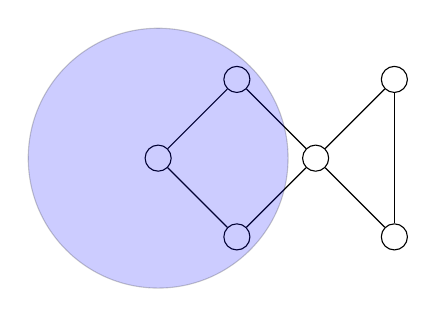
\begin{tikzpicture}
        \node[draw, circle] (n1) at (0,0) {};
        \node[draw, circle] (n2) at (1,1) {};
        \node[draw, circle] (n4) at (1,-1) {};
        \node[draw, circle] (n3) at (2,0) {};
        \node[draw, circle] (n5) at (3,-1) {};
        \node[draw, circle] (n6) at (3,1) {};

        % \onslide<2->{
            \draw[-] (n1)--(n2);
            \draw[-] (n2)--(n3)--(n4);
            \draw[-] (n4)--(n1);
            \draw[-] (n3)--(n6);
            \draw[-] (n6)--(n5);
            \draw[-] (n5)--(n3);
        % }
            \draw[fill=blue, opacity=0.2] (0,0) circle (1.65);
        
        % \onslide<3->{
        %     \draw[red, -] (n1)--(n2);
        %     \draw[red, -] (n2)--(n3)--(n4);
        %     \draw[-] (n4)--(n1);
        %     \draw[-, red] (n3)--(n6);
        %     \draw[-] (n6)--(n5);
        %     \draw[-, red] (n5)--(n3);
        % }

        \draw[transparent, rounded corners, rotate around={45:(0,-0.5)}, dotted] (0,-0.5) rectangle (2.2,0.3);
        \draw[transparent, rounded corners, rotate around={-45:(0,0.5)}, dotted] (0,0.5) rectangle (2.2,-0.3);
    \end{tikzpicture}

   Graph rewriting:
    \begin{itemize}
        \item computational units $\rightarrow$ nodes
        \item communication channels  $\rightarrow$ edges
        \item system states  $\rightarrow$ graphs
        \item algorithm behaviors $\rightarrow$ graph transformation rules
    \end{itemize}
\end{frame}

\begin{frame}{Graph Transformation}
 Graph representing a configuration of a distributed system:

    \begin{overlayarea}{\textwidth}{\textheight}
        \begin{center}
        \begin{onlyenv}<1>
            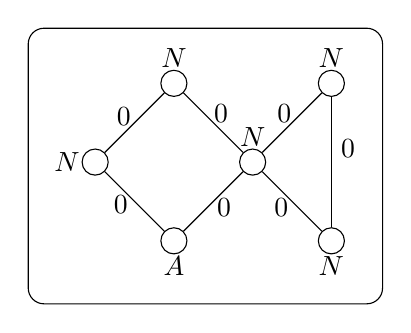
\begin{tikzpicture}
            \graphbox{}{0mm}{0mm}{45mm}{35mm}{-14mm}{-17mm}{
            \node[draw, circle, label={[label distance=-1mm]left:{$N$}}] (n1) at (0,0) {};
            \node[draw, circle, label={[label distance=-1mm]above:{$N$}}] (n2) at (1,1) {};
            \node[draw, circle, label={[label distance=-1mm]above:{$N$}}] (n3) at (2,0) {};
            \node[draw, circle, label={[label distance=-1mm]below:{$A$}}] (n4) at (1,-1) {};
            \node[draw, circle, label={[label distance=-1mm]below:{$N$}}] (n5) at (3,-1) {};
            \node[draw, circle, label={[label distance=-1mm]above:{$N$}}] (n6) at (3,1) {};
            \draw[-] (n1)-- node[pos=0.6, left] {$0$} (n2);
            \draw[-] (n2)-- node[pos=0.35,right] {$0$} (n3);
            \draw[-] (n3)-- node[pos=0.6,right] {$0$}(n4);
            \draw[-] (n4)-- node[pos=0.45,left] {$0$}(n1);
            \draw[-] (n3)-- node[pos=0.65,left] {$0$}(n6);
            \draw[-] (n6)-- node[pos=0.4,right] {$0$}(n5);
            \draw[-] (n5)-- node[pos=0.4,left] {$0$}(n3);
            }
        \end{tikzpicture}
        % } 
        \end{onlyenv}
            \begin{onlyenv}<2>
            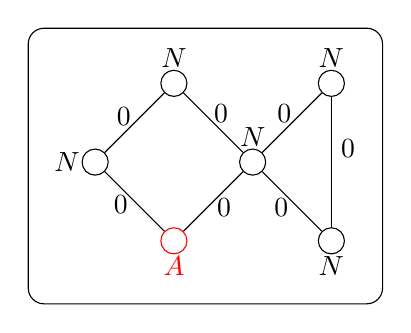
\begin{tikzpicture}
            \graphbox{}{0mm}{0mm}{45mm}{35mm}{-14mm}{-17mm}{
            \node[draw, circle, label={[label distance=-1mm]left:{$N$}}] (n1) at (0,0) {};
            \node[draw, circle, label={[label distance=-1mm]above:{$N$}}] (n2) at (1,1) {};
            \node[draw, circle, label={[label distance=-1mm]above:{$N$}}] (n3) at (2,0) {};
            \node[red, draw, circle, label={[label distance=-1mm]below:{\textcolor{red}{$A$}}}] (n4) at (1,-1) {};
            \node[draw, circle, label={[label distance=-1mm]below:{$N$}}] (n5) at (3,-1) {};
            \node[draw, circle, label={[label distance=-1mm]above:{$N$}}] (n6) at (3,1) {};
            \draw[-] (n1)-- node[pos=0.6, left] {$0$} (n2);
            \draw[-] (n2)-- node[pos=0.35,right] {$0$} (n3);
            \draw[-] (n3)-- node[pos=0.6,right] {$0$}(n4);
            \draw[-] (n4)-- node[pos=0.45,left] {$0$}(n1);
            \draw[-] (n3)-- node[pos=0.65,left] {$0$}(n6);
            \draw[-] (n6)-- node[pos=0.4,right] {$0$}(n5);
            \draw[-] (n5)-- node[pos=0.4,left] {$0$}(n3);
            }
        \end{tikzpicture}
        % } 
        \end{onlyenv}
            %2
        \begin{onlyenv}<3>
    % \resizebox{0.28\textwidth}{!}{
      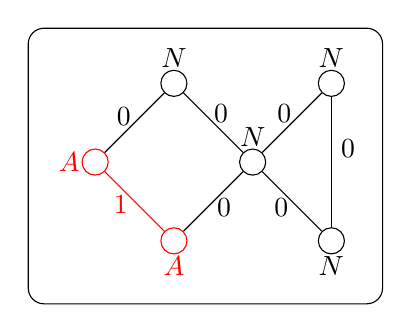
\begin{tikzpicture}
        \graphbox{}{0mm}{0mm}{45mm}{35mm}{-14mm}{-17mm}{
        \node[red,draw, circle, label={[label distance=-1mm]left:{\textcolor{red}{$A$}}}] (n1) at (0,0) {};
        \node[draw, circle, label={[label distance=-1mm]above:{$N$}}] (n2) at (1,1) {};
        \node[draw, circle, label={[label distance=-1mm]above:{$N$}}] (n3) at (2,0) {};
        \node[red, draw, circle, label={[label distance=-1mm]below:{\textcolor{red}{$A$}}}] (n4) at (1,-1) {};
        \node[draw, circle, label={[label distance=-1mm]below:{$N$}}] (n5) at (3,-1) {};
        \node[draw, circle, label={[label distance=-1mm]above:{$N$}}] (n6) at (3,1) {};
        \draw[-] (n1)-- node[pos=0.6, left] {$0$} (n2);
        \draw[-] (n2)-- node[pos=0.35,right] {$0$} (n3);
        \draw[-] (n3)-- node[pos=0.6,right] {$0$}(n4);
        \draw[-,red] (n4)-- node[pos=0.45,left] {\textcolor{red}{$1$}}(n1);
        \draw[-] (n3)-- node[pos=0.65,left] {$0$}(n6);
        \draw[-] (n6)-- node[pos=0.4,right] {$0$}(n5);
        \draw[-] (n5)-- node[pos=0.4,left] {$0$}(n3);
        }
        \end{tikzpicture}
    % }
        \end{onlyenv}
    %3
    \begin{onlyenv}<4>
    % \resizebox{0.28\textwidth}{!}{
       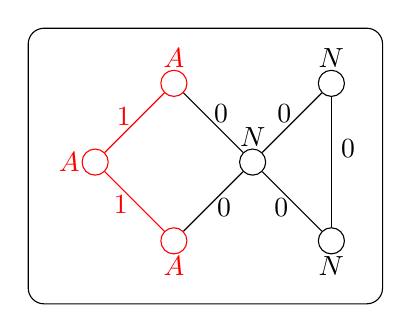
\begin{tikzpicture}  
        \graphbox{}{0mm}{0mm}{45mm}{35mm}{-14mm}{-17mm}{
        \node[red,draw, circle, label={[label distance=-1mm]left:{\textcolor{red}{$A$}}}] (n1) at (0,0) {}; 
        \node[red,draw, circle, label={[label distance=-1mm]above:{\textcolor{red}{$A$}}}] (n2) at (1,1) {};
        \node[draw, circle, label={[label distance=-1mm]above:{$N$}}] (n3) at (2,0) {};
        \node[red, draw, circle, label={[label distance=-1mm]below:{\textcolor{red}{$A$}}}] (n4) at (1,-1) {};
        \node[draw, circle, label={[label distance=-1mm]below:{$N$}}] (n5) at (3,-1) {}; 
        \node[draw, circle, label={[label distance=-1mm]above:{$N$}}] (n6) at (3,1) {};
        \draw[red,-] (n1)-- node[pos=0.6, left] {\textcolor{red}{$1$}} (n2);
        \draw[-] (n2)-- node[pos=0.35,right] {$0$} (n3);
        \draw[-] (n3)-- node[pos=0.6,right] {$0$}(n4);
        \draw[-,red] (n4)-- node[pos=0.45,left] {\textcolor{red}{$1$}}(n1);
        \draw[-] (n3)-- node[pos=0.65,left] {$0$}(n6);
        \draw[-] (n6)-- node[pos=0.4,right] {$0$}(n5);
        \draw[-] (n5)-- node[pos=0.4,left] {$0$}(n3);
        }
    \end{tikzpicture}
    % }
    \end{onlyenv}

    %4
    \begin{onlyenv}<5>
    % \resizebox{0.28\textwidth}{!}{
     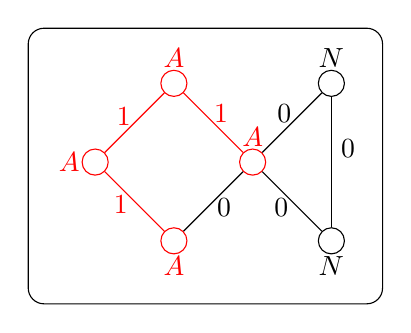
\begin{tikzpicture}  
        \graphbox{}{0mm}{0mm}{45mm}{35mm}{-14mm}{-17mm}{
        \node[red,draw, circle, label={[label distance=-1mm]left:{\textcolor{red}{$A$}}}] (n1) at (0,0) {}; 
        \node[red,draw, circle, label={[label distance=-1mm]above:{\textcolor{red}{$A$}}}] (n2) at (1,1) {};
        \node[red,draw, circle, label={[label distance=-1mm]above:{\textcolor{red}{$A$}}}] (n3) at (2,0) {};
        \node[red, draw, circle, label={[label distance=-1mm]below:{\textcolor{red}{$A$}}}] (n4) at (1,-1) {};
        \node[draw, circle, label={[label distance=-1mm]below:{$N$}}] (n5) at (3,-1) {}; 
        \node[draw, circle, label={[label distance=-1mm]above:{$N$}}] (n6) at (3,1) {};
        \draw[red,-] (n1)-- node[pos=0.6, left] {\textcolor{red}{$1$}} (n2);
        \draw[red,-] (n2)-- node[pos=0.35,right] {\textcolor{red}{$1$}} (n3);
        \draw[-] (n3)-- node[pos=0.6,right] {$0$}(n4);
        \draw[-,red] (n4)-- node[pos=0.45,left] {\textcolor{red}{$1$}}(n1);
        \draw[-] (n3)-- node[pos=0.65,left] {$0$}(n6);
        \draw[-] (n6)-- node[pos=0.4,right] {$0$}(n5);
        \draw[-] (n5)-- node[pos=0.4,left] {$0$}(n3);
        }
    \end{tikzpicture}
    % }
    \end{onlyenv}

    %5
    \begin{onlyenv}<6>
    % \resizebox{0.28\textwidth}{!}{
    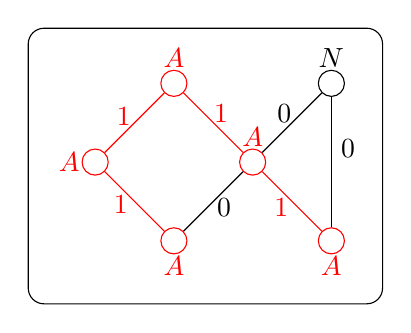
\begin{tikzpicture}  
        \graphbox{}{0mm}{0mm}{45mm}{35mm}{-14mm}{-17mm}{
        \node[red,draw, circle, label={[label distance=-1mm]left:{\textcolor{red}{$A$}}}] (n1) at (0,0) {}; 
        \node[red,draw, circle, label={[label distance=-1mm]above:{\textcolor{red}{$A$}}}] (n2) at (1,1) {};
        \node[red,draw, circle, label={[label distance=-1mm]above:{\textcolor{red}{$A$}}}] (n3) at (2,0) {};
        \node[red, draw, circle, label={[label distance=-1mm]below:{\textcolor{red}{$A$}}}] (n4) at (1,-1) {};
        \node[red,draw, circle, label={[label distance=-1mm]below:{\textcolor{red}{$A$}}}] (n5) at (3,-1) {}; 
        \node[draw, circle, label={[label distance=-1mm]above:{$N$}}] (n6) at (3,1) {};
        \draw[red,-] (n1)-- node[pos=0.6, left] {\textcolor{red}{$1$}} (n2);
        \draw[red,-] (n2)-- node[pos=0.35,right] {\textcolor{red}{$1$}} (n3);
        \draw[-] (n3)-- node[pos=0.6,right] {$0$}(n4);
        \draw[-,red] (n4)-- node[pos=0.45,left] {\textcolor{red}{$1$}}(n1);
        \draw[-] (n3)-- node[pos=0.65,left] {$0$}(n6);
        \draw[-] (n6)-- node[pos=0.4,right] {$0$}(n5);
        \draw[red,-] (n5)-- node[pos=0.4,left] {\textcolor{red}{$1$}}(n3);
        }
    \end{tikzpicture}
    % }
    \end{onlyenv}
    %6
    \begin{onlyenv}<7->
    % \resizebox{0.28\textwidth}{!}{
    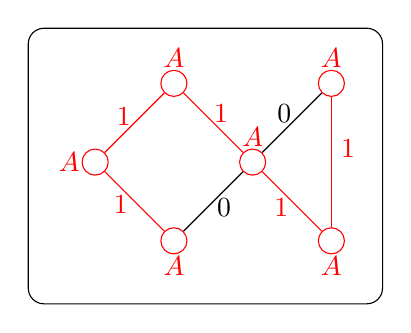
\begin{tikzpicture}  
        \graphbox{}{0mm}{0mm}{45mm}{35mm}{-14mm}{-17mm}{
        \node[red,draw, circle, label={[label distance=-1mm]left:{\textcolor{red}{$A$}}}] (n1) at (0,0) {}; 
        \node[red,draw, circle, label={[label distance=-1mm]above:{\textcolor{red}{$A$}}}] (n2) at (1,1) {};
        \node[red,draw, circle, label={[label distance=-1mm]above:{\textcolor{red}{$A$}}}] (n3) at (2,0) {};
        \node[red, draw, circle, label={[label distance=-1mm]below:{\textcolor{red}{$A$}}}] (n4) at (1,-1) {};
        \node[red,draw, circle, label={[label distance=-1mm]below:{\textcolor{red}{$A$}}}] (n5) at (3,-1) {}; 
        \node[red,draw, circle, label={[label distance=-1mm]above:{\textcolor{red}{$A$}}}] (n6) at (3,1) {};
        \draw[red,-] (n1)-- node[pos=0.6, left] {\textcolor{red}{$1$}} (n2);
        \draw[red,-] (n2)-- node[pos=0.35,right] {\textcolor{red}{$1$}} (n3);
        \draw[-] (n3)-- node[pos=0.6,right] {$0$}(n4);
        \draw[-,red] (n4)-- node[pos=0.45,left] {\textcolor{red}{$1$}}(n1);
        \draw[-] (n3)-- node[pos=0.65,left] {$0$}(n6);
        \draw[red,-] (n6)-- node[pos=0.4,right] {\textcolor{red}{$1$}}(n5);
        \draw[red,-] (n5)-- node[pos=0.4,left] {\textcolor{red}{$1$}}(n3);
        }
    \end{tikzpicture}
    \end{onlyenv}
     \end{center}

    Graph transformation rule:
        \begin{center}
        \resizebox{0.7\textwidth}{!}{
            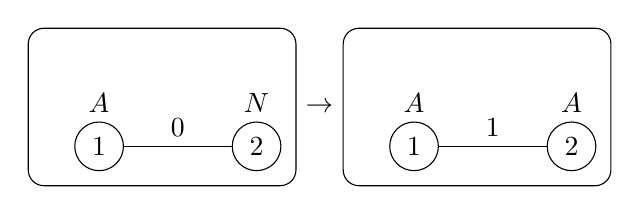
\begin{tikzpicture}
                        \graphbox{\(\)}{0mm}{0mm}{34mm}{20mm}{-8mm}{-15mm}{
                            \node[draw, circle] (x) at (0,0) {$1$};
                            \node () at (0,0.55) {$A$};  
                            \node[draw, circle] (y) at (2,0) {$2$};
                            \node () at (2,0.55) {$N$};
                            \draw[-] (x) -- node[midway,above] {$0$} (y) ;
                            %             \draw[->] (x) edge [loop above] node {$A$} (x);
                            % \draw[->] (y) edge [loop above] node {$N$} (y);
                        }
                        \graphbox{\(\)}{40mm}{0mm}{34mm}{20mm}{-8mm}{-15mm}{
                            \node[draw, circle]  (x) at (0,0) {$1$};  
                            \node () at (0,0.55) {$A$};  
                            \node[draw, circle]  (y) at (2,0) {$2$};
                            \node () at (2,0.55) {$A$};
                            \draw[-] (x) -- node[midway,above] {$1$} (y) ;
                            % \draw[->] (x) edge [loop above] node {$A$} (x);
                            % \draw[->] (y) edge [loop above] node {$A$} (y);
                        }  
                        \node () at (37mm,-10mm) {\( \mathop{\rightarrow} \)}; % K -> L
            \end{tikzpicture}
        } 
        \end{center}
        \begin{onlyenv}<8>
            Question: does the transformation process terminate from any initial configuration?
        \end{onlyenv} 
    \end{overlayarea}
    
    \note{The graph models a distributed network of six computational units.
Each node represents a computational unit; a node's state is indicated by the label of its self-loop; each edge represents a communication channel. node $1$ labeled by $A$ represents an active computational unit, the other nodes labeled by $N$ represent neutral computational units, and edges labeled by $0$ represent communication channels in state $0$.}

\note{The algorithm operates as follows: when an active unit detects a neutral neighbor via a channel in state $0$, it activates the neighbor and updates the channel to state $1$.
 This behavior is captured by the graph transformation rule in Figure~\ref{fig:intro:graph_transformation_rule_0}.}
\end{frame}

\begin{frame}{Termination of graph transformation systems}
  \begin{itemize}
    \item $\mathcal{R}$ : a set of rules
    \item No graph $G_0$ can be transformed forever
         $$G_0 \Rightarrow G_1 \Rightarrow \cdots$$
         when using the non-deterministic strategy 
          \begin{center}
              \textcolor{blue}{\enquote{apply rules as long as possible}}
          \end{center}
    \item Aligns with the standard notion of program termination: 
         \begin{center}
            \textcolor{blue}{\enquote{every execution (on any input) eventually halts.}}
          \end{center}
    \item Undecidable in general 
  \end{itemize}
\end{frame}


\begin{frame}{One-rule examples of non-termination and termination}
 
        \noindent Rule $\alpha$ :\resizebox{0.5\textwidth}{!}{
                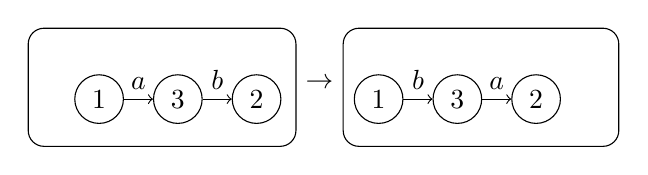
\begin{tikzpicture}[baseline=-10mm]
                    \graphbox{}{0mm}{-3mm}{34mm}{15mm}{2mm}{2mm}{
                        \coordinate (o) at (0mm,-11mm); 
                        \node[draw,circle] (l1) at ($(o)+(-10mm,0mm)$) {1};
                        \node[draw,circle] (l2) at ($(l1)+(2,0)$) {2};
                        \node[draw,circle] (l3) at ($(l1)+(1,0)$) {3};
                        \draw[->] (l1) -- (l3) node[midway,above] {$a$};
                        \draw[->] (l3) -- (l2) node[midway,above] {$b$};
                    } 
            
                    % \graphbox{\( K \)}{40mm}{-3mm}{34mm}{15mm}{2mm}{2mm}{
                    %     \coordinate (o) at (0mm,-11mm); 
                    %     \node[draw,circle] (l1) at ($(o)+(-10mm,0mm)$) {1};
                    %     \node[draw,circle] (l2) at ($(l1)+(2,0)$) {2};
                    % }  
            
                    \graphbox{}{40mm}{-3mm}{35mm}{15mm}{2mm}{2mm}{
                        \coordinate (o) at (-5mm,-11mm); 
                        \node[draw,circle] (l1) at ($(o)+(-10mm,0mm)$) {1};
                        % \node[draw,circle] (l2) at ($(l1)+(3,0)$) {2};
                        \node[draw,circle] (l3) at ($(l1)+(1,0)$) {3};
                        \node[draw,circle] (l4) at ($(l1)+(2,0)$) {2};
                        \draw[->] (l1) -- (l3) node[midway,above] {$b$};
                        \draw[->] (l3) -- (l4) node[midway,above] {$a$};
                        % \draw[->] (l4) -- (l2) node[midway,above] {$a$};
                    }    
                    % \node () at (37mm,-10mm) {\( \leftarrow \)}; % K -> L
                    \node () at (37mm,-10mm) {\( \rightarrow \)}; % K -> R
                \end{tikzpicture}
                }
      
 
                \vspace{4mm}
        
            \noindent Looping:\resizebox{0.85\textwidth}{!}{
              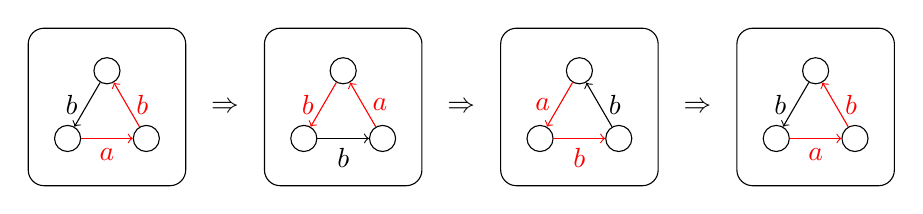
\begin{tikzpicture}[baseline=-10mm]
              \graphbox{\( \)}{0mm}{0mm}{20mm}{20mm}{-5mm}{-14mm}{
                  \node[draw,circle] (x) at (0,0) {};
                  \node[draw,circle] (y) at (1,0) {};
                  \node[draw,circle] (z) at (0.5,0.86) {};
                  \draw[->,red] (x) -- node[midway,below] {$a$} (y) ;
                  \draw[->,red] (y) -- node[midway,right] {$b$} (z) ;
                  \draw[->] (z) -- node[midway,left] {$b$} (x) ;
              } 
              \node () at (25mm,-10mm) {\( \Rightarrow  \)};
              \graphbox{\( \)}{30mm}{0mm}{20mm}{20mm}{-5mm}{-14mm}{
                  \node[draw,circle] (x) at (0,0) {};  
                  \node[draw,circle] (y) at (1,0) {};
                  \node[draw,circle] (z) at (0.5,0.86) {};
                  \draw[->] (x) -- node[midway,below] {$b$} (y) ;
                  \draw[->,red] (y) -- node[midway,right] {$a$} (z) ;
                  \draw[->,red] (z) -- node[midway,left] {$b$} (x) ;
              } 
              \node () at (55mm,-10mm) {\( \Rightarrow  \)};
              \graphbox{\( \)}{60mm}{0mm}{20mm}{20mm}{-5mm}{-14mm}{
                  \node[draw,circle] (x) at (0,0) {};  
                  \node[draw,circle] (y) at (1,0) {};
                  \node[draw,circle] (z) at (0.5,0.86) {};
                  \draw[->,red] (x) -- node[midway,below] {$b$} (y) ;
                  \draw[->] (y) -- node[midway,right] {$b$} (z) ;
                  \draw[->,red] (z) -- node[midway,left] {$a$} (x) ;
              }
              \node () at (85mm,-10mm) {\( \Rightarrow  \)};
              \graphbox{\( \)}{90mm}{0mm}{20mm}{20mm}{-5mm}{-14mm}{
                  \node[draw,circle] (x) at (0,0) {};   
                  \node[draw,circle] (y) at (1,0) {};
                  \node[draw,circle] (z) at (0.5,0.86) {};
                  \draw[->,red] (x) -- node[midway,below] {$a$} (y) ;
                  \draw[->,red] (y) -- node[midway,right] {$b$} (z) ;
                  \draw[->] (z) -- node[midway,left] {$b$} (x) ;
              }
          \end{tikzpicture}
          }
   

     
                \vspace{4mm}
   
        \noindent Rule $\beta$:\resizebox{0.5\textwidth}{!}{ 
       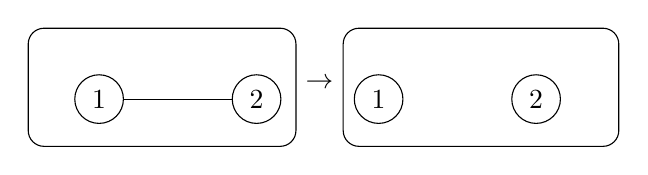
\begin{tikzpicture}[baseline=-10mm]
                    \graphbox{}{0mm}{-3mm}{34mm}{15mm}{2mm}{2mm}{
                        \coordinate (o) at (0mm,-11mm); 
                        \node[draw,circle] (l1) at ($(o)+(-10mm,0mm)$) {1};
                        \node[draw,circle] (l2) at ($(l1)+(2,0)$) {2};
                        % \node[draw,circle] (l3) at ($(l1)+(1,0)$) {3};
                        \draw[-] (l1) -- (l2) node[midway,above] {};
                    } 
                    % \graphbox{\( K \)}{40mm}{-3mm}{34mm}{15mm}{2mm}{2mm}{
                    %     \coordinate (o) at (0mm,-11mm); 
                    %     \node[draw,circle] (l1) at ($(o)+(-10mm,0mm)$) {1};
                    %     \node[draw,circle] (l2) at ($(l1)+(2,0)$) {2};
                    % }  
                    \graphbox{}{40mm}{-3mm}{35mm}{15mm}{2mm}{2mm}{
                        \coordinate (o) at (-5mm,-11mm); 
                        \node[draw,circle] (l1) at ($(o)+(-10mm,0mm)$) {1};
                        % \node[draw,circle] (l2) at ($(l1)+(3,0)$) {2};
                         % \node[draw,circle] (l3) at ($(l1)+(1,0)$) {4};
                        \node[draw,circle] (l4) at ($(l1)+(2,0)$) {2};
                        % \draw[->] (l1) -- (l4) node[midway,above] {};
                        % \draw[->] (l4) -- (l2) node[midway,above] {$a$};
                    }    
                    \node () at (37mm,-10mm) {\( \rightarrow \)}; % K -> L
                    % \node () at (77mm,-10mm) {\( \rightarrow \)}; % K -> R
                \end{tikzpicture}
                }

                \vspace{4mm}
\noindent Terminating by the number of edges if we consider finite graphs only.
\end{frame}


\begin{frame}{Motivating Rule}
     \begin{center}
        \resizebox{\textwidth}{!}{ 
            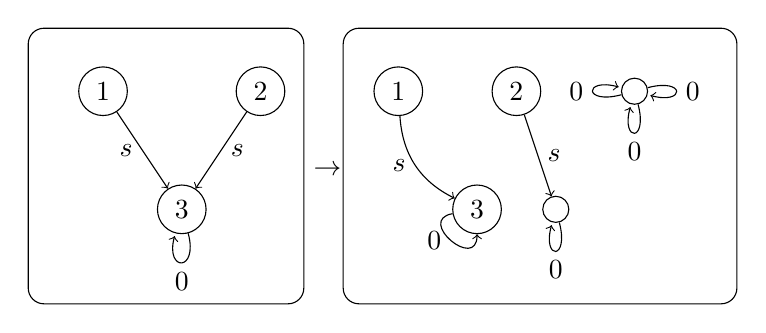
\begin{tikzpicture}
                \graphbox{}{0mm}{0mm}{35mm}{35mm}{2mm}{-5mm}{
                    \coordinate (delta) at (0,-18mm);
                    \node[draw,circle] (l1) at ($(delta)+(-1,1.5)$) {1};
                    \node[draw,circle] (l2) at ($(delta)+(1,1.5)$) {2};
                    \node[draw,circle] (l3) at ($(delta)+(0,0)$) {3};
                    \draw[->] (l1) -- (l3) node[midway,left] {$s$};
                    \draw[->] (l2) -- (l3) node[midway,right] {$s$};
                    \draw[->] (l3) edge [loop below] node {0} (l3);
                }
                    % \graphbox{$K$}{40mm}{0mm}{35mm}{35mm}{2mm}{-5mm}{
                    %     \coordinate (delta) at (0,-18mm);
                    %     \coordinate (interfaceorigin) at ($(delta) +(5,0)$);
                    %     \node[draw,circle] (r1) at ($(delta) +(-1,1.5)$) {1};
                    %     \node[draw,circle] (r2) at ($(delta) +(0.5,1.5)$) {2};
                    %     \node[draw,circle] (r3) at ($(delta)+(0,0)$) {3};
                    %     % \draw[->] (r1) -- (r3) node[midway,left] {$s$};
                    %     % \draw[->] (r3) edge [loop below] node {0} (r3);
                    % } 
                    \node () at (38mm,-18mm) {$\rightarrow$};
                    % \node () at (77mm,-18mm) {$\rightarrow$};
                \graphbox{}{40mm}{0mm}{50mm}{35mm}{2mm}{-5mm}{
                    \coordinate (delta) at (-10mm,-18mm);
                    \node[draw,circle] (r1) at ($(delta)+(-1,1.5)$) {1};
                    \node[draw,circle] (r2) at ($(delta)+(0.5,1.5)$) {2};
                    \node[draw,circle] (r3) at ($(delta)+(0,0)$) {3};
                    \node[draw,circle] (r4) at ($(delta)+(1,0)$) {};
                    \draw[->] (r1) edge[bend right] node[midway,left] {$s$} (r3) ;
                    \draw[->] (r2) -- (r4) node[midway,right] {$s$};
                    \draw[->] (r4) edge [loop below] node {0} (r4);
                    
                    \draw[->] (r3) edge [out=190,in=270,looseness=3] node[midway,left] {0} (r3);
                    \node[draw,circle] (r5) at ($(r2)+(1.5,0)$) {};
                    \draw[->] (r5) edge [loop below] node {0} (r5);
                    \draw[->] (r5) edge [loop right] node {0} (r5);
                    \draw[->] (r5) edge [loop left] node {0} (r5);
                }
            \end{tikzpicture}
            }
    \end{center}

    Question: does this rule terminate?
\end{frame}


\section{Preliminaries}
\begin{frame}{Structure of the presentation}
    \tableofcontents[hideothersubsections]
\end{frame}
% \subsection{Graphs and graph morphisms}
\begin{frame}{Graphs : finite, directed, edge-labeled multigraphs}
\begin{adjustwidth}{-0.5cm}{0cm}
        \begin{center} 
          \resizebox{0.5\textwidth}{!}{
          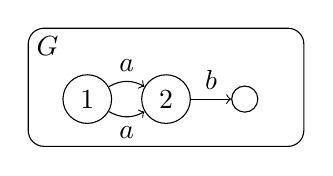
\begin{tikzpicture}
              \graphbox{\(G\)}{0mm}{-20mm}{35mm}{15mm}{2mm}{-5mm}{ 
                  \coordinate (o) at (-2mm,-4mm); 
                  \node[draw,circle] (l1) at ($(o)+(-10mm,0mm)$) {1};
                  \node[draw,circle] (l3) at ($(l1)+(1,0)$) {2};
                  \node[draw,circle] (l4) at ($(l1)+(2,0)$) {};
                  \draw[->] (l1) edge[bend right]  node[midway,below] {$a$} (l3);
                  \draw[->] (l1) edge[bend left] node[midway,above] {$a$}  (l3);
                  \draw[->] (l3) -- (l4) node[midway,above] {$b$};
                  % \draw[->] (l4) -- (l2) node[midway,above] {$a$};
              }   
          \end{tikzpicture} 
      }
      \end{center}
      Remarks:
      \begin{itemize}
            \item Edges with the same source, target and label are permitted.
            % \item Enclosed in a box
            \item Graph name (\(G\)) shown at the top left of the drawing.
            \item Numbers inside nodes are identifiers (omitted when not relevant).
      \end{itemize}
\end{adjustwidth}
\end{frame} 

\begin{frame}{Graph morphisms: structure-preserving functions}
\begin{adjustwidth}{-0.5cm}{0cm}
             \begin{center}
          \resizebox{0.8\textwidth}{!}{
          \begin{tikzpicture}
            \graphbox{\( G \)}{0mm}{-20mm}{45mm}{25mm}{2mm}{-10mm}{
                \coordinate (o) at (-5mm,-8mm); 
                \node[draw,circle] (l1) at ($(o)+(-10mm,0mm)$) {1};
                \node[draw,circle] (l2) at ($(l1)+(3,0)$) {2};
                \node[draw,circle] (l3) at ($(l1)+(1,0)$) {3};
                \node[draw,circle] (l4) at ($(l1)+(2,0)$) {4};
                \draw[->] (l1) -- (l3) node[midway,above] {$a$};
                \draw[->] (l3) -- (l4) node[midway,above] {$b$};
                \draw[->] (l4) -- (l2) node[midway,above] {$a$};
            }  
            \graphbox{\( H \)}{52mm}{-20mm}{50mm}{25mm}{2mm}{-10mm}{
                \coordinate (o) at (-5mm,-8mm); 
                \node[draw,circle] (l1) at ($(o)+(-1,0mm)$) {1};
                \node[draw,circle] (l2) at ($(l1)+(3,0)$) {2};
                \node[draw,circle] (l3) at ($(l1)+(1.5,0)$) {3\ 4};
                \draw[->] (l1) edge node[midway,above] {$a$} (l3);
                \draw[->] (l3) edge [loop above] node[midway,above] {$b$} (l3) ;
                \draw[->] (l3) -- (l2) node[midway,above] {$a$};
            }      
            \node () at (48mm,-30mm) {$\overset{h}{\rightarrow}$};
        \end{tikzpicture}
          }
         \end{center}
        Remarks:
        \begin{itemize}
            \item Nodes of H are labeled with the sets of identifiers of nodes of $G$ that map to them.
            \item $\overset{h}{\rightarrow}$ indicates $h: G \rightarrow H$.
        \end{itemize}
\end{adjustwidth}
\end{frame}

% \subsection{Pushouts}
\begin{frame}{Commutative Diagram}
    \begin{beamercolorbox}[wd=\textwidth,sep=1.2ex]{block body}
        \begin{center}
            \resizebox{0.3\textwidth}{!}{
                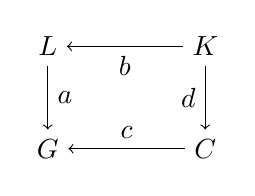
\begin{tikzpicture}
                    \node (I) at (0,-0.7) {$K$};
                    \node (L) at (-2,-0.7) {$L$};
                    \node (G) at (-2,-2) {$G$};
                    \node (C) at (0,-2) {$C$};
                    \draw [->] (I) to  node [midway,below] {$b$} (L);
                    \draw [->] (L) to node [midway,right] {$a$} (G);
                    \draw [->] (I) to node [midway,left] {$d$} (C);
                    \draw [->] (C) to node [midway,above] {$c$} (G);
                \end{tikzpicture}
            } 
        \end{center}
        Commutative if \( a \circ b = c \circ d \).
    \end{beamercolorbox}
        
        \begin{center}
                \begin{tikzpicture}
                    \graphbox{}{0mm}{0mm}{34mm}{15mm}{2mm}{0mm}{
                        \coordinate (o) at (0mm,-8mm); 
                        \node[draw,circle] (l1) at ($(o)+(-10mm,0mm)$) {1};
                        \node[draw,circle] (l2) at ($(l1)+(2,0)$) {2};
                        \node[draw,circle] (l3) at ($(l1)+(1,0)$) {};
                        \draw[->] (l1) -- (l3) node[midway,above] {};
                        \draw[->] (l3) -- (l2) node[midway,above] {};
                    } 
                    \graphbox{}{40mm}{0mm}{34mm}{15mm}{2mm}{0mm}{
                        \coordinate (o) at (0mm,-8mm); 
                        \node[draw,circle] (l1) at ($(o)+(-10mm,0mm)$) {1};
                        \node[draw,circle] (l2) at ($(l1)+(2,0)$) {2};
                    }  
                
                    \graphbox{ }{0mm}{-22mm}{34mm}{25mm}{2mm}{-5mm}{
                        \coordinate (o) at (0mm,-3mm); 
                        \node[draw,circle] (l1) at ($(o)+(-10mm,0mm)$) {1};
                        \node[draw,circle] (l2) at ($(l1)+(2,0)$) {2};
                        \node[draw,circle ] (l3) at ($(l1)+(1,0)$) {};
                        \node[draw,circle] (l4) at ($(l2)+(0,-1)$) {};
                        \draw[->] (l1) -- (l3) node[midway,above] {};
                        \draw[->] (l3) -- (l2) node[midway,above] {};
                        \draw[->] (l2) -- (l4) node[midway,right] {};
                    }    
                    \graphbox{ }{40mm}{-22mm}{34mm}{25mm}{2mm}{-5mm}{
                        \coordinate (o) at (0mm,-3mm); 
                        \node[draw,circle] (l1) at ($(o)+(-10mm,0mm)$) {1};
                        \node[draw,circle] (l2) at ($(l1)+(2,0)$) {2};
                        \node[draw,circle] (l4) at ($(l2)+(0,-1)$) {};
                        \draw[->] (l2) -- (l4) node[midway,right] {};
                    }    
                    \node () at (37mm,-8mm) {\( \underset{b}{\leftarrow} \)};  
                    \node () at (17mm,-18mm) {\( \downarrow\ a \)};
                    \node () at (37mm,-33mm) {\( \overset{c}{\leftarrow} \)};
                    \node () at (52mm,-18mm) {\( d\ \downarrow \)};
            \end{tikzpicture}
        \end{center}
\end{frame}

\begin{frame}{Pushouts: gluing graphs along a common part}
    \begin{definition}
    The \textbf{pushout} of \((\alpha,\beta) \)
    is \begin{onlyenv}<2->
        \( \textcolor{red}{(\beta',\alpha')}\) such that
    \end{onlyenv}
    \begin{itemize}
        % \item<2->{commutation:} \textcolor{red}{\( \beta' \mathop{\circ} \alpha  \mathop{=} \alpha'\mathop{\circ} \beta\)},
        \item<2-> \text{ABDC} is commutative,
        % \item<3->{universality:}  \textcolor{PineGreen}{\( \forall \alpha \mathop{\star} \gamma' \mathop{=} \beta \mathop{\star} \gamma \Longrightarrow \exists~!~\delta. \gamma' \mathop{=} \beta' \mathop{\star} \delta  \gamma \mathop{=} \alpha' \mathop{\star} \delta \)}.
        \item<3->{universality:}  \textcolor{PineGreen}{\( \forall (\gamma,\gamma').~\text{ABEC is commutative} \Longrightarrow \exists~!~\delta.~ \text{BDE \& CDE are commutative} \)}.
    \end{itemize} 
\end{definition} 
\hspace{-0.075\textwidth}% <-- exact horizontal gap between the two minipages
\begin{minipage}[t]{0.2\textwidth}
  \begin{overlayarea}{0.2\textwidth}{0.6\textheight}
    \begin{tikzpicture}[scale=0.8]
            \node (i) at (0,0) {A};
            \node (r) at (-1.5,-1) {B};
            \node (c) at (1.5,-1) {C};
            % \node () at (1,-1) {\( \Delta \)};
            \begin{onlyenv}<1->
                \draw[->]  (i) -- (r) node [pos=0.4,left] {$ \alpha $};
                \draw[->] (i) -- (c) node[pos=0.4, right] {$ \beta $};
            \end{onlyenv}
            \begin{onlyenv}<2->
                \node (h) at (0,-2) {\textcolor{red}{D}};
                    \draw[red,->] (c) -- (h) node [pos=0.8,right=1mm] {$ \alpha' $};
                \draw[red,->] (r) -- (h) node[pos=0.9, left=2mm] {$ \beta' $};
                \node () at (0,-1) {\textcolor{red}{PO}};
            \end{onlyenv}
            \begin{onlyenv}<3->
                \color{PineGreen}
                \node (d') at (0,-4) {E};
                \draw[->] (c) edge[bend left] node [midway,right]{$ \gamma $} (d') ;
                \draw[->] (r) edge[bend right] node [midway,left]{$ \gamma' $} (d') ;
                \draw[->,dashed] (h) -- (d') node [midway,right]{$ \delta $};
                \color{black}
            \end{onlyenv}
        \end{tikzpicture}
\end{overlayarea}
\end{minipage} 
\hspace{0.25\textwidth}% <-- exact horizontal gap between the two overlayareas
% Right box: width = 0.3\textwidth
\begin{minipage}[t]{0.2\textwidth}
  \begin{overlayarea}{0.2\textwidth}{0.6\textheight}
        \begin{onlyenv}<4->
            \resizebox{8\textwidth}{!}{
        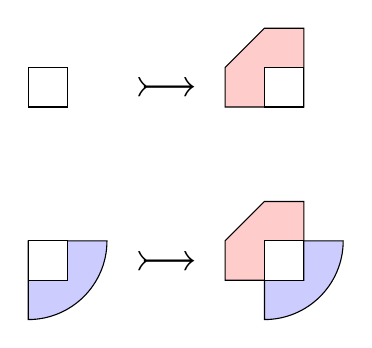
\begin{tikzpicture}  
            \coordinate (k) at (0, 0);
            \draw[fill=white] ($(k)+(0,0)$) rectangle ($(k)+(0.5,0.5)$);
            % \node () at ($(k)+(0.25,0.25)$) {\( \mathrm{K} \)};
        
            \coordinate (c) at (0, -2.2);
            \draw[fill=blue!20]
            ($(c)+(0,-0.5)$)
            -- ($(c)+(0,0.5)$) 
            -- ($(c)+(1,0.5)$) 
            arc[start angle=0, end angle=-90, radius=1]
            -- cycle;
            % \node () at ($(c)+(0.75,0.25)$) {\( \mathrm{C'} \)};
            \draw[fill=white] ($(c)+(0,0)$) rectangle ($(c)+(0.5,0.5)$);
            % \node () at ($(c)+(0.25,0.25)$) {\( \mathrm{K} \)};
    
            \coordinate (r) at (3,0);
            \draw[fill=red!20] ($(r)+(-0.5,0)$)
            -- ($(r)+(-0.5,0.5)$)
            -- ($(r)+(0,1)$)
            --  ($(r)+(0.5,1)$)
            -- ($(r)+(0.5,0)$)
            -- cycle;
            % \node () at ($(r)+(-0.23,0.25)$) {\( \mathrm{R'} \)};
            \draw[fill=white] ($(r)+(0,0)$) rectangle ($(r)+(0.5,0.5)$);
            % \node () at ($(r)+(0.25,0.25)$) {\( \mathrm{K} \)};
        
            \coordinate (h) at (3, -2.2);
            \draw[fill=blue!20]
            ($(h)+(0,-0.5)$)
            -- ($(h)+(0,0.5)$)
            -- ($(h)+(1,0.5)$) 
            arc[start angle=0, end angle=-90, radius=1]
            -- cycle;
            \draw[fill=red!20] ($(h)+(-0.5,0)$)
            -- ($(h)+(-0.5,0.5)$)
            -- ($(h)+(0,1)$)
            --  ($(h)+(0.5,1)$)
            -- ($(h)+(0.5,0)$)
            -- cycle;
        % \node () at ($(h)+(0.75,0.25)$) {\( \mathrm{C'} \)};
        \draw[fill=white] ($(h)+(0,0)$) rectangle ($(h)+(0.5,0.5)$);
        % \node () at ($(h)+(0.25,0.25)$) {\( \mathrm{K} \)};
        % \node () at ($(h)+(-0.23,0.25)$) {\( \mathrm{R'} \)};
        
            \node[ font=\huge] (kr) at ($(k)!0.5!(r)+(0.25,0.25)$)
            {\( \rightarrowtail \)}
            ;  
            \node[ font=\huge] (ch) at ($(c)!0.5!(h)+(0.25,0.25)$)
            {\( \rightarrowtail \)}
        ; 
            \node[ font=\huge] (kc) at ($(k)!0.5!(c)+(0.2,0.4)$) {\( \downarrowtail \)}; 
            \node[ font=\huge] (rh) at ($(r)!0.5!(h)+(0.1,0.4)$) {\( \downarrowtail \)}; 
        \end{tikzpicture}
            }
    \end{onlyenv}
    \end{overlayarea}
\end{minipage}
\hspace{0.3\textwidth}% small gap
\begin{minipage}[t]{0.4\textwidth}
  \begin{overlayarea}{0.4\textwidth}{0.6\textheight}
    \begin{onlyenv}<5->
        \resizebox{!}{2.2\textwidth}{
             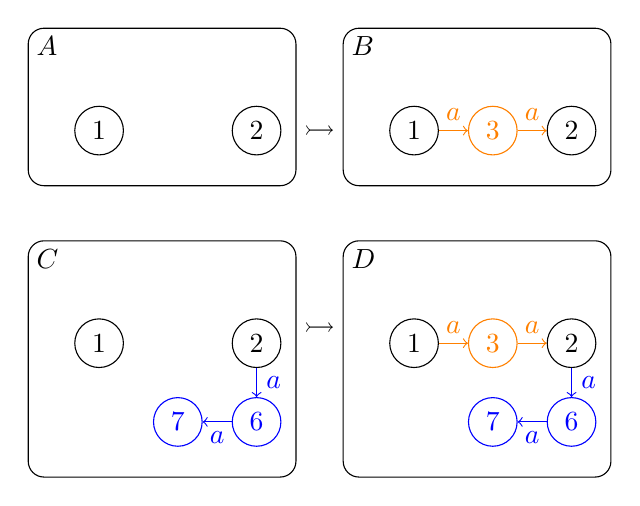
\begin{tikzpicture}
              \graphbox{\(A\)}{0mm}{5mm}{34mm}{20mm}{2mm}{-5mm}{
                 \coordinate (o) at (0mm,-8mm); 
                  \node[draw,circle] (l1) at ($(o)+(-10mm,0mm)$) {1};
                  \node[draw,circle] (l2) at ($(l1)+(2,0)$) {2};
              } 

              \graphbox{\( B \)}{40mm}{5mm}{34mm}{20mm}{2mm}{-5mm}{
                \coordinate (o) at (0mm,-8mm); 
                  \node[draw,circle] (l1) at ($(o)+(-10mm,0mm)$) {1};
                  \node[draw,circle] (l2) at ($(l1)+(2,0)$) {2};
                  \node[orange,draw,circle] (l3) at ($(l1)+(1,0)$) {3};
                  \draw[orange,->] (l1) -- (l3) node[midway,above] {$a$};
                  \draw[orange,->] (l3) -- (l2) node[midway,above] {$a$};
              }  

               
              \graphbox{\( C \)}{0mm}{-22mm}{34mm}{30mm}{2mm}{-10mm}{
                \coordinate (o) at (0mm,-3mm); 
                  \node[draw,circle] (l1) at ($(o)+(-10mm,0mm)$) {1};
                  \node[draw,circle] (l2) at ($(l1)+(2,0)$) {2};
                  \node[blue,draw,circle] (l4) at ($(l2)+(0,-1)$) {6};
                  \draw[blue,->] (l2) -- (l4) node[midway,right] {$a$};
                %   \node[blue,draw,circle] (l6) at ($(l1)+(0,-1)$) {7};
                %   \draw[blue,<-] (l1) -- (l6) node[midway,left] {$a$};
                    \node[blue,draw,circle] (l7) at ($(l4)+(-1,0)$) {7};
                  \draw[blue,->] (l4) -- (l7) node[midway,below] {$a$};
              }    

              \graphbox{\( D \)}{40mm}{-22mm}{34mm}{30mm}{2mm}{-10mm}{
                \coordinate (o) at (0mm,-3mm); 
                  \node[draw,circle] (l1) at ($(o)+(-10mm,0mm)$) {1};
                  \node[draw,circle] (l2) at ($(l1)+(2,0)$) {2};
                  \node[draw,circle,orange] (l3) at ($(l1)+(1,0)$) {3};
                  \node[blue, draw,circle] (l4) at ($(l2)+(0,-1)$) {6};
                  \draw[orange,->] (l1) -- (l3) node[midway,above] {$a$};
                  \draw[orange,->] (l3) -- (l2) node[midway,above] {$a$};
                  \draw[blue,->] (l2) -- (l4) node[midway,right] {$a$};
                %   \node[blue,draw,circle] (l6) at ($(l1)+(0,-1)$) {7};
                %   \draw[blue,<-] (l1) -- (l6) node[midway,left] {$a$};
                \node[blue,draw,circle] (l7) at ($(l4)+(-1,0)$) {7};
                  \draw[blue,->] (l4) -- (l7) node[midway,below] {$a$};
              }    

              \node () at (37mm,-8mm) {\( \rightarrowtail \)}; % K -> L
              \node () at (17mm,-18mm) {\(  \downarrowtail \)};
              \node () at (37mm,-33mm) {\( \rightarrowtail \)};
              \node () at (52mm,-18mm) {\( \downarrowtail \)};
      \end{tikzpicture}
        }
    \end{onlyenv}
  \end{overlayarea}
\end{minipage}
\end{frame}

% \begin{frame}{Pushouts}
%     \begin{overlayarea}{\textwidth}{\textheight}
%         \begin{center}
%             \begin{onlyenv}<1>
%                  \resizebox{!}{0.5\textheight}{
%                     \begin{tikzpicture}
%                             \node (i) at (0,0) {A};
%                             \node (r) at (1,1) {B};
%                             \node (c) at (1,-1) {C};
%                             \node (h) at (2,0) {D};
%                             \draw[->]  (i) -- (r) node [pos=0.6,left] {$ \alpha $};
%                             \draw[->] (c) -- (h) node [pos=0.6,left] {$ \alpha' $};
%                             \draw[->] (r) -- (h) node[pos=0.6, left] {$ \beta' $};
%                             \draw[->] (i) -- (c) node[pos=0.7, left] {$ \beta $};
%                         \end{tikzpicture}
%                 }
%         \end{onlyenv}
%         \begin{onlyenv}<2>
%         \resizebox{!}{0.5\textheight}{
%             \begin{tikzpicture} 
%                 \graphbox{\( L \)}{40mm}{20mm}{34mm}{20mm}{2mm}{2mm}{
%                     \coordinate (o) at (0mm,-8mm); 
%                     \node[draw,circle] (l1) at ($(o)+(-10mm,0mm)$) {1};
%                     \node[draw,circle] (l2) at ($(l1)+(2,0)$) {2};
%                     \draw[->,red] (l2) edge[out=-135,in=-45]node[midway,below] {$a$} (l1) ;
%                     \node[draw,circle,red] (l3) at ($(l1)+(1,0)$) {3};
%                     \draw[->,red] (l1) -- (l3) node[midway,above] {$a$};
%                     \draw[->,red] (l3) -- (l2) node[midway,above] {$a$};
%                 } 
        
%                 \graphbox{\( K \)}{0mm}{5mm}{34mm}{12mm}{2mm}{2mm}{
%                     \coordinate (o) at (0mm,-8mm); 
%                     \node[draw,circle] (l1) at ($(o)+(-10mm,0mm)$) {1};
%                     \node[draw,circle] (l2) at ($(l1)+(2,0)$) {2};
%                 }  
%                 \graphbox{\(G  \)}{85mm}{15mm}{34mm}{40mm}{2mm}{-3mm}{
%                     \coordinate (o) at (0mm,-20mm); 
%                     \node[draw,circle] (l1) at ($(o)+(0,0)$) {1\ 2};
%                     \draw[->,red] (l1) edge[loop below] node[midway, below] {$a$} (l1) ;
%                     \node[draw,circle,red] (l3) at ($(l1)+(0,1.4)$) {3};
%                     \node[draw,circle,blue] (l4) at ($(l1)+(1,-1)$) {6};
%                     \draw[->,red] (l1) edge[bend left] node[midway,left] {$a$} (l3);
%                     \draw[->,red] (l3) edge[bend left] node[midway,right] {$a$} (l1);
%                     \draw[->,blue] (l1) edge  node[midway,right] {$a$} (l4);
%                     \node[draw,circle,blue] (l6) at ($(l1)+(-1,-1)$) {7};
%                     \draw[<-,blue] (l1) edge node[midway,left] {$a$} (l6) ;
%                 }   
        
%                 \graphbox{\( C \)}{40mm}{-5mm}{34mm}{35mm}{2mm}{-3mm}{
%                     \coordinate (o) at (0mm,-14mm); 
%                     \node[draw,circle] (l1) at ($(o)+(0,0)$) {1\ 2};
%                     \node[draw,circle,blue] (l4) at ($(l1)+(1,-1)$) {6};
%                     \draw[->,blue] (l1) -- (l4) node[midway,right] {$a$};
%                     \node[ draw,circle,blue] (l6) at ($(l1)+(-1,-1)$) {7};
%                     \draw[<-,blue] (l1) -- (l6) node[midway,left] {$a$};
%                 }
%                 \draw[->] (17mm,5mm) -- node[above] {$\alpha$} (37mm,15mm);
%                 \draw[->] (76mm,-28mm)-- node[below] {$\alpha'$} (83mm,-24mm) ;
%                 \draw[->] (17mm,-10mm) -- node[below] {$\beta$} (37mm,-28mm);
%                 \draw[->] (76mm,16mm) -- node[above] {$\beta'$} (83mm,7mm);
%                 % \node () at (57mm,-6mm) {$PO$};
%             \end{tikzpicture}
%         }
%     \end{onlyenv}
%     \end{center}

%     The diagram is a pushout if it is commutative and:
    
%     for all \resizebox{!}{0.3\textheight}{
%             \begin{tikzpicture}
%                     \node (i) at (0,0) {A};
%                     \node (r) at (1,1) {B};
%                     \node (c) at (1,-1) {C};
%                     % \node (h) at (2,0) {D};
%                     % \node () at (1,-1) {\( \Delta \)};
%                     \draw[->]  (i) -- (r) node [pos=0.6,left] {$ \alpha $};
%                     % \draw[->] (c) -- (h) node [pos=0.6,left] {$ \alpha' $};
%                     % \draw[->] (r) -- (h) node[pos=0.6, left] {$ \beta' $};
%                     \draw[->] (i) -- (c) node[pos=0.7, left] {$ \beta $};
%                     \node (d') at (4,0) {E};
%                     \draw[->] (c) -- (d') node [midway,below]{$ \gamma $};
%                     \draw[->] (r) -- (d') node [midway,above]{$ \gamma' $};
%                     \draw[->,dashed] (h) -- (d') node [midway]{$ \delta $};
%                 \end{tikzpicture}
%             }
%      \begin{center}
%         \resizebox{!}{0.3\textheight}{
%             \begin{tikzpicture}
%                     \node (i) at (0,0) {A};
%                     \node (r) at (1,1) {B};
%                     \node (c) at (1,-1) {C}; 
%                     \node (h) at (2,0) {D};
%                     % \node () at (1,-1) {\( \Delta \)};
%                     \draw[->]  (i) -- (r) node [pos=0.6,left] {$ \alpha $};
%                     \draw[->] (c) -- (h) node [pos=0.6,left] {$ \alpha' $};
%                     \draw[->] (r) -- (h) node[pos=0.6, left] {$ \beta' $};
%                     \draw[->] (i) -- (c) node[pos=0.7, left] {$ \beta $};
%                     \node (d') at (4,0) {E};
%                     \draw[->] (c) -- (d') node [midway,below]{$ \gamma $};
%                     \draw[->] (r) -- (d') node [midway,above]{$ \gamma' $};
%                     \draw[->,dashed] (h) -- (d') node [midway]{$ \delta $};
%                 \end{tikzpicture}
%             }
%         \end{center}
%     \end{overlayarea}
% \end{frame}

% \subsection{Graph rewriting with double-pushout approach (DPO)}
\begin{frame}{Graph rewriting with double-pushout approach (DPO)}
    \begin{overlayarea}{\textwidth}{\textheight}
    \begin{beamercolorbox}[wd=\textwidth,sep=1.2ex]{block body}
        \resizebox{!}{0.3\textheight}{
            \begin{tikzpicture}
                \begin{onlyenv}<1->
                    \node (I) at (0,0) {$K$};
                    \node (L) at (-2,0) {$L$};
                    \node (R) at (2,0) {$R$};
                    \draw [->] (I) to  node [midway,above] {$l$} (L);
                    \draw [->] (I) to  node [midway,above] {$r$} (R);
                    \draw[fill=red,opacity=0.1 , rounded corners, dotted] (-2.5,-0.5) rectangle (2.5,0.5);
                    \node () at (5.5,0) {Rewriting rule with interface $K$};
                \end{onlyenv} 
                \begin{onlyenv}<2->
                    \node (G) at (-2,-2) {$G$};
                    \draw [>->] (L) to node [midway,right] {} (G);
                \end{onlyenv}
                \begin{onlyenv}<3->
                    \node (C) at (0,-2) {$C$};
                    \draw [->] (I) to node [midway,right] { } (C);
                    \node [at=($(I)!.5!(G)$)] {\normalfont PO};
                    \draw [->] (C) to node [midway,above] { } (G);
                \end{onlyenv}
                \begin{onlyenv}<4->
                    \node (H) at (2,-2) {$H$};
                    \draw [->] (R) to node [midway,left] { } (H);
                    \draw [->] (C) to node [midway,above] { } (H);
                    \node [at=($(I)!.5!(H)$)] {\normalfont PO};
                    \draw[fill=PineGreen,opacity=0.1 , rounded corners, dotted] (-2.5,-2.5) rectangle (2.5,-1.5);
                    \node () at (5.5,-2) {\text{rewriting step $G \Rightarrow H$}};
                \end{onlyenv}
                \end{tikzpicture}
        }
    \end{beamercolorbox}
    \vspace{3mm}
  \begin{center}
    \resizebox{0.78\textwidth}{!}{
      \begin{tikzpicture}
            \begin{onlyenv}<1->
                 \graphbox{\( L \)}{0mm}{5mm}{34mm}{15mm}{2mm}{0mm}{
                  \coordinate (o) at (0mm,-8mm); 
                  \node[draw,circle] (l1) at ($(o)+(-10mm,0mm)$) {1};
                  \node[draw,circle] (l2) at ($(l1)+(2,0)$) {2};
                  \node[orange,draw,circle] (l3) at ($(l1)+(1,0)$) {3};
                  \draw[orange,->] (l1) -- (l3) node[midway,above] {$a$};
                  \draw[orange,->] (l3) -- (l2) node[midway,above] {$a$};
              } 

              \graphbox{\( K \)}{40mm}{5mm}{34mm}{15mm}{2mm}{0mm}{
                  \coordinate (o) at (0mm,-8mm); 
                  \node[draw,circle] (l1) at ($(o)+(-10mm,0mm)$) {1};
                  \node[draw,circle] (l2) at ($(l1)+(2,0)$) {2};
              }  

              \graphbox{\( R\)}{80mm}{5mm}{45mm}{15mm}{2mm}{0mm}{
                  \coordinate (o) at (-5mm,-8mm); 
                  \node[draw,circle] (l1) at ($(o)+(-10mm,0mm)$) {1};
                  \node[draw,circle] (l2) at ($(l1)+(3,0)$) {2};
                  \node[red,draw,circle] (l3) at ($(l1)+(1,0)$) {4};
                  \node[red,draw,circle] (l4) at ($(l1)+(2,0)$) {5};
                  \draw[red,->] (l1) -- (l3) node[midway,above] {$a$};
                  \draw[red,->] (l3) -- (l4) node[midway,above] {$b$};
                  \draw[red,->] (l4) -- (l2) node[midway,above] {$a$};
              }    
              \node () at (37mm,-3mm) {\( \overset{l}{\leftarrow} \)}; 
              \node () at (77mm,-3mm) {\( \overset{r}{\rightarrow} \)}; 
            \end{onlyenv} 
            \begin{onlyenv}<2->
                \graphbox{\( G  \)}{0mm}{-17mm}{34mm}{25mm}{2mm}{-5mm}{
                  \coordinate (o) at (0mm,-3mm); 
                  \node[draw,circle] (l1) at ($(o)+(-10mm,0mm)$) {1};
                  \node[draw,circle] (l2) at ($(l1)+(2,0)$) {2};
                  \node[draw,circle,orange] (l3) at ($(l1)+(1,0)$) {3};
                  \node[blue, draw,circle] (l4) at ($(l2)+(0,-1)$) {6};
                  \draw[orange,->] (l1) -- (l3) node[midway,above] {$a$};
                  \draw[orange,->] (l3) -- (l2) node[midway,above] {$a$};
                  \draw[blue,->] (l2) -- (l4) node[midway,right] {$a$};
              }   
              \node () at (17mm,-13mm) {\( \downarrowtail \)};
            \end{onlyenv}
            \begin{onlyenv}<3-> 
                \graphbox{\( C  \)}{40mm}{-17mm}{34mm}{25mm}{2mm}{-5mm}{
                  \coordinate (o) at (0mm,-3mm); 
                  \node[draw,circle] (l1) at ($(o)+(-10mm,0mm)$) {1};
                  \node[draw,circle] (l2) at ($(l1)+(2,0)$) {2};
                  \node[blue,draw,circle] (l4) at ($(l2)+(0,-1)$) {6};
                  \draw[blue,->] (l2) -- (l4) node[midway,right] {$a$};
                 }   
                \node () at (37mm,-28mm) {\( \leftarrow \)};
                 \node () at (52mm,-13mm) {\( \downarrow \)};
                 \node () at (37mm,-15mm) {\text{PO}};
            \end{onlyenv}
            \begin{onlyenv}<4-> 
              \graphbox{\( H   \)}{80mm}{-17mm}{45mm}{25mm}{2mm}{-5mm}{
                  \coordinate (o) at (-5mm,-3mm); 
                  \node[draw,circle] (l1) at ($(o)+(-10mm,0mm)$) {1};
                  \node[draw,circle] (l2) at ($(l1)+(3,0)$) {2};
                  \node[draw,circle,red] (l3) at ($(l1)+(1,0)$) {4};
                  \node[draw,circle,red] (l4) at ($(l1)+(2,0)$) {5};
                  \node[blue,draw,circle] (l5) at ($(l2)+(0,-1)$) {6};
                  \draw[red,->] (l1) -- (l3) node[midway,above] {$a$};
                  \draw[red,->] (l3) -- (l4) node[midway,above] {$b$};
                  \draw[red,->] (l4) -- (l2) node[midway,above] {$a$};
                  \draw[blue,->] (l2) -- (l5) node[midway,right] {$a$};
              }    
              \node () at (92mm,-13mm) {\( \downarrow \)};
              \node () at (77mm,-28mm) {\( \rightarrow \)}; 
                 \node () at (77mm,-15mm) {\text{PO}};
            \end{onlyenv} 
            
      \end{tikzpicture}
      }
   \end{center}
\end{overlayarea}
\end{frame}

\section{Extending Type Graph Method to Non-well-founded Semirings}
\begin{frame}
  \tableofcontents[currentsection, hideothersubsections]
\end{frame}

\begin{frame}{Weighted Type Graph}
    \begin{overlayarea}{\textwidth}{\textheight}
        \begin{beamercolorbox}[wd=\textwidth,sep=1.2ex]{block body}
            In the context of graph rewriting, a \textbf{weighted type graph} is a graph 
        \begin{onlyenv}<2->
        \begin{itemize}
            \item with weights assigned to its edges.
        \end{itemize}
        \end{onlyenv}
        \end{beamercolorbox}
 
        \begin{center}
        \begin{tikzpicture}
            \graphbox{T}{0mm}{0mm}{32mm}{28mm}{-10mm}{-14mm}{
                \node[draw,circle] (1) at (0,0) {};
                \node[draw,circle] (2) at (2,0) {};
                    \begin{onlyenv}<1>
                        \draw[->] (1) edge[loop above] node[midway, above] {$a$} (1);
                        \draw[->] (1) edge[loop below] node[midway, below] {$b$} (1) ;
                        \draw[->] (1) edge[bend left] node[midway, above] {$a$}  (2)  ;
                        \draw[->] (2) edge[bend left] node[midway, below] {$a$} (1)   ;
                    \end{onlyenv}
                    \begin{onlyenv}<2->
                        \draw[->] (1) edge[loop above] node[midway, above] {$a^{\textcolor{red}{1}}$} (1);
                        \draw[->] (1) edge[loop below] node[midway, below] {$b^{\textcolor{red}{0}}$} (1) ;
                        \draw[->] (1) edge[bend left] node[midway, above] {$a^{\textcolor{red}{0}}$}  (2)  ;
                        \draw[->] (2) edge[bend left] node[midway, below] {$a^{\textcolor{red}{0}}$} (1)   ;
                    \end{onlyenv}
                    
            }
        \end{tikzpicture}
        \end{center}
        
    \end{overlayarea}

\end{frame}

\begin{frame}{Type graph method with weighted type graphs over natural numbers with an example}
 
\begin{center}
      $\alpha$=\resizebox{0.9\textwidth}{!}{
      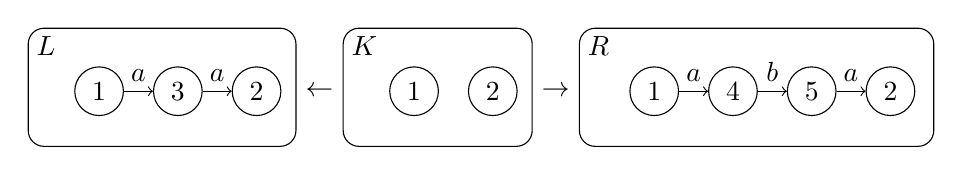
\begin{tikzpicture}[baseline=-10mm]
          \graphbox{$L$}{0mm}{0mm}{34mm}{15mm}{2mm}{-5mm}{
              \coordinate (o) at (0mm,-3mm); 
              \node[draw,circle] (l1) at ($(o)+(-10mm,0mm)$) {1};
              \node[draw,circle] (l2) at ($(l1)+(2,0)$) {2};
              \node[draw,circle] (l3) at ($(l1)+(1,0)$) {3};
              \draw[->] (l1) -- (l3) node[midway,above] {$a$};
              \draw[->] (l3) -- (l2) node[midway,above] {$a$};
          }     
          \graphbox{$K$}{40mm}{0mm}{24mm}{15mm}{2mm}{-5mm}{
              \coordinate (o) at (5mm,-3mm); 
              \node[draw,circle] (l1) at ($(o)+(-10mm,0mm)$) {1};
              \node[draw,circle] (l2) at ($(l1)+(1,0)$) {2};
              % \node[draw,circle] (l3) at ($(l1)+(1,0)$) {$\ $};
              % \draw[->] (l1) -- (l3) node[midway,above] {$a$};
              % \draw[->] (l3) -- (l2) node[midway,above] {$a$};
          }    
          \graphbox{$R$}{70mm}{0mm}{45mm}{15mm}{2mm}{-5mm}{
              \coordinate (o) at (-5mm,-3mm); 
              \node[draw,circle] (l1) at ($(o)+(-10mm,0mm)$) {1};
              \node[draw,circle] (l2) at ($(l1)+(3,0)$) {2};
              \node[draw,circle] (l3) at ($(l1)+(1,0)$) {4};
              \node[draw,circle] (l4) at ($(l1)+(2,0)$) {5};
              \draw[->] (l1) -- (l3) node[midway,above] {$a$};
              \draw[->] (l3) -- (l4) node[midway,above] {$b$};
              \draw[->] (l4) -- (l2) node[midway,above] {$a$};
          }    
          \node () at (37mm,-8mm) {$\leftarrow$};
          \node () at (67mm,-8mm) {$\rightarrow$};
          % \draw[>->] (51mm,2mm) -- (52mm,3mm);
      \end{tikzpicture}
      }
  \end{center}

  Weighted type graph $T$ over
    natural numbers:
 
   \begin{center}
        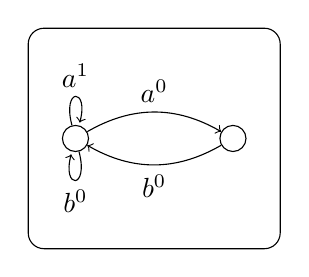
\begin{tikzpicture}
            \graphbox{}{0mm}{0mm}{32mm}{28mm}{-10mm}{-14mm}{
                \node[draw,circle] (1) at (0,0) {};
                \node[draw,circle] (2) at (2,0) {};
                \draw[->] (1) edge[loop above] node[midway, above] {$a^{1}$} (1) ;
                \draw[->] (1) edge[loop below] node[midway, below] {$b^{0}$} (1) ;
                \draw[->] (1) edge[bend left] node[midway, above] {$a^{0}$}  (2)  ;
                \draw[->] (2) edge[bend left] node[midway, below] {$b^{0}$} (1)   ;
            }
        \end{tikzpicture}
    \end{center}
\end{frame}

\begin{frame}{Intuition}
     \begin{itemize}
        \item $T$ : a weighted type graph 
        \item   \begin{flalign*}
                    G &\Longrightarrow \mathcal{F}(G,T)
                        \\
                    &\Longrightarrow \{weight(h) \mid h\in \mathcal{F}(G,T)\} 
                    \\
                    &\Longrightarrow \opn{agregateur}(\{weight(h) \mid h\in \mathcal{F}(G,T)\}) \in \mathbb{N}
                \end{flalign*}
     \end{itemize}
     Questions: 
     \begin{itemize}
        \item what is the weight of a morphism?
        \item which agregateur to use?
        \item How to approximate the weight of $G$ and $H$ in a rewriting step $G \Rightarrow H$ ?
     \end{itemize}
\end{frame}

\begin{frame}{Morphism weight}
    \begin{beamercolorbox}[wd=\textwidth,sep=1.2ex]{block body}
      The weight of a morphism $h: G \rightarrow T$ is \[\sum_{e \in \opn{Edge(G)}}\mathop{weight}(h(e)) \]
    \end{beamercolorbox}
    \resizebox{0.8\textwidth}{!}{
        \begin{tikzpicture}
          \graphbox{}{-50mm}{0mm}{40mm}{39mm}{2mm}{-6mm}{
            \coordinate (o) at (0mm,-10mm); 
            \node[draw,circle] (l1) at ($(o)+(-10mm,0mm)$) {1};
            \node[draw,circle] (l2) at ($(l1)+(2,0)$) {2};
            \node[draw,circle] (l3) at ($(l1)+(1,0)$) {3};
            \draw[red,->] (l1) -- (l3) node[midway,above] {$a$};
            \draw[red,->] (l3) -- (l2) node[midway,above] {$b$};
        } 
            \graphbox{$T$}{0mm}{0mm}{40mm}{39mm}{-10mm}{-17mm}{
                \node[draw,circle] (1) at (0,0) {$1\ 2$};
                \node[draw,circle] (2) at (2,0) {3};
                \draw[->] (1) edge[loop above] node[midway, above] {$a^{1}$} (1);
                \draw[->] (1) edge[loop below] node[midway, below] {$b^{0}$} (1);
                \draw[->,red] (1) edge[bend left] node[midway, above] {$a^{0}$}  (2);
                \draw[->,red] (2) edge[bend left] node[midway, below] {$b^{0}$} (1);
            }
            \node () at (-5mm,-15mm) {$\overset{h}{\to}$};
        \end{tikzpicture}
        }

        $ \opn{weight}_T(h) \mathop{=} 0 + 0 \mathop{=} 0$

\end{frame}
 

\begin{frame}{Graph weight} 
    \begin{beamercolorbox}[wd=\textwidth,sep=1.2ex]{block body}
        The weight of a graph $L$ is \[\min_{h : L \mathop{\to} T}  \opn{weight}_T(h)\]
    \end{beamercolorbox}
\begin{center}
    \resizebox{0.3\textwidth}{!}{
        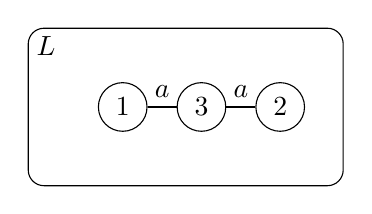
\begin{tikzpicture}
            \graphbox{\(L\)}{0mm}{0mm}{40mm}{20mm}{2mm}{0mm}{
                \coordinate (o) at (0mm,-10mm); 
                \node[draw,circle] (l1) at ($(o)+(-10mm,0mm)$) {1};
                \node[draw,circle] (l2) at ($(l1)+(2,0)$) {2};
                \node[draw,circle] (l3) at ($(l1)+(1,0)$) {3};
                \draw[] (l1) -- (l3) node[midway,above] {$a$};
                \draw[] (l3) -- (l2) node[midway,above] {$a$};
            } 
        \end{tikzpicture}
    }
\end{center}
Two morphisms from $L$ to $T$:
\begin{center}
      \resizebox{0.3\textwidth}{!}{
          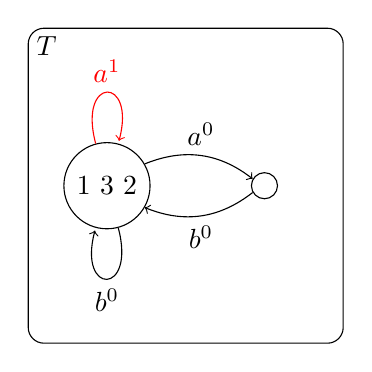
\begin{tikzpicture}
              \graphbox{$T$}{0mm}{0mm}{40mm}{40mm}{-10mm}{-20mm}{
                  \node[draw,circle] (1) at (0,0) {$1\ 3\ 2$};
                  \node[draw,circle] (2) at (2,0) {};
                  \draw[->,red] (1) edge[loop above] node[midway, above] {$a^{1}$} (1) ;
                  \draw[->] (1) edge[loop below] node[midway, below] {$b^{0}$} (1) ;
                  \draw[->] (1) edge[bend left] node[midway, above] {$a^{0}$}  (2)  ;
                  \draw[->] (2) edge[bend left] node[midway, below] {$b^{0}$} (1)   ;(1)   ;
              }
          \end{tikzpicture}
          }
        \resizebox{0.3\textwidth}{!}{
        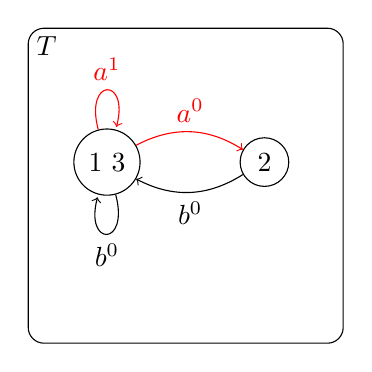
\begin{tikzpicture}
            \graphbox{$T$}{0mm}{0mm}{40mm}{40mm}{-10mm}{-17mm}{
                \node[draw,circle] (1) at (0,0) {$1\ 3$};
                \node[draw,circle] (2) at (2,0) {$2$};
                \draw[->,red] (1) edge[loop above] node[midway, above] {$a^{1}$} (1) ;
                \draw[->] (1) edge[loop below] node[midway, below] {$b^{0}$} (1) ;
                \draw[->,red] (1) edge[bend left] node[midway, above] {$a^{0}$}  (2)  ;
                \draw[->] (2) edge[bend left] node[midway, below] {$b^{0}$} (1)   ;
            }
        \end{tikzpicture}
        }
\end{center}

        $\opn{weight}_T(L) \mathop{=} \min \{1+1, 1+0\}\mathop{=} 1$       
\end{frame}

% \begin{frame}
%     \begin{center}
%         \resizebox{0.3\textwidth}{!}{
%             \begin{tikzpicture}
%             \graphbox{$R$}{0mm}{0mm}{45mm}{15mm}{2mm}{-10mm}{
%                 \coordinate (o) at (-5mm,0mm); 
%                 \node[draw,circle] (l1) at ($(o)+(-10mm,0mm)$) {1};
%                 \node[draw,circle] (l2) at ($(l1)+(3,0)$) {2};
%                 \node[draw,circle] (l3) at ($(l1)+(1,0)$) {4};
%                 \node[draw,circle] (l4) at ($(l1)+(2,0)$) {5};
%                 \draw[->] (l1) -- (l3) node[midway,above] {$a$};
%                 \draw[->] (l3) -- (l4) node[midway,above] {$b$};
%                 \draw[->] (l4) -- (l2) node[midway,above] {$a$};
%             } 
%             \end{tikzpicture}
%         }
%     \end{center}
%     has three morphisms to $T$:
%         \newline
%         \begin{center}
%             \resizebox{0.3\textwidth}{!}{
%                 \begin{tikzpicture}
%                     \graphbox{$T$}{0mm}{0mm}{45mm}{50mm}{-10mm}{-25mm}{
%                         \node[draw,circle] (1) at (0,0) {$1\ 2\ 4\ 5$};
%                         \node[draw,circle] (2) at (2,0) {};
%                         \draw[->,red] (1) edge[loop above] node[midway, above] {$a^{1}$} (1) ;
%                         \draw[->,red] (1) edge[loop below] node[midway, below] {$b^{0}$} (1);
%                         \draw[->] (1) edge[bend left] node[midway, above] {$a^{0}$}  (2);
%                         \draw[->] (2) edge[bend left] node[midway, below] {$b^{0}$} (1);
%                     }
%                 \end{tikzpicture}
%                 }
%             \resizebox{0.3\textwidth}{!}{
%             \begin{tikzpicture}
%                 \graphbox{$T$}{0mm}{0mm}{45mm}{50mm}{-10mm}{-25mm}{
%                     \node[draw,circle] (1) at (0,0) {$1\ 2\ 5$};
%                     \node[draw,circle] (2) at (2,0) {$4$};
%                     \draw[->,red] (1) edge[loop above] node[midway, above] {$a^{1}$} (1) ;
%                     \draw[->] (1) edge[loop below] node[midway, below] {$b^{0}$} (1) ;
%                     \draw[->,red] (1) edge[bend left] node[midway, above] {$a^{0}$}  (2)  ;
%                     \draw[->,red] (2) edge[bend left] node[midway, below] {$b^{0}$} (1);
%                 }
%             \end{tikzpicture}
%             }
%             \resizebox{0.3\textwidth}{!}{
%                 \begin{tikzpicture}
%                     \graphbox{$T$}{0mm}{0mm}{45mm}{50mm}{-10mm}{-25mm}{
%                         \node[draw,circle] (1) at (0,0) {$1\ 5$};
%                         \node[draw,circle] (2) at (2,0) {$4\ 2$};
%                         \draw[->] (1) edge[loop above] node[midway, above] {$a^{1}$} (1) ;
%                         \draw[->] (1) edge[loop below] node[midway, below] {$b^{0}$} (1) ;
%                         \draw[->,red] (1) edge[bend left] node[midway, above] {$a^{0}$}  (2)  ;
%                         \draw[->,red] (2) edge[bend left] node[midway, below] {$b^{0}$} (1);
%                     }
%                 \end{tikzpicture}
%             }
%     \end{center}

      
%      $\opn{weight}_T(R) = \min \{1+0+1, 0+0+1, 0 + 0 + 0\}\mathop{=} 0$.
% \end{frame}

% \begin{frame}
%   Since for all $G \mathop{\Rightarrow}_\alpha H$, we have $w_T(G) \mathop{\in} \mathbb{N}$, it remains to show that every rewriting step strictly decreases the weight.
% %   Not every weighted graph can be a weighted type graph
% %   It guarantees: for all $G \mathop{\Rightarrow}_\alpha H$, the weight of $G$ is defined and $w_T(G) \mathop{\in} \mathbb{N}$
% \end{frame}

% \begin{frame}{Condition on Weighted Type Graph: for every rewriting step $G \mathop{\Rightarrow} H$, there exists a morphism $h : G \mathop{\to} T$.}
  

%   Consequence: for all $G \mathop{\Rightarrow} H$, $G$ has a weight and $w(G) \mathop{\geq} 0$.
%   % \begin{definition}
%   %   % Let $T \mathop{=} (T,\mathbb{E}, S, w)$ be a type graph, \(\rho \mathop{=} (L \xleftarrow{l} K \xrightarrow{r} R ) \) a DPO rewriting rule and $\mathfrak{F}$ a rewriting framework. 
%   %   A \textbf{context closure} for a rule $\rho$ and a $T$ is a morphism $c:L \mathop{\rightarrow} T$ such that for every possible DPO diagram depicted below,
%   %   there exists $\alpha : G \mathop{\rightarrow} T$ such that $m \mathop{\star} \alpha \mathop{=} c$.
%   %   \begin{center}
%   %       \begin{tikzpicture}[rotate=90]
%   %         \node (I) {$K$}; 
%   %         \node (L) [left of=I] {$L$};
%   %         \node (R) [right of=I] {$R$};
%   %         \node (G) [below of=L] {$G$};
%   %         \node (C) [below of=I] {$C$};
%   %         \node (H) [below of=R] {$H$};
%   %         \node (T) [left=of $(L)!0.5!(G)$] {$T$};
%   %         \draw [->] (L) to  node [label, above] {$c$}  (T);
%   %         \draw [->] (G) to  node [label, below] {$\alpha$} (T);
%   %         \draw [->] (I) to node [label, above] {$l$} (L);
%   %         \draw [->] (I) to node [label,above] {$r$} (R);
%   %         \draw [->] (L) to node [label, right] {$m$} (G);
%   %         \draw [->] (I) to (C);
%   %         \draw [->] (R) to (H);
%   %         \draw [->] (C) to (G);
%   %         \draw [->] (C) to (H);
%   %       \end{tikzpicture}
%   %     \end{center}
%   % \end{definition}
%   % Consequence:
% \end{frame}


% \begin{frame}{ 
%   every rewriting step strictly decreases the weight if:
%   % $w_T(G) \mathop{>} w_T(H)$ for every rewriting step $G \mathop{\Rightarrow}_\varphi H$ using rule $\varphi \mathop{=} L \xleftarrow{l} K \xrightarrow{r} R$ if
%   }
%   %  For $G \mathop{\Rightarrow} H$ defined by

%   %  \begin{center}
%   %     \resizebox{0.3\textwidth}{!}{
%   %       \begin{tikzpicture}
%   %           \node (I) at (0,0) {$K$};
%   %           \node (L) at (-2,0) {$L$};
%   %           \node (R) at (2,0) {$R$};
%   %           \node (G) at (-2,-2) {$G$};
%   %           \node (C) at (0,-2) {$C$};
%   %           \node (H) at (2,-2) {$H$};
%   %           \draw [->] (I) to  node [midway,below] {$l$} (L);
%   %           \draw [->] (I) to  node [midway,below] {$r$} (R);
%   %           \draw [->] (L) to node [midway,right] {$m$} (G);
%   %           \draw [->] (I) to node [midway,right] {$u$} (C);
%   %           \draw [->] (R) to node [midway,left] {$m'$} (H);
%   %           \draw [->] (C) to node [midway,above] {$l'$} (G);
%   %           \draw [->] (C) to node [midway,above] {$r'$} (H);
%   %           \node [at=($(I)!.5!(G)$)] {\normalfont PO};
%   %           \node [at=($(I)!.5!(H)$)] {\normalfont PO};
%   %         \end{tikzpicture}
%   %       }
%   % \end{center}
% % It suffices to show
% % \begin{theorem}
%   for every $t_K: K \mathop{\rightarrow} T$, 

% \begin{flalign*}
%   &\text{the sum of the weights of the morphisms $t_L$ that extend $t_K$} 
%   \\
%   &\mathop{\geq}
%   \\
%   &\text{the sum of the weights of the morphisms $t_R$ that extend $t_K$}
% \end{flalign*}

%  $$ \sum ( w_T \{t_L :L \mathop{\to} T \mathop{\mid} \text{$t_L$ extends $t_K$}\} )
%        -  \sum_{\substack{t_R: R \mathop{\rightarrow} T\\ t_K \mathop{=} t_R \circ r}}
%             w_T(t_R) \mathop{\geq} 0 $$ 

%     $$ \sum_{\substack{t_L: L \mathop{\rightarrow} T\\ t_K \mathop{=}  t_L \circ l }}
%         w_T(t_L) -  \sum_{\substack{t_R: R \mathop{\rightarrow} T\\ t_K \mathop{=} t_R \circ r}}
%             w_T(t_R) \mathop{\geq} 0 $$ 

% for some $t_K: K \mathop{\rightarrow} T$,
% $$ \sum_{\substack{t_L: L \mathop{\rightarrow} T\\ t_K \mathop{=} t_L \circ l}}
%         w_T(t_L) - \sum_{\substack{t_R: R \mathop{\rightarrow} T\\ t_K \mathop{=} t_R \circ r}}
%             w_T(t_R) \mathop{>} \delta $$ 
% for some $t_K: K \mathop{\rightarrow} T$,
% \begin{flalign*}
%   &\text{the sum of the weights of the morphisms $t_L$ that extend $t_K$} 
%   \\
%   &\mathop{>}
%   \\
%   &\text{the sum of the weights of the morphisms $t_R$ that extend $t_K$}
% \end{flalign*}
% % \end{theorem}   
% % then 
% %   \begin{center}
% %     $w_T(G) - w_T(H) \mathop{>} \delta$ for every rewriting step $G \mathop{\Rightarrow}_\varphi H$ using rule $\varphi$
% %   \end{center}
%   by \cite[Lemma 5.13]{endrullis2024generalized_arxiv_v2}.
%   % \resizebox{0.9\textwidth}{!}{
%   %   \begin{flalign*}
%   %     w_T(G) 
%   %         & \mathop{=} \sum_{t_K: K \mathop{\rightarrow} T} 
%   %         \left ( \sum_{\substack{t_C: C \mathop{\rightarrow} T\\ t_K \mathop{=} u \mathop{\star} t_C}}
%   %           w_T(t_C - u) \right ) 
%   %           \times
%   %         \left (\sum_{\substack{t_L: L \mathop{\rightarrow} T\\ t_K \mathop{=} t_L \circ l}}
%   %         w_T(t_L) \right )
%   %         \\
%   %     w_T(H) 
%   %         &  \mathop{\preceq} \sum_{t_K: K \mathop{\rightarrow} T} 
%   %         \left ( \sum_{\substack{t_C: C \mathop{\rightarrow} T\\ t_K \mathop{=} u \mathop{\star} t_C}}
%   %         w_T(t_C - u) \right ) 
%   %         \mathop{\times} 
%   %         \left ( \sum_{\substack{t_R: R \mathop{\rightarrow} T\\ t_K \mathop{=} t_R \circ r}}
%   %             w_T(t_R) \right ) \\
%   % \end{flalign*}
%   % }
% \end{frame}

\begin{frame}{Extension of a morphism}
      \begin{beamercolorbox}[wd=\textwidth,sep=1.2ex]{block body}
        \begin{tikzpicture}
            \node (k) at (0,0) {$K$};
            \node (l) at (-2,0) {$L$};
            \node (t) at (-2,-2) {$T$};
            \node (r) at (2,0) {$R$};
            \draw [->] (k) to  node [midway,above] {$l$} (l);
            \draw [->] (k) to  node [midway,above] {$r$} (r);
            \draw [->] (k) to  node [midway,right] {$t_K$} (t);
            \draw [->,dashed] (l) to node [midway,left] {$t_L$} (t);
        \end{tikzpicture}

        A morphism $t_L: L \mathop{\rightarrow} T$ extends $t_K$ if
        $t_K \mathop{=} t_L \circ l$.

          For every morphism $t_K: K \mathop{\rightarrow} T$, we define
        \begin{itemize}
        \item $S(t_K,L)$ : the minimum weight of the morphisms $t_L$ that extend $t_K$,
        \item $S(t_K,R)$ : similarly.
        \end{itemize}
      \end{beamercolorbox}
\end{frame}

\begin{frame}{Termination Condition}
%   \begin{center} 
%       \resizebox{0.9\textwidth}{!}{
%       \begin{tikzpicture}
%           \graphbox{$L$}{0mm}{0mm}{34mm}{15mm}{2mm}{-5mm}{
%               \coordinate (o) at (0mm,-3mm); 
%               \node[draw,circle] (l1) at ($(o)+(-10mm,0mm)$) {1};
%               \node[draw,circle] (l2) at ($(l1)+(2,0)$) {2};
%               \node[draw,circle] (l3) at ($(l1)+(1,0)$) {3};
%               \draw[->] (l1) -- (l3) node[midway,above] {$a$};
%               \draw[->] (l3) -- (l2) node[midway,above] {$a$};
%           }     
%           \graphbox{$K$}{40mm}{0mm}{24mm}{15mm}{2mm}{-5mm}{
%               \coordinate (o) at (5mm,-3mm); 
%               \node[draw,circle] (l1) at ($(o)+(-10mm,0mm)$) {1};
%               \node[draw,circle] (l2) at ($(l1)+(1,0)$) {2};
%               % \node[draw,circle] (l3) at ($(l1)+(1,0)$) {$\ $};
%               % \draw[->] (l1) -- (l3) node[midway,above] {$a$};
%               % \draw[->] (l3) -- (l2) node[midway,above] {$a$};
%           }    
%           \graphbox{$R$}{70mm}{0mm}{45mm}{15mm}{2mm}{-5mm}{
%               \coordinate (o) at (-5mm,-3mm); 
%               \node[draw,circle] (l1) at ($(o)+(-10mm,0mm)$) {1};
%               \node[draw,circle] (l2) at ($(l1)+(3,0)$) {2};
%               \node[draw,circle] (l3) at ($(l1)+(1,0)$) {4};
%               \node[draw,circle] (l4) at ($(l1)+(2,0)$) {5};
%               \draw[->] (l1) -- (l3) node[midway,above] {$a$};
%               \draw[->] (l3) -- (l4) node[midway,above] {$b$};
%               \draw[->] (l4) -- (l2) node[midway,above] {$a$};
%           }    
%           \node () at (37mm,-8mm) {$\overset{l}{\leftarrow}$};
%           \node () at (67mm,-8mm) {$\rightarrow$};
%           % \draw[>->] (51mm,2mm) -- (52mm,3mm);
%       \end{tikzpicture}
%       }
%   \end{center}
    \begin{corollary}[Bruggink et al. 2014~\cite{bruggink2014termination}]
        Every rewriting step strictly decreases the weight if 
        \begin{itemize}
        % \item for every $t_K: K \mathop{\rightarrow} T$, $$ S(t_K,L) \mathop{\geq} S(t_K,R) $$.
        \item for all $t_K: K \mathop{\rightarrow} T$, if there is a morphism $t_L$ that extends $t_K$, then 
        $$ S(t_K,L) \mathop{>} S(t_K,R) $$
        \end{itemize} 
    \end{corollary}

    How to find such a suitable weighted type graph ?
\end{frame}

% \subsection{Searching for suitable weighted type graphs in practice}

\begin{frame}{Searching for Weighted Type Graphs over Natural Numbers}
    User-specified parameters:
      \begin{itemize}
        \item $k$ nodes
        \item maximum edge weight $n\in\mathbb{N}$
      \end{itemize}   
    Assumption:
      \begin{itemize}
        \item no parallel edges of the same label 
      \end{itemize}
    The problem amounts to checking the \textcolor{red}{satisfiability of an
existential Presburger arithmetic theory} with:
                \begin{itemize}
                  \item $k^2m$ binary variables where $m$ is the number of labels
                  \item $k^2m$ integer variables
                \end{itemize} 
  Challenge:
  \begin{itemize}
    \item $2^{k^2m} \cdot n^{k^2m}$ possible assignments of weights
    \item maximum edge weight hard to determine to guess
  \end{itemize} 
\end{frame}

% \subsection{Accelerating the Search}

\begin{frame}{Solution: using real numbers instead of natural numbers.}
  
 Every rewriting step strictly decreases the weight if 
\begin{itemize}
  \item for all $t_K: K \mathop{\rightarrow} T$, if there is a morphism $t_L$ that extends $t_K$, then 
  $$ S(t_K,L) \mathop{>} S(t_K,R) $$
   \item there is $\delta > 0$ such that for all $t_K: K \mathop{\rightarrow} T$, if there is a morphism $t_L$ that extends $t_K$, then 
  $$ S(t_K,L) \mathop{>} S(t_K,R)\mathop{+}\delta$$
\end{itemize} 
\end{frame}


\begin{frame}{Searching for Weighted Type Graphs over Real Numbers}
    User-specified parameters:
      \begin{itemize}
        \item $k$ nodes
        \item \crossout[red]{edge weights in $\{0, 1, \ldots, n\}$}
      \end{itemize}   
    Assumption:
      \begin{itemize}
        \item no parallel edges of the same label 
      \end{itemize}
    The problem amounts to checking the satisfiability of an
\crossout[red]{existential Presburger arithmetic theory} \textcolor{blue}{existential theory of the reals with binary variables}:
                \begin{itemize}
                  \item $k^2m$ binary variables where $m$ is the number of labels
                  \item $k^2m$ \crossout[blue]{integer} \textcolor{red}{real} variables
                \end{itemize} 
  Challenge:
  \begin{itemize}
    \item \crossout[red]{there are $2^{k^2m} \cdot n^{k^2m}$ possible assignments of weights}
    \item there are $2^{k^2m}$ linear programs which have polynomial-time average-case complexity
  \end{itemize} 
\end{frame}

\begin{frame}{Experimental Results}
 
    \begin{table}[htb]   
        \renewcommand{\arraystretch}{1.2}
        \centering
        \begin{adjustbox}{max width=\textwidth,max totalheight=0.8\textheight,keepaspectratio}
    \begin{tabular}{|c|c|c|c|c|c|c |}
        \hline
        &\;\;A\;\;&\;\;a\;\;&\;\;T\;\;&\;\;t\;\;&\;\; N\;\;&\;\;n\;\; \\
        \hline
    % ~\cite[Example 6.2]{endrullis2024generalized_arxiv_v2} & & & & & 2.68 &1.15   \\
    ~\cite[Example 6.3]{endrullis2024generalized_arxiv_v2} & & & & & 2.74 &1.16   \\
        %~\cite[Example 6.4]{endrullis2024generalized_arxiv_v2}&  && & &  &   &  &  & our only Graph\\
    ~\cite[Example D.3]{endrullis2024generalized_arxiv_v2} &2.25 
        % (2.30+2.188+2.2637+2.2928+ 2.196) 
        & 1.18
        % (1.17+1.2549+1.165+ 1.1576\mathop{+}1.162)
        & & & 2.24& 1.18    \\
    ~\cite[Example 3.8]{plump1995ontermination}
    & 2.95& 1.90 & 2.94 &1.87  & 3.49  &1.87   \\
        %~\cite[Example 3]{plump2018modular}
        % & 3.45& 3.44 & 3.55 &2.38  & 3.96  &17.60 &   4.24 AT &  3.45 at& 4.07 t  \\
    ~\cite[Example 4]{plump2018modular} &4.26& 3.19&  4.24 & 3.13 &
        5.82
        % (5.77+5.83+5.775+5.84+5.818+5.89)
        & timeout  \\

    ~\cite[Example 5]{plump2018modular} & 5.54
        &5.55
        % (5.53 +5.660\mathop{+}5.5213+5.5369+5.484689\mathop{+}5.6404\mathop{+}5.4877\mathop{+}5.5026)
        & 5.53& 5.50& 9.11&  5.62  \\
    % ~\cite[Example 6]{plump2018modular} &  &  & & &  &   \\
        % (* en haut j'ai enverse tropical et arctic *)
        %~\cite[Example 6]{plump2018modular} &  &6.93 & 6.38 & 6.30 & 7.87&  7.22  &  11.71 at & 7.71 AT& 13.60 ATNat \\
    ~\cite[Example 4]{bruggink2015proving} &
        2.44
        % (2.4415+ 2.4181+2.4466+2.4366+2.4624+2.4479)
        & 
        2.46
        % (2.4405+2.5180+2.4137+2.4539+2.4480+2.4750)
        & 
        2.47
        % (2.4660+2.4457+2.4559+2.4526+2.4588+2.4847+2.5731)/7
        &
        2.54
        % (2.4380+2.4557+2.5590+2.5631+2.7245+2.5041+2.5182)/7
        & 4.58 & 
        2.46
        % (2.3987+2.4521+2.4620+2.4558+2.5128+2.4507)/6
        \\
    ~\cite[Example 5]{bruggink2015proving} &  &  &&& 7.80& timeout  \\
    ~\cite[Example 6]{bruggink2015proving} &  &  &&& 9.75& timeout   \\
    ~\cite[Example 1]{bruggink2014termination} & 
        2.26
        %  (2.2887\mathop{+}2.2386 +2.2719\mathop{+}2.2735 +2.3025\mathop{+}2.1925)/6
        &1.18
        %  (1.1764+1.1837+1.1709+1.2222+1.1608+1.1645)/6
        & & &2.24
        %  (2.2365+2.2388+2.2124+2.2395+2.2550+2.2513)/6
        & 1.18  
        %  (1.2498+1.1710+1.1634+1.1655+1.1687+1.1733)/6
        \\
    ~\cite[Example 4]{bruggink2014termination} &  2.25
        % (2.2545+2.2512+2.2529+2.3498+2.2137+ 2.2257\mathop{+}2.2167\mathop{+}2.2413)/8
        & 1.22 & 2.24
        % (2.2981+2.2026\mathop{+}2.2229+2.2524+2.2421+2.2415)/6
        &1.18
        % (1.1261+1.1850+1.1848+1.1706+1.2052+1.1920)/6
        &2.25
        % (2.2347+2.3106+2.2130+2.2391+2.2466+2.2493)/6 
        & 1.19 

        \\
    ~\cite[Example 5]{bruggink2014termination} &  4.23 & 3.23  & 4.25 &3.28  & 5.82 & timeout \\
        %~\cite[Example 6]{bruggink2014termination} &  2.58& 1.63 & 2.61&1.65&2.67 & 1.50 \\
        %~\cite[Routing]{bruggink2014termination} &  & & & & &    
        % \\
        %~\autoref{nonwf} with $n=3$ & - & 1.90 &-& 1.95 &- & 2.00 & - & 2.47 a & 3.56 nT  \\
        \hline
        \end{tabular}
    \end{adjustbox}
        % \caption{
        % ``A'', ``T'', ``N'' : different approaches with weights over the natural numbers.
        % ``a'', ``t'', ``n'' : corresponding approaches over the real numbers.
        % }
        % \label{tabular:benchmarks}
    \end{table}
     ``A'', ``T'', ``N'' : different configurations with weights over the natural numbers. 
        ``a'', ``t'', ``n'' : corresponding configurations over the real numbers.
\end{frame}
 
\begin{frame}{Analysis and Implementation choices}
    Observations from experiments:
    \begin{itemize}
        \item advantages:
            \begin{itemize}
                \item less time in average to find a suitable weighted type graph 
                \item no need to guess maximum edge weight
            \end{itemize}
        \item disadvantage:
            \begin{itemize}
                \item impossible to further constrain weight sets to extremely small sets (e.g. with two elements).
                % \item less efficient when weights are extremely small integers
            \end{itemize}
    \end{itemize}
    Implementation choices:
    \begin{itemize}
        \item search in parallel using all approaches
        \item Z3 for checking satisfiability
    \end{itemize}
\end{frame}

\section{Termination using Morphism Counting}
\begin{frame}
  \tableofcontents[currentsection,hideothersubsections]
\end{frame}


\begin{frame}{Inclusions : morphisms $h$ with $h(x) = x$ for all $x$.}
         \begin{center} 
            \resizebox{0.7\textwidth}{!}{
                \begin{tikzpicture}
                    \graphbox{$G$}{39mm}{0mm}{35mm}{40mm}{2mm}{-5mm}{
                        \coordinate (delta) at (0,-18mm);
                        \node[draw,circle,red] (l1) at ($(delta)+(-1,1.5)$) {1};
                        \node[draw,circle,red] (l2) at ($(delta)+(1,1.5)$) {2};
                        \node[draw,circle,red] (l3) at ($(delta)+(0,0)$) {3};
                        \draw[->,red] (l1) -- (l3) node[midway,left] {$s$};
                        \draw[->,red] (l2) -- (l3) node[midway,right] {$s$};
                        \draw[->,red] (l3) edge [loop below] node {0} (l3);
                    }
                        \node () at (77mm,-18mm) {$\overset{h}{\rightarrow}$};
                    \graphbox{$H$}{80mm}{0mm}{50mm}{40mm}{2mm}{-5mm}{
                        \coordinate (delta) at (-10mm,-18mm);
                        \node[draw,circle,red] (r1) at ($(delta)+(-1,1.5)$) {1};
                        \node[draw,circle,red] (r2) at ($(delta)+(0.5,1.5)$) {2};
                        \node[draw,circle,red] (r3) at ($(delta)+(0,0)$) {3};
                        \node[draw,circle] (r4) at ($(delta)+(1,0)$) {};
                        \node[draw,circle] (r5) at ($(r2)+(1.5,0)$) {};
                        \draw[->] (r1) edge[bend right] node[midway,left] {$s$} (r3) ; 
                        \draw[->] (r2) -- (r4) node[midway,right] {$s$};
                        \draw[->] (r4) edge [loop below] node {0} (r4);
                        \draw[->] (r5) edge [loop below] node {0} (r5);
                        \draw[->] (r5) edge [loop right] node {0} (r5);
                        \draw[->] (r5) edge [loop left] node {0} (r5);
                        \draw[->,red] (r1) edge node[midway,left] {$s$} (r3) ;
                        \draw[->,red] (r2) edge node[midway,right] {$s$} (r3) ; 
                        \draw[->,red] (r3) edge [loop below] node {0} (r3); 
                    }
                \end{tikzpicture}
                }
        \end{center}
    Remarks:
        \begin{itemize}
            \item $G$ is a subgraph of $H$.
        \end{itemize}
\end{frame}

\begin{frame}{Graph rewriting rule}
      \begin{beamercolorbox}[wd=\textwidth,sep=1.2ex]{block body}
        \textcolor{red}{Rules} $\varphi \mathop{=} (L \overset{l}{\leftarrow} K \overset{r}{\rightarrow} R)$ consist of inclusions $l$ and $r$. 
      \end{beamercolorbox}
    \begin{center} 
        \resizebox{0.9\textwidth}{!}{
        $\alpha$ = 
        \begin{tikzpicture}[baseline=-10mm]
            \graphbox{\( L \)}{0mm}{-3mm}{34mm}{12mm}{2mm}{2mm}{
                \coordinate (o) at (0mm,-8mm); 
                \node[draw,circle] (l1) at ($(o)+(-10mm,0mm)$) {1};
                \node[draw,circle] (l2) at ($(l1)+(2,0)$) {2};
                \node[draw,circle] (l3) at ($(l1)+(1,0)$) {3};
                \draw[->] (l1) -- (l3) node[midway,above] {$a$};
                \draw[->] (l3) -- (l2) node[midway,above] {$a$};
            } 

            \graphbox{\( K \)}{40mm}{-3mm}{34mm}{12mm}{2mm}{2mm}{
                \coordinate (o) at (0mm,-8mm); 
                \node[draw,circle] (l1) at ($(o)+(-10mm,0mm)$) {1};
                \node[draw,circle] (l2) at ($(l1)+(2,0)$) {2};
            }  

            \graphbox{\( R \)}{80mm}{-3mm}{45mm}{12mm}{2mm}{2mm}{
                \coordinate (o) at (-5mm,-8mm); 
                \node[draw,circle] (l1) at ($(o)+(-10mm,0mm)$) {1};
                \node[draw,circle] (l2) at ($(l1)+(3,0)$) {2};
                \node[draw,circle] (l3) at ($(l1)+(1,0)$) {4};
                \node[draw,circle] (l4) at ($(l1)+(2,0)$) {5};
                \draw[->] (l1) -- (l3) node[midway,above] {$a$};
                \draw[->] (l3) -- (l4) node[midway,above] {$b$};
                \draw[->] (l4) -- (l2) node[midway,above] {$a$};
            }    
            \node () at (37mm,-8mm) {\( \overset{l}{\leftarrow} \)}; % K -> L
            \node () at (77mm,-8mm) {\( \overset{r}{\rightarrow} \)}; % K -> R
        \end{tikzpicture}
        } 
    \end{center}   
% to do todo
        \begin{beamercolorbox}[wd=\textwidth,sep=1.2ex]{block body}
            Rule $\varphi' \mathop{=} (L' \overset{l'}{\leftarrow} K' \overset{r'}{\rightarrow} R')$ and $\varphi$ are \alert{equivalent} if 
            there are isomorphisms $a,b,c$ such that:
            \begin{center}
                    \resizebox{0.40\textwidth}{!}{
                        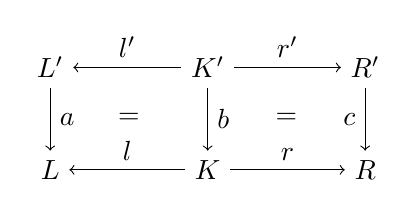
\begin{tikzpicture}
                                \node (I) at (0,-0.7) {$K'$};
                                \node (L) at (-2,-0.7) {$L'$};
                                \node (R) at (2,-0.7) {$R'$};
                                \node (G) at (-2,-2) {$L$};
                                \node (C) at (0,-2) {$K$};
                                \node (H) at (2,-2) {$R$};
                                \draw [->] (I) to  node [midway,above] {$l'$} (L);
                                \draw [->] (I) to  node [midway,above] {$r'$} (R);
                                \draw [->] (L) to node [midway,right] {$a$} (G);
                                \draw [->] (I) to node [midway,right] {$b$} (C);
                                \draw [->] (R) to node [midway,left] {$c$} (H);
                                \draw [->] (C) to node [midway,above] {$l$} (G);
                                \draw [->] (C) to node [midway,above] {$r$} (H);
                                \node [at=($(I)!.5!(G)$)] {=};
                                \node [at=($(I)!.5!(H)$)] {=};
                            \end{tikzpicture}
                    }
                \end{center}
        \end{beamercolorbox}
    \begin{center}
     \resizebox{0.9\textwidth}{!}{
        $\alpha'$ = 
           \begin{tikzpicture}[baseline=-10mm]
                \graphbox{\( L' \)}{0mm}{-3mm}{34mm}{12mm}{2mm}{2mm}{
                    \coordinate (o) at (0mm,-8mm); 
                    \node[draw,circle] (l1) at ($(o)+(-10mm,0mm)$) {6};
                    \node[draw,circle] (l2) at ($(l1)+(2,0)$) {8};
                    \node[draw,circle] (l3) at ($(l1)+(1,0)$) {7};
                    \draw[->] (l1) -- (l3) node[midway,above] {$a$};
                    \draw[->] (l3) -- (l2) node[midway,above] {$a$};
                } 
        
                \graphbox{\( K' \)}{40mm}{-3mm}{34mm}{12mm}{2mm}{2mm}{
                    \coordinate (o) at (0mm,-8mm); 
                    \node[draw,circle] (l1) at ($(o)+(-10mm,0mm)$) {6};
                    \node[draw,circle] (l2) at ($(l1)+(2,0)$) {7};
                }  
        
                \graphbox{\( R' \)}{80mm}{-3mm}{45mm}{12mm}{2mm}{2mm}{
                    \coordinate (o) at (-5mm,-8mm); 
                    \node[draw,circle] (l1) at ($(o)+(-10mm,0mm)$) {6};
                    \node[draw,circle] (l2) at ($(l1)+(3,0)$) {7};
                    \node[draw,circle] (l3) at ($(l1)+(1,0)$) {9};
                    \node[draw,circle] (l4) at ($(l1)+(2,0)$) {10};
                    \draw[->] (l1) -- (l3) node[midway,above] {$a$};
                    \draw[->] (l3) -- (l4) node[midway,above] {$b$};
                    \draw[->] (l4) -- (l2) node[midway,above] {$a$};
                }    
                \node () at (37mm,-8mm) {\( \overset{l'}{\leftarrow} \)};  
                \node () at (77mm,-8mm) {\( \overset{r'}{\rightarrow} \)}; %
            \end{tikzpicture}
            }     
    \end{center}    
\end{frame}

\begin{frame}{Graph Rewriting}
 
 Rewriting steps $G \mathop{\Rightarrow}_\varphi H$ using rule $\varphi$ are commutative diagrams with an equivalent rule $L' \overset{l'}{\leftarrow} K' \overset{r'}{\rightarrow} R'$ where all morphisms are inclusions:
         \begin{center}
          \resizebox{0.40\textwidth}{!}{
              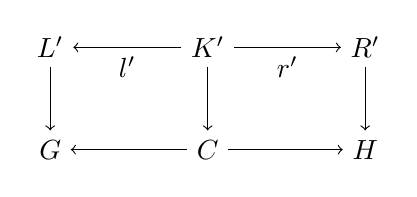
\begin{tikzpicture}
                    \node (I) at (0,-0.7) {$K'$};
                    \node (L) at (-2,-0.7) {$L'$};
                    \node (R) at (2,-0.7) {$R'$};
                    \node (G) at (-2,-2) {$G$};
                    \node (C) at (0,-2) {$C$};
                    \node (H) at (2,-2) {$H$};
                    \draw [->] (I) to  node [midway,below] {$l'$} (L);
                    \draw [->] (I) to  node [midway,below] {$r'$} (R);
                    \draw [->] (L) to node [midway,left] {} (G);
                    \draw [->] (I) to node [midway,right] { } (C);
                    \draw [->] (R) to node [midway,left] { } (H);
                    \draw [->] (C) to node [midway,above] { } (G);
                    \draw [->] (C) to node [midway,above] { } (H);
                    \node [at=($(I)!.5!(G)$)] {} ;
                    \node [at=($(I)!.5!(H)$)] {};
                  \end{tikzpicture}
          }
      \end{center}

%       A rewriting step using $\varphi$:
%   \begin{center}
%     \resizebox{0.7\textwidth}{!}{
%       \begin{tikzpicture}
%               \graphbox{\( L\)}{0mm}{5mm}{34mm}{20mm}{2mm}{-5mm}{
%                   \coordinate (o) at (0mm,-8mm); 
%                   \node[draw,circle] (l1) at ($(o)+(-10mm,0mm)$) {1};
%                   \node[draw,circle] (l2) at ($(l1)+(2,0)$) {2};
%                   \node[orange,draw,circle] (l3) at ($(l1)+(1,0)$) {3};
%                   \draw[orange,->] (l1) -- (l3) node[midway,above] {$a$};
%                   \draw[orange,->] (l3) -- (l2) node[midway,above] {$a$};
%               } 

%               \graphbox{\( K \)}{40mm}{5mm}{34mm}{20mm}{2mm}{-5mm}{
%                   \coordinate (o) at (0mm,-8mm); 
%                   \node[draw,circle] (l1) at ($(o)+(-10mm,0mm)$) {1};
%                   \node[draw,circle] (l2) at ($(l1)+(2,0)$) {2};
%               }  

%               \graphbox{\( R \)}{80mm}{5mm}{45mm}{20mm}{2mm}{-5mm}{
%                   \coordinate (o) at (-5mm,-8mm); 
%                   \node[draw,circle] (l1) at ($(o)+(-10mm,0mm)$) {1};
%                   \node[draw,circle] (l2) at ($(l1)+(3,0)$) {2};
%                   \node[red,draw,circle] (l3) at ($(l1)+(1,0)$) {4};
%                   \node[red,draw,circle] (l4) at ($(l1)+(2,0)$) {5};
%                   \draw[red,->] (l1) -- (l3) node[midway,above] {$a$};
%                   \draw[red,->] (l3) -- (l4) node[midway,above] {$b$};
%                   \draw[red,->] (l4) -- (l2) node[midway,above] {$a$};
%               }    

%               \graphbox{\( G  \)}{0mm}{-22mm}{34mm}{30mm}{2mm}{-10mm}{
%                   \coordinate (o) at (0mm,-3mm); 
%                   \node[draw,circle] (l1) at ($(o)+(-10mm,0mm)$) {1};
%                   \node[draw,circle] (l2) at ($(l1)+(2,0)$) {2};
%                   \node[draw,circle,orange] (l3) at ($(l1)+(1,0)$) {3};
%                   \node[blue, draw,circle] (l4) at ($(l2)+(0,-1)$) {6};
%                   \draw[orange,->] (l1) -- (l3) node[midway,above] {$a$};
%                   \draw[orange,->] (l3) -- (l2) node[midway,above] {$a$};
%                   \draw[blue,->] (l2) -- (l4) node[midway,right] {$a$};
%                 %   \node[blue,draw,circle] (l6) at ($(l1)+(0,-1)$) {7};
%                 %   \draw[blue,<-] (l1) -- (l6) node[midway,left] {$a$};
%               }    

%               \graphbox{\( C  \)}{40mm}{-22mm}{34mm}{30mm}{2mm}{-10mm}{
%                   \coordinate (o) at (0mm,-3mm); 
%                   \node[draw,circle] (l1) at ($(o)+(-10mm,0mm)$) {1};
%                   \node[draw,circle] (l2) at ($(l1)+(2,0)$) {2};
%                   \node[blue,draw,circle] (l4) at ($(l2)+(0,-1)$) {6};
%                   \draw[blue,->] (l2) -- (l4) node[midway,right] {$a$};
%                 %   \node[blue,draw,circle] (l6) at ($(l1)+(0,-1)$) {7};
%                 %   \draw[blue,<-] (l1) -- (l6) node[midway,left] {$a$};
%               }    

%               \graphbox{\( H   \)}{80mm}{-22mm}{45mm}{30mm}{2mm}{-10mm}{
%                   \coordinate (o) at (-5mm,-3mm); 
%                   \node[draw,circle] (l1) at ($(o)+(-10mm,0mm)$) {1};
%                   \node[draw,circle] (l2) at ($(l1)+(3,0)$) {2};
%                   \node[draw,circle,red] (l3) at ($(l1)+(1,0)$) {4};
%                   \node[draw,circle,red] (l4) at ($(l1)+(2,0)$) {5};
%                   \node[blue,draw,circle] (l5) at ($(l2)+(0,-1)$) {6};
%                 %   \node[blue,draw,circle] (l6) at ($(l1)+(0,-1)$) {7};
%                 %   \draw[blue,<-] (l1) -- (l6) node[midway,left] {$a$};
%                   \draw[red,->] (l1) -- (l3) node[midway,above] {$a$};
%                   \draw[red,->] (l3) -- (l4) node[midway,above] {$b$};
%                   \draw[red,->] (l4) -- (l2) node[midway,above] {$a$};
%                   \draw[blue,->] (l2) -- (l5) node[midway,right] {$a$};
%               }    

%               \node () at (37mm,-8mm) {\( \overset{l}{\leftarrow} \)}; % K -> L
%               \node () at (77mm,-8mm) {\( \overset{r}{\rightarrow} \)}; % K -> R
%               \node () at (17mm,-18mm) {\( \downarrow \)};
%               \node () at (37mm,-33mm) {\( \leftarrow \)};
%               \node () at (52mm,-18mm) {\( \downarrow \)};
%               \node () at (92mm,-18mm) {\( \downarrow \)};
%               \node () at (77mm,-33mm) {\( \rightarrow \)}; % C -> H
%       \end{tikzpicture}
%       }
%    \end{center}
\end{frame} 
 
\begin{frame}{A rewriting step with a running example}
  Rewriting rule:
  \begin{center}
    $\varphi$=\resizebox{0.78\textwidth}{!}{
      \begin{tikzpicture}[baseline=-10mm]
              \graphbox{\( L\)}{0mm}{5mm}{34mm}{15mm}{2mm}{0mm}{
                  \coordinate (o) at (0mm,-8mm); 
                  \node[draw,circle] (l1) at ($(o)+(-10mm,0mm)$) {6};
                  \node[draw,circle] (l2) at ($(l1)+(2,0)$) {7};
                  \node[orange,draw,circle] (l3) at ($(l1)+(1,0)$) {8};
                  \draw[orange,->] (l1) -- (l3) node[midway,above] {$a$};
                  \draw[orange,->] (l3) -- (l2) node[midway,above] {$a$};
              } 

              \graphbox{\( K \)}{40mm}{5mm}{34mm}{15mm}{2mm}{0mm}{
                  \coordinate (o) at (0mm,-8mm); 
                  \node[draw,circle] (l1) at ($(o)+(-10mm,0mm)$) {6};
                  \node[draw,circle] (l2) at ($(l1)+(2,0)$) {7};
              }  

              \graphbox{\( R \)}{80mm}{5mm}{45mm}{15mm}{2mm}{0mm}{
                  \coordinate (o) at (-5mm,-8mm); 
                  \node[draw,circle] (l1) at ($(o)+(-10mm,0mm)$) {6};
                  \node[draw,circle] (l2) at ($(l1)+(3,0)$) {7};
                  \node[red,draw,circle] (l3) at ($(l1)+(1,0)$) {9};
                  \node[red,draw,circle] (l4) at ($(l1)+(2,0)$) {10};
                  \draw[red,->] (l1) -- (l3) node[midway,above] {$a$};
                  \draw[red,->] (l3) -- (l4) node[midway,above] {$b$};
                  \draw[red,->] (l4) -- (l2) node[midway,above] {$a$};
              }    
              \node () at (37mm,-3mm) {\( \overset{l}{\leftarrow} \)}; % K -> L
              \node () at (77mm,-3mm) {\( \overset{r}{\rightarrow} \)}; % K -> R
      \end{tikzpicture}
      }
   \end{center}

   An equivalent rewriting rule:
  \begin{center}
    $\varphi'$=\resizebox{0.78\textwidth}{!}{
      \begin{tikzpicture}[baseline=-10mm]
              \graphbox{\( L' \)}{0mm}{5mm}{34mm}{15mm}{2mm}{0mm}{
                  \coordinate (o) at (0mm,-8mm); 
                  \node[draw,circle] (l1) at ($(o)+(-10mm,0mm)$) {1};
                  \node[draw,circle] (l2) at ($(l1)+(2,0)$) {2};
                  \node[orange,draw,circle] (l3) at ($(l1)+(1,0)$) {3};
                  \draw[orange,->] (l1) -- (l3) node[midway,above] {$a$};
                  \draw[orange,->] (l3) -- (l2) node[midway,above] {$a$};
              } 

              \graphbox{\( K' \)}{40mm}{5mm}{34mm}{15mm}{2mm}{0mm}{
                  \coordinate (o) at (0mm,-8mm); 
                  \node[draw,circle] (l1) at ($(o)+(-10mm,0mm)$) {1};
                  \node[draw,circle] (l2) at ($(l1)+(2,0)$) {2};
              }  

              \graphbox{\( R' \)}{80mm}{5mm}{45mm}{15mm}{2mm}{0mm}{
                  \coordinate (o) at (-5mm,-8mm); 
                  \node[draw,circle] (l1) at ($(o)+(-10mm,0mm)$) {1};
                  \node[draw,circle] (l2) at ($(l1)+(3,0)$) {2};
                  \node[red,draw,circle] (l3) at ($(l1)+(1,0)$) {4};
                  \node[red,draw,circle] (l4) at ($(l1)+(2,0)$) {5};
                  \draw[red,->] (l1) -- (l3) node[midway,above] {$a$};
                  \draw[red,->] (l3) -- (l4) node[midway,above] {$b$};
                  \draw[red,->] (l4) -- (l2) node[midway,above] {$a$};
              }    
              \node () at (37mm,-3mm) {\( \overset{l'}{\leftarrow} \)}; 
              \node () at (77mm,-3mm) {\( \overset{r'}{\rightarrow} \)}; 
      \end{tikzpicture}
      }
   \end{center}
  
   A rewriting step $G \Rightarrow_\varphi H$:
  \begin{center}
    \resizebox{0.78\textwidth}{!}{
      \begin{tikzpicture}
              \graphbox{\( L' \)}{0mm}{5mm}{34mm}{15mm}{2mm}{0mm}{
                  \coordinate (o) at (0mm,-8mm); 
                  \node[draw,circle] (l1) at ($(o)+(-10mm,0mm)$) {1};
                  \node[draw,circle] (l2) at ($(l1)+(2,0)$) {2};
                  \node[orange,draw,circle] (l3) at ($(l1)+(1,0)$) {3};
                  \draw[orange,->] (l1) -- (l3) node[midway,above] {$a$};
                  \draw[orange,->] (l3) -- (l2) node[midway,above] {$a$};
              } 

              \graphbox{\( K' \)}{40mm}{5mm}{34mm}{15mm}{2mm}{0mm}{
                  \coordinate (o) at (0mm,-8mm); 
                  \node[draw,circle] (l1) at ($(o)+(-10mm,0mm)$) {1};
                  \node[draw,circle] (l2) at ($(l1)+(2,0)$) {2};
              }  

              \graphbox{\( R' \)}{80mm}{5mm}{45mm}{15mm}{2mm}{0mm}{
                  \coordinate (o) at (-5mm,-8mm); 
                  \node[draw,circle] (l1) at ($(o)+(-10mm,0mm)$) {1};
                  \node[draw,circle] (l2) at ($(l1)+(3,0)$) {2};
                  \node[red,draw,circle] (l3) at ($(l1)+(1,0)$) {4};
                  \node[red,draw,circle] (l4) at ($(l1)+(2,0)$) {5};
                  \draw[red,->] (l1) -- (l3) node[midway,above] {$a$};
                  \draw[red,->] (l3) -- (l4) node[midway,above] {$b$};
                  \draw[red,->] (l4) -- (l2) node[midway,above] {$a$};
              }    
                \graphbox{\( G  \)}{0mm}{-17mm}{34mm}{25mm}{2mm}{-5mm}{
                  \coordinate (o) at (0mm,-3mm); 
                  \node[draw,circle] (l1) at ($(o)+(-10mm,0mm)$) {1};
                  \node[draw,circle] (l2) at ($(l1)+(2,0)$) {2};
                  \node[draw,circle,orange] (l3) at ($(l1)+(1,0)$) {3};
                  \node[blue, draw,circle] (l4) at ($(l2)+(0,-1)$) {6};
                  \draw[orange,->] (l1) -- (l3) node[midway,above] {$a$};
                  \draw[orange,->] (l3) -- (l2) node[midway,above] {$a$};
                  \draw[blue,->] (l2) -- (l4) node[midway,right] {$a$};
              }    
              \graphbox{\( C  \)}{40mm}{-17mm}{34mm}{25mm}{2mm}{-5mm}{
                  \coordinate (o) at (0mm,-3mm); 
                  \node[draw,circle] (l1) at ($(o)+(-10mm,0mm)$) {1};
                  \node[draw,circle] (l2) at ($(l1)+(2,0)$) {2};
                  \node[blue,draw,circle] (l4) at ($(l2)+(0,-1)$) {6};
                  \draw[blue,->] (l2) -- (l4) node[midway,right] {$a$};
              }    
              \graphbox{\( H   \)}{80mm}{-17mm}{45mm}{25mm}{2mm}{-5mm}{
                  \coordinate (o) at (-5mm,-3mm); 
                  \node[draw,circle] (l1) at ($(o)+(-10mm,0mm)$) {1};
                  \node[draw,circle] (l2) at ($(l1)+(3,0)$) {2};
                  \node[draw,circle,red] (l3) at ($(l1)+(1,0)$) {4};
                  \node[draw,circle,red] (l4) at ($(l1)+(2,0)$) {5};
                  \node[blue,draw,circle] (l5) at ($(l2)+(0,-1)$) {6};
                  \draw[red,->] (l1) -- (l3) node[midway,above] {$a$};
                  \draw[red,->] (l3) -- (l4) node[midway,above] {$b$};
                  \draw[red,->] (l4) -- (l2) node[midway,above] {$a$};
                  \draw[blue,->] (l2) -- (l5) node[midway,right] {$a$};
              }    
              \node () at (37mm,-3mm) {\( \overset{l'}{\leftarrow} \)}; 
              \node () at (77mm,-3mm) {\( \overset{r'}{\rightarrow} \)}; 
              \node () at (17mm,-13mm) {\( \downarrow \)};
              \node () at (37mm,-28mm) {\( \leftarrow \)};
              \node () at (52mm,-13mm) {\( \downarrow \)};
              \node () at (92mm,-13mm) {\( \downarrow \)};
              \node () at (77mm,-28mm) {\( \rightarrow \)};  
      \end{tikzpicture}
      }
   \end{center}
\end{frame}

% \subsection{Implicit, Explicit and Shared Occurrences}
\begin{frame}{Pre-graphs}
    \begin{beamercolorbox}[wd=\textwidth,sep=1.2ex]{block body}
        Pre-graphs are graphs with missing nodes and dangling edges.
    \end{beamercolorbox}
        \begin{center}
            \resizebox{0.6\textwidth}{!}{
            \begin{tikzpicture}
                \graphbox{}{0mm}{-20mm}{45mm}{20mm}{2mm}{-5mm}{ 
                    \coordinate (o) at (-5mm,-8mm); 
                    \node[draw,circle] (l1) at ($(o)+(-10mm,0mm)$) {1};
                    % \node[draw,circle] (l2) at ($(l1)+(3,0)$) {};
                    \node[draw,circle,dashed,red] (l3) at ($(l1)+(1,0)$) {2};
                    \node[draw,circle] (l4) at ($(l1)+(2,0)$) {3};
                    \draw[->] (l1) edge[bend right]  node[midway,below] {$a$} (l3);
                    \draw[->] (l1) edge[bend left] node[midway,above] {$a$}  (l3);
                    \draw[->] (l3) -- (l4) node[midway,above] {$b$};
                    % \draw[->] (l4) -- (l2) node[midway,above] {$a$};
                }  
            \end{tikzpicture} 
        }
        \end{center} 

    \begin{itemize}
      \item 1 missing node in red,
      \item all edges are dangling,
      \item 2 existing nodes.
    \end{itemize}
\end{frame}

\begin{frame}{Pre-graph operations}
     \begin{beamercolorbox}[wd=\textwidth,sep=1.2ex]{block body}
        \textcolor{red}{Union} of two pre-graphs $C \mathop{\subseteq} G$ and $R \mathop{\subseteq} G$, denoted $C \mathop{\cup} R$.
    \end{beamercolorbox}
    % \vspace{1mm}
\begin{center}
    \resizebox{\textwidth}{!}{
        \begin{tikzpicture}          
            \graphbox{\( C  \)}{0mm}{-22mm}{34mm}{25mm}{2mm}{-3mm}{
                \coordinate (o) at (0mm,-6mm); 
                \node[draw,circle,dashed] (l1) at ($(o)+(-10mm,0mm)$) {1};
                \node[draw,circle,dashed] (l2) at ($(l1)+(2,0)$) {2};
                \node[draw,circle] (l4) at ($(l2)+(0,-1)$) {6};
                \draw[->] (l2) -- (l4) node[midway,right] {$a$};
                % \draw[->] (l2) edge[out=-135,in=-45]node[midway,below] {$a$} (l1) ;
                % \node[ draw,circle] (l6) at ($(l1)+(0,-1)$) {7};
                % \draw[<-] (l1) -- (l6) node[midway,left] {$a$};
            }    
            \graphbox{\( R \)}{40mm}{-22mm}{45mm}{25mm}{2mm}{2mm}{
                \coordinate (o) at (-5mm,-8mm); 
                \node[draw,circle] (l1) at ($(o)+(-10mm,0mm)$) {1};
                \node[draw,circle] (l2) at ($(l1)+(3,0)$) {2};
                \node[draw,circle] (l3) at ($(l1)+(1,0)$) {4};
                \node[draw,circle] (l4) at ($(l1)+(2,0)$) {5};
                \draw[->] (l1) -- (l3) node[midway,above] {$a$};
                \draw[->] (l3) -- (l4) node[midway,above] {$b$};
                \draw[->] (l4) -- (l2) node[midway,above] {$a$};
            } 
            \graphbox{\textcolor{red}{\(C \mathop{\cup} R \)}}{91mm}{-22mm}{45mm}{25mm}{2mm}{-3mm}{
                \coordinate (o) at (-5mm,-6mm); 
                \node[draw,circle] (l1) at ($(o)+(-10mm,0mm)$) {1};
                \node[draw,circle] (l2) at ($(l1)+(3,0)$) {2};
                \node[draw,circle] (l3) at ($(l1)+(1,0)$) {4};
                \node[draw,circle] (l4) at ($(l1)+(2,0)$) {5};
                \node[ draw,circle] (l5) at ($(l2)+(0,-1)$) {6};
                % \node[ draw,circle] (l6) at ($(l1)+(0,-1)$) {7};
                % \draw[<-] (l1) -- (l6) node[midway,left] {$a$};
                \draw[->] (l1) -- (l3) node[midway,above] {$a$};
                \draw[->] (l3) -- (l4) node[midway,above] {$b$};
                \draw[->] (l4) -- (l2) node[midway,above] {$a$};
                \draw[->] (l2) -- (l5) node[midway,right] {$a$};
                % \draw[->] (l2) edge[out=-135,in=-45]node[midway,below] {$a$} (l1) ;
            }    
             
        \end{tikzpicture}
    }
    \end{center}
 \begin{beamercolorbox}[wd=\textwidth,sep=1.2ex]{block body}
     \textcolor{red}{Relative complement} of $R$ in $H$ where $R \mathop{\subseteq} H$, denoted $H \mathop{\setminus} R$.
\end{beamercolorbox}
    \begin{center}
  \resizebox{\textwidth}{!}{
        \begin{tikzpicture}       
            \graphbox{\( H \)}{-11mm}{-22mm}{45mm}{25mm}{2mm}{-3mm}{
                \coordinate (o) at (-5mm,-6mm); 
                \node[draw,circle] (l1) at ($(o)+(-10mm,0mm)$) {1};
                \node[draw,circle] (l2) at ($(l1)+(3,0)$) {2};
                \node[draw,circle] (l3) at ($(l1)+(1,0)$) {4};
                \node[draw,circle] (l4) at ($(l1)+(2,0)$) {5};
                \node[ draw,circle] (l5) at ($(l2)+(0,-1)$) {6};
                \draw[->] (l1) -- (l3) node[midway,above] {$a$};
                \draw[->] (l3) -- (l4) node[midway,above] {$b$};
                \draw[->] (l4) -- (l2) node[midway,above] {$a$};
                \draw[->] (l2) -- (l5) node[midway,right] {$a$};
                % \draw[->] (l2) edge[out=-135,in=-45]node[midway,below] {$a$} (l1) ;
            }  
            \graphbox{\( R \)}{40mm}{-22mm}{45mm}{25mm}{2mm}{2mm}{
                \coordinate (o) at (-5mm,-8mm); 
                \node[draw,circle] (l1) at ($(o)+(-10mm,0mm)$) {1};
                \node[draw,circle] (l2) at ($(l1)+(3,0)$) {2};
                \node[draw,circle] (l3) at ($(l1)+(1,0)$) {4};
                \node[draw,circle] (l4) at ($(l1)+(2,0)$) {5};
                \draw[->] (l1) -- (l3) node[midway,above] {$a$};
                \draw[->] (l3) -- (l4) node[midway,above] {$b$};
                \draw[->] (l4) -- (l2) node[midway,above] {$a$};
            }     
            \graphbox{\textcolor{red}{\( H \mathop{\setminus} R  \)}}{90mm}{-22mm}{34mm}{25mm}{2mm}{-3mm}{
                \coordinate (o) at (0mm,-6mm); 
                \node[draw,dashed,circle] (l1) at ($(o)+(-10mm,0mm)$) {1};
                \node[draw,dashed,circle] (l2) at ($(l1)+(2,0)$) {2};
                \node[draw,circle] (l4) at ($(l2)+(0,-1)$) {6};
                \draw[->] (l2) -- (l4) node[midway,right] {$a$};
                % \draw[->] (l2) edge[out=-135,in=-45]node[midway,below] {$a$} (l1) ;
            }   
        \end{tikzpicture}
    }
    \end{center}

    % Remark : \textcolor{red}{$H \mathop{\setminus} R$ is not always a graph.}
\end{frame}



\begin{frame}{Analysis of rewriting steps} 
        \begin{beamercolorbox}[wd=\textwidth,sep=1.2ex]{block body}
    In a rewriting step,
    graphs can be decomposed as unions of pre-graphs:
   \begin{center}
       \resizebox{0.4\textwidth}{!}{
        \begin{tikzpicture}
            % [node distance=15mm]
            \node (I) at (0,0) {$K$};
            \node (L)  at (-3,0) {$L' \cup K$};
            \node (R)  at (3,0) {$R' \cup K$};
            \node (G)  at (-3,-3) {$L' \cup K \cup C'$};
            \node (C)  at (0,-3) {$K \cup C'$};
            \node (H)  at (3,-3) {$R' \cup K \cup C'$};
            \draw [->] (I) to  node [midway,below] {} (L);
            \draw [->] (I) to  node [midway,below] {} (R);
            \draw [->] (L) to node [midway,right] {} (G);
            \draw [->] (I) to  node [midway,right] {} (C);
            \draw [->] (R) to  node [midway,right] {} (H);
            \draw [->] (C) to node [midway,above] {} (G);
            \draw [->] (C) to node [midway,above] {} (H);
        \end{tikzpicture}
    }
    \hspace{0.8cm}
    \resizebox{0.4\textwidth}{!}{
            \begin{tikzpicture} 
                \coordinate (k) at (0, 0);
                \draw[fill=white] ($(k)+(0,0)$) rectangle ($(k)+(0.5,0.5)$);
                \node () at ($(k)+(0.25,0.25)$) {\( \mathrm{K} \)};
            
                \coordinate (c) at (0, -2.2);
                \draw[fill=blue!20]
                ($(c)+(0,-0.5)$)
                -- ($(c)+(0,0.5)$) 
                -- ($(c)+(1,0.5)$) 
                arc[start angle=0, end angle=-90, radius=1]
                -- cycle;
                \node () at ($(c)+(0.75,0.25)$) {\( \mathrm{C'} \)};
                \draw[fill=white] ($(c)+(0,0)$) rectangle ($(c)+(0.5,0.5)$);
                \node () at ($(c)+(0.25,0.25)$) {\( \mathrm{K} \)};
            
                \coordinate (l) at (-3, 0);
                \draw[fill=orange!20] ($(l)+(-0.5,0)$) rectangle ($(l)+(0.5,1)$);
                \node () at ($(l)+(-0.23,0.25)$) {\( \mathrm{L'} \)};
                \draw[fill=white] ($(l)+(0,0)$) rectangle ($(l)+(0.5,0.5)$);
                \node () at ($(l)+(0.25,0.25)$) {\( \mathrm{K} \)};
            
                \coordinate (g) at (-3, -2.2);
                \draw[fill=blue!20]
                ($(g)+(0,-0.5)$)
                -- ($(g)+(0,0.5)$)
                -- ($(g)+(1,0.5)$) 
                arc[start angle=0, end angle=-90, radius=1]
                -- cycle;
                \draw[fill=orange!20] ($(g)+(-0.5,0)$) rectangle ($(g)+(0.5,1)$);
                \node () at ($(g)+(0.75,0.25)$) {\( \mathrm{C'} \)};
                \node () at ($(g)+(-0.23,0.25)$) {\( \mathrm{L'} \)};
                \draw[fill=white] ($(g)+(0,0)$) rectangle ($(g)+(0.5,0.5)$);
                \node () at ($(g)+(0.25,0.25)$) {\( \mathrm{K} \)};
            
                \coordinate (r) at (3,0);
                \draw[fill=red!20] ($(r)+(-0.5,0)$)
                -- ($(r)+(-0.5,0.5)$)
                -- ($(r)+(0,1)$)
                --  ($(r)+(0.5,1)$)
                -- ($(r)+(0.5,0)$)
                -- cycle;
                \node () at ($(r)+(-0.23,0.25)$) {\( \mathrm{R'} \)};
                \draw[fill=white] ($(r)+(0,0)$) rectangle ($(r)+(0.5,0.5)$);
                \node () at ($(r)+(0.25,0.25)$) {\( \mathrm{K} \)};
            
                \coordinate (h) at (3, -2.2);
                \draw[fill=blue!20]
                ($(h)+(0,-0.5)$)
                -- ($(h)+(0,0.5)$)
                -- ($(h)+(1,0.5)$) 
                arc[start angle=0, end angle=-90, radius=1]
                -- cycle;
                \draw[fill=red!20] ($(h)+(-0.5,0)$)
                -- ($(h)+(-0.5,0.5)$)
                -- ($(h)+(0,1)$)
                --  ($(h)+(0.5,1)$)
                -- ($(h)+(0.5,0)$)
                -- cycle;
            \node () at ($(h)+(0.75,0.25)$) {\( \mathrm{C'} \)};
            \draw[fill=white] ($(h)+(0,0)$) rectangle ($(h)+(0.5,0.5)$);
            \node () at ($(h)+(0.25,0.25)$) {\( \mathrm{K} \)};
            \node () at ($(h)+(-0.23,0.25)$) {\( \mathrm{R'} \)};
            
                \node[ font=\huge] (kl) at ($(k)!0.5!(l)+(0.25,0.25)$)
            %    {\( \overset{l}{\leftarrow} \)}
                {\( \leftarrow \)}
                ; 
                \node[ font=\huge] (kr) at ($(k)!0.5!(r)+(0.25,0.25)$)
                {\( \rightarrow \)}
                ;  
                \node[ font=\huge] (cg) at ($(c)!0.5!(g)+(0.25,0.25)$) 
                {\( \leftarrow \)}
            ;  
                \node[ font=\huge] (ch) at ($(c)!0.5!(h)+(0.25,0.25)$)
                {\( \rightarrow \)}
            ; 
                \node[ font=\huge] (kc) at ($(k)!0.5!(c)+(0.2,0.4)$) {\( \downarrow \)}; 
            %   \node[ font=\LARGE] () at ($(l)!0.5!(g)+(0.5,0.4)$) {$m$}; 
                \node[ font=\huge] (lg) at ($(l)!0.5!(g)+(0.1,0.4)$) {\( \downarrow \)}; 
                \node[ font=\huge] (rh) at ($(r)!0.5!(h)+(0.1,0.4)$) {\( \downarrow \)}; 
            %   \node[ font=\LARGE] () at ($(r)!0.5!(h)+(0.55,0.4)$) {$m'$}; 
            %   \node[ font=\LARGE] () at ($(k)!0.5!(c)+(0.5,0.4)$) {$u$}; 
            \end{tikzpicture}
          }
   \end{center}
 \end{beamercolorbox}
 \onslide<2->{
    \begin{center}
    \resizebox{0.8\textwidth}{!}{
      \begin{tikzpicture}
              \graphbox{\( L \mathop{=} L' \mathop{\cup} K \)}{0mm}{5mm}{34mm}{20mm}{2mm}{-5mm}{
                  \coordinate (o) at (0mm,-8mm); 
                  \node[draw,circle] (l1) at ($(o)+(-10mm,0mm)$) {1};
                  \node[draw,circle] (l2) at ($(l1)+(2,0)$) {2};
                  \node[orange,draw,circle] (l3) at ($(l1)+(1,0)$) {3};
                  \draw[orange,->] (l1) -- (l3) node[midway,above] {$a$};
                  \draw[orange,->] (l3) -- (l2) node[midway,above] {$a$};
              } 

              \graphbox{\( K \)}{40mm}{5mm}{34mm}{20mm}{2mm}{-5mm}{
                  \coordinate (o) at (0mm,-8mm); 
                  \node[draw,circle] (l1) at ($(o)+(-10mm,0mm)$) {1};
                  \node[draw,circle] (l2) at ($(l1)+(2,0)$) {2};
              }  

              \graphbox{\( R \mathop{=} R' \mathop{\cup} K \)}{80mm}{5mm}{45mm}{20mm}{2mm}{-5mm}{
                  \coordinate (o) at (-5mm,-8mm); 
                  \node[draw,circle] (l1) at ($(o)+(-10mm,0mm)$) {1};
                  \node[draw,circle] (l2) at ($(l1)+(3,0)$) {2};
                  \node[red,draw,circle] (l3) at ($(l1)+(1,0)$) {4};
                  \node[red,draw,circle] (l4) at ($(l1)+(2,0)$) {5};
                  \draw[red,->] (l1) -- (l3) node[midway,above] {$a$};
                  \draw[red,->] (l3) -- (l4) node[midway,above] {$b$};
                  \draw[red,->] (l4) -- (l2) node[midway,above] {$a$};
              }    

              \graphbox{\( G \mathop{=} L' \mathop{\cup} K \mathop{\cup} C' \)}{0mm}{-22mm}{34mm}{30mm}{2mm}{-10mm}{
                  \coordinate (o) at (0mm,-3mm); 
                  \node[draw,circle] (l1) at ($(o)+(-10mm,0mm)$) {1};
                  \node[draw,circle] (l2) at ($(l1)+(2,0)$) {2};
                  \node[draw,circle,orange] (l3) at ($(l1)+(1,0)$) {3};
                  \node[blue, draw,circle] (l4) at ($(l2)+(0,-1)$) {6};
                  \draw[orange,->] (l1) -- (l3) node[midway,above] {$a$};
                  \draw[orange,->] (l3) -- (l2) node[midway,above] {$a$};
                  \draw[blue,->] (l2) -- (l4) node[midway,right] {$a$};
                %   \node[blue,draw,circle] (l6) at ($(l1)+(0,-1)$) {7};
                %   \draw[blue,<-] (l1) -- (l6) node[midway,left] {$a$};
              }    

              \graphbox{\( C \mathop{=} K \mathop{\cup} C' \)}{40mm}{-22mm}{34mm}{30mm}{2mm}{-10mm}{
                  \coordinate (o) at (0mm,-3mm); 
                  \node[draw,circle] (l1) at ($(o)+(-10mm,0mm)$) {1};
                  \node[draw,circle] (l2) at ($(l1)+(2,0)$) {2};
                  \node[blue,draw,circle] (l4) at ($(l2)+(0,-1)$) {6};
                  \draw[blue,->] (l2) -- (l4) node[midway,right] {$a$};
                %   \node[blue,draw,circle] (l6) at ($(l1)+(0,-1)$) {7};
                %   \draw[blue,<-] (l1) -- (l6) node[midway,left] {$a$};
              }    

              \graphbox{\( H \mathop{=} R' \mathop{\cup} K \mathop{\cup} C' \)}{80mm}{-22mm}{45mm}{30mm}{2mm}{-10mm}{
                  \coordinate (o) at (-5mm,-3mm); 
                  \node[draw,circle] (l1) at ($(o)+(-10mm,0mm)$) {1};
                  \node[draw,circle] (l2) at ($(l1)+(3,0)$) {2};
                  \node[draw,circle,red] (l3) at ($(l1)+(1,0)$) {4};
                  \node[draw,circle,red] (l4) at ($(l1)+(2,0)$) {5};
                  \node[blue,draw,circle] (l5) at ($(l2)+(0,-1)$) {6};
                %   \node[blue,draw,circle] (l6) at ($(l1)+(0,-1)$) {7};
                %   \draw[blue,<-] (l1) -- (l6) node[midway,left] {$a$};
                  \draw[red,->] (l1) -- (l3) node[midway,above] {$a$};
                  \draw[red,->] (l3) -- (l4) node[midway,above] {$b$};
                  \draw[red,->] (l4) -- (l2) node[midway,above] {$a$};
                  \draw[blue,->] (l2) -- (l5) node[midway,right] {$a$};
              }    

              \node () at (37mm,-8mm) {\( \leftarrow \)}; % K -> L
              \node () at (77mm,-8mm) {\( \rightarrow \)}; % K -> R
              \node () at (17mm,-18mm) {\( m\ \downarrow \)};
              \node () at (37mm,-33mm) {\( \leftarrow \)};
              \node () at (52mm,-18mm) {\( \downarrow \)};
              \node () at (92mm,-18mm) {\( \downarrow \)};
              \node () at (77mm,-33mm) {\( \rightarrow \)}; % C -> H
      \end{tikzpicture}
      }
   \end{center}
 }
\end{frame}


% \begin{frame}{Example} 
%  \begin{center}
%     \resizebox{0.8\textwidth}{!}{
%       \begin{tikzpicture}
%               \graphbox{\( L \mathop{=} L' \mathop{\cup} K \)}{0mm}{5mm}{34mm}{20mm}{2mm}{-5mm}{
%                   \coordinate (o) at (0mm,-8mm); 
%                   \node[draw,circle] (l1) at ($(o)+(-10mm,0mm)$) {1};
%                   \node[draw,circle] (l2) at ($(l1)+(2,0)$) {2};
%                   \node[orange,draw,circle] (l3) at ($(l1)+(1,0)$) {3};
%                   \draw[orange,->] (l1) -- (l3) node[midway,above] {$a$};
%                   \draw[orange,->] (l3) -- (l2) node[midway,above] {$a$};
%               } 

%               \graphbox{\( K \)}{40mm}{5mm}{34mm}{20mm}{2mm}{-5mm}{
%                   \coordinate (o) at (0mm,-8mm); 
%                   \node[draw,circle] (l1) at ($(o)+(-10mm,0mm)$) {1};
%                   \node[draw,circle] (l2) at ($(l1)+(2,0)$) {2};
%               }  

%               \graphbox{\( R \mathop{=} R' \mathop{\cup} K \)}{80mm}{5mm}{45mm}{20mm}{2mm}{-5mm}{
%                   \coordinate (o) at (-5mm,-8mm); 
%                   \node[draw,circle] (l1) at ($(o)+(-10mm,0mm)$) {1};
%                   \node[draw,circle] (l2) at ($(l1)+(3,0)$) {2};
%                   \node[red,draw,circle] (l3) at ($(l1)+(1,0)$) {4};
%                   \node[red,draw,circle] (l4) at ($(l1)+(2,0)$) {5};
%                   \draw[red,->] (l1) -- (l3) node[midway,above] {$a$};
%                   \draw[red,->] (l3) -- (l4) node[midway,above] {$b$};
%                   \draw[red,->] (l4) -- (l2) node[midway,above] {$a$};
%               }    

%               \graphbox{\( G \mathop{=} L' \mathop{\cup} K \mathop{\cup} C' \)}{0mm}{-22mm}{34mm}{30mm}{2mm}{-10mm}{
%                   \coordinate (o) at (0mm,-3mm); 
%                   \node[draw,circle] (l1) at ($(o)+(-10mm,0mm)$) {1};
%                   \node[draw,circle] (l2) at ($(l1)+(2,0)$) {2};
%                   \node[draw,circle,orange] (l3) at ($(l1)+(1,0)$) {3};
%                   \node[blue, draw,circle] (l4) at ($(l2)+(0,-1)$) {6};
%                   \draw[orange,->] (l1) -- (l3) node[midway,above] {$a$};
%                   \draw[orange,->] (l3) -- (l2) node[midway,above] {$a$};
%                   \draw[blue,->] (l2) -- (l4) node[midway,right] {$a$};
%                 %   \node[blue,draw,circle] (l6) at ($(l1)+(0,-1)$) {7};
%                 %   \draw[blue,<-] (l1) -- (l6) node[midway,left] {$a$};
%               }    

%               \graphbox{\( C \mathop{=} K \mathop{\cup} C' \)}{40mm}{-22mm}{34mm}{30mm}{2mm}{-10mm}{
%                   \coordinate (o) at (0mm,-3mm); 
%                   \node[draw,circle] (l1) at ($(o)+(-10mm,0mm)$) {1};
%                   \node[draw,circle] (l2) at ($(l1)+(2,0)$) {2};
%                   \node[blue,draw,circle] (l4) at ($(l2)+(0,-1)$) {6};
%                   \draw[blue,->] (l2) -- (l4) node[midway,right] {$a$};
%                 %   \node[blue,draw,circle] (l6) at ($(l1)+(0,-1)$) {7};
%                 %   \draw[blue,<-] (l1) -- (l6) node[midway,left] {$a$};
%               }    

%               \graphbox{\( H \mathop{=} R' \mathop{\cup} K \mathop{\cup} C' \)}{80mm}{-22mm}{45mm}{30mm}{2mm}{-10mm}{
%                   \coordinate (o) at (-5mm,-3mm); 
%                   \node[draw,circle] (l1) at ($(o)+(-10mm,0mm)$) {1};
%                   \node[draw,circle] (l2) at ($(l1)+(3,0)$) {2};
%                   \node[draw,circle,red] (l3) at ($(l1)+(1,0)$) {4};
%                   \node[draw,circle,red] (l4) at ($(l1)+(2,0)$) {5};
%                   \node[blue,draw,circle] (l5) at ($(l2)+(0,-1)$) {6};
%                 %   \node[blue,draw,circle] (l6) at ($(l1)+(0,-1)$) {7};
%                 %   \draw[blue,<-] (l1) -- (l6) node[midway,left] {$a$};
%                   \draw[red,->] (l1) -- (l3) node[midway,above] {$a$};
%                   \draw[red,->] (l3) -- (l4) node[midway,above] {$b$};
%                   \draw[red,->] (l4) -- (l2) node[midway,above] {$a$};
%                   \draw[blue,->] (l2) -- (l5) node[midway,right] {$a$};
%               }    

%               \node () at (37mm,-8mm) {\( \leftarrow \)}; % K -> L
%               \node () at (77mm,-8mm) {\( \rightarrow \)}; % K -> R
%               \node () at (17mm,-18mm) {\( m\ \downarrow \)};
%               \node () at (37mm,-33mm) {\( \leftarrow \)};
%               \node () at (52mm,-18mm) {\( \downarrow \)};
%               \node () at (92mm,-18mm) {\( \downarrow \)};
%               \node () at (77mm,-33mm) {\( \rightarrow \)}; % C -> H
%       \end{tikzpicture}
%       }
%    \end{center}

% %     \begin{center}
% %     \resizebox{0.7\textwidth}{!}{
% %             \begin{tikzpicture} 
% %                 \coordinate (k) at (0, 0);
% %                 \draw[fill=white] ($(k)+(0,0)$) rectangle ($(k)+(0.5,0.5)$);
% %                 \node () at ($(k)+(0.25,0.25)$) {\( \mathrm{K} \)};
            
% %                 \coordinate (c) at (0, -2.2);
% %                 \draw[fill=blue!20]
% %                 ($(c)+(0,-0.5)$)
% %                 -- ($(c)+(0,0.5)$) 
% %                 -- ($(c)+(1,0.5)$) 
% %                 arc[start angle=0, end angle=-90, radius=1]
% %                 -- cycle;
% %                 \node () at ($(c)+(0.75,0.25)$) {\( \mathrm{C'} \)};
% %                 \draw[fill=white] ($(c)+(0,0)$) rectangle ($(c)+(0.5,0.5)$);
% %                 \node () at ($(c)+(0.25,0.25)$) {\( \mathrm{K} \)};
            
% %                 \coordinate (l) at (-3, 0);
% %                 \draw[fill=orange!20] ($(l)+(-0.5,0)$) rectangle ($(l)+(0.5,1)$);
% %                 \node () at ($(l)+(-0.23,0.25)$) {\( \mathrm{L'} \)};
% %                 \draw[fill=white] ($(l)+(0,0)$) rectangle ($(l)+(0.5,0.5)$);
% %                 \node () at ($(l)+(0.25,0.25)$) {\( \mathrm{K} \)};
            
% %                 \coordinate (g) at (-3, -2.2);
% %                 \draw[fill=blue!20]
% %                 ($(g)+(0,-0.5)$)
% %                 -- ($(g)+(0,0.5)$)
% %                 -- ($(g)+(1,0.5)$) 
% %                 arc[start angle=0, end angle=-90, radius=1]
% %                 -- cycle;
% %                 \draw[fill=orange!20] ($(g)+(-0.5,0)$) rectangle ($(g)+(0.5,1)$);
% %                 \node () at ($(g)+(0.75,0.25)$) {\( \mathrm{C'} \)};
% %                 \node () at ($(g)+(-0.23,0.25)$) {\( \mathrm{L'} \)};
% %                 \draw[fill=white] ($(g)+(0,0)$) rectangle ($(g)+(0.5,0.5)$);
% %                 \node () at ($(g)+(0.25,0.25)$) {\( \mathrm{K} \)};
            
% %                 \coordinate (r) at (3,0);
% %                 \draw[fill=red!20] ($(r)+(-0.5,0)$)
% %                 -- ($(r)+(-0.5,0.5)$)
% %                 -- ($(r)+(0,1)$)
% %                 --  ($(r)+(0.5,1)$)
% %                 -- ($(r)+(0.5,0)$)
% %                 -- cycle;
% %                 \node () at ($(r)+(-0.23,0.25)$) {\( \mathrm{R'} \)};
% %                 \draw[fill=white] ($(r)+(0,0)$) rectangle ($(r)+(0.5,0.5)$);
% %                 \node () at ($(r)+(0.25,0.25)$) {\( \mathrm{K} \)};
            
% %                 \coordinate (h) at (3, -2.2);
% %                 \draw[fill=blue!20]
% %                 ($(h)+(0,-0.5)$)
% %                 -- ($(h)+(0,0.5)$)
% %                 -- ($(h)+(1,0.5)$) 
% %                 arc[start angle=0, end angle=-90, radius=1]
% %                 -- cycle;
% %                 \draw[fill=red!20] ($(h)+(-0.5,0)$)
% %                 -- ($(h)+(-0.5,0.5)$)
% %                 -- ($(h)+(0,1)$)
% %                 --  ($(h)+(0.5,1)$)
% %                 -- ($(h)+(0.5,0)$)
% %                 -- cycle;
% %             \node () at ($(h)+(0.75,0.25)$) {\( \mathrm{C'} \)};
% %             \draw[fill=white] ($(h)+(0,0)$) rectangle ($(h)+(0.5,0.5)$);
% %             \node () at ($(h)+(0.25,0.25)$) {\( \mathrm{K} \)};
% %             \node () at ($(h)+(-0.23,0.25)$) {\( \mathrm{R'} \)};
            
% %                 \node[ font=\huge] (kl) at ($(k)!0.5!(l)+(0.25,0.25)$)
% %             %    {\( \overset{l}{\leftarrow} \)}
% %                 {\( \leftarrow \)}
% %                 ; 
% %                 \node[ font=\huge] (kr) at ($(k)!0.5!(r)+(0.25,0.25)$)
% %                 {\( \rightarrow \)}
% %                 ;  
% %                 \node[ font=\huge] (cg) at ($(c)!0.5!(g)+(0.25,0.25)$) 
% %                 {\( \leftarrow \)}
% %             ;  
% %                 \node[ font=\huge] (ch) at ($(c)!0.5!(h)+(0.25,0.25)$)
% %                 {\( \rightarrow \)}
% %             ; 
% %                 \node[ font=\huge] (kc) at ($(k)!0.5!(c)+(0.2,0.4)$) {\( \downarrow \)}; 
% %             %   \node[ font=\LARGE] () at ($(l)!0.5!(g)+(0.5,0.4)$) {$m$}; 
% %                 \node[ font=\huge] (lg) at ($(l)!0.5!(g)+(0.1,0.4)$) {\( \downarrow \)}; 
% %                 \node[ font=\huge] (rh) at ($(r)!0.5!(h)+(0.1,0.4)$) {\( \downarrow \)}; 
% %             %   \node[ font=\LARGE] () at ($(r)!0.5!(h)+(0.55,0.4)$) {$m'$}; 
% %             %   \node[ font=\LARGE] () at ($(k)!0.5!(c)+(0.5,0.4)$) {$u$}; 
% %             \end{tikzpicture}
% %           }
% %    \end{center}
   
% \end{frame}

% \begin{frame}{Implicit, Explicit and Shared Occurrences}
%     An \textcolor{red}{$X$-occurrence} in a graph $G$ is an injective morphism $x: X \to G$.
%  \begin{center}
%        \resizebox{0.40\textwidth}{!}{
%         \begin{tikzpicture}
%             % [node distance=15mm]
%             \node (I) at (0,0) {$K$};
%             \node (L)  at (-2,0) {$L$};
%             \node (R)  at (2,0) {$R$};
%             \node (G)  at (-2,-2) {$G$};
%             \node (C)  at (0,-2) {$C$};
%             \node (H)  at (2,-2) {$H$};
%             \draw [->] (I) to  node [midway,below] { } (L);
%             \draw [->] (I) to  node [midway,below] { } (R);
%             \draw [->] (L) to node [midway,right] { } (G);
%             \draw [->] (I) to  node [midway,right] 
%             % {$u$}
%             {} (C);
%             \draw [->] (R) to  node [midway,right] 
%             {}
%             (H);
%             \draw [->] (C) to node [midway,above] {} (G);
%             \draw [->] (C) to node [midway,above] 
%             {}
%             (H);
%             % \node [at=($(I)!.5!(G)$)] {\normalfont PO};
%             % \node [at=($(I)!.5!(H)$)] {\normalfont PO};
%         \end{tikzpicture}
%     }
%     \resizebox{0.40\textwidth}{!}{
%             \begin{tikzpicture} 
%                 \coordinate (k) at (0, 0);
%                 \draw[fill=white] ($(k)+(0,0)$) rectangle ($(k)+(0.5,0.5)$);
%                 \node () at ($(k)+(0.25,0.25)$) {\( \mathrm{K} \)};
            
%                 \coordinate (c) at (0, -2.2);
%                 \draw[fill=blue!20]
%                 ($(c)+(0,-0.5)$)
%                 -- ($(c)+(0,0.5)$) 
%                 -- ($(c)+(1,0.5)$) 
%                 arc[start angle=0, end angle=-90, radius=1]
%                 -- cycle;
%                 \node () at ($(c)+(0.75,0.25)$) {\( \mathrm{C'} \)};
%                 \draw[fill=white] ($(c)+(0,0)$) rectangle ($(c)+(0.5,0.5)$);
%                 \node () at ($(c)+(0.25,0.25)$) {\( \mathrm{K} \)};
            
%                 \coordinate (l) at (-3, 0);
%                 \draw[fill=orange!20] ($(l)+(-0.5,0)$) rectangle ($(l)+(0.5,1)$);
%                 \node () at ($(l)+(-0.23,0.25)$) {\( \mathrm{L'} \)};
%                 \draw[fill=white] ($(l)+(0,0)$) rectangle ($(l)+(0.5,0.5)$);
%                 \node () at ($(l)+(0.25,0.25)$) {\( \mathrm{K} \)};
            
%                 \coordinate (g) at (-3, -2.2);
%                 \draw[fill=blue!20]
%                 ($(g)+(0,-0.5)$)
%                 -- ($(g)+(0,0.5)$)
%                 -- ($(g)+(1,0.5)$) 
%                 arc[start angle=0, end angle=-90, radius=1]
%                 -- cycle;
%                 \draw[fill=orange!20] ($(g)+(-0.5,0)$) rectangle ($(g)+(0.5,1)$);
%                 \node () at ($(g)+(0.75,0.25)$) {\( \mathrm{C'} \)};
%                 \node () at ($(g)+(-0.23,0.25)$) {\( \mathrm{L'} \)};
%                 \draw[fill=white] ($(g)+(0,0)$) rectangle ($(g)+(0.5,0.5)$);
%                 \node () at ($(g)+(0.25,0.25)$) {\( \mathrm{K} \)};
            
%                 \coordinate (r) at (3,0);
%                 \draw[fill=red!20] ($(r)+(-0.5,0)$)
%                 -- ($(r)+(-0.5,0.5)$)
%                 -- ($(r)+(0,1)$)
%                 --  ($(r)+(0.5,1)$)
%                 -- ($(r)+(0.5,0)$)
%                 -- cycle;
%                 \node () at ($(r)+(-0.23,0.25)$) {\( \mathrm{R'} \)};
%                 \draw[fill=white] ($(r)+(0,0)$) rectangle ($(r)+(0.5,0.5)$);
%                 \node () at ($(r)+(0.25,0.25)$) {\( \mathrm{K} \)};
            
%                 \coordinate (h) at (3, -2.2);
%                 \draw[fill=blue!20]
%                 ($(h)+(0,-0.5)$)
%                 -- ($(h)+(0,0.5)$)
%                 -- ($(h)+(1,0.5)$) 
%                 arc[start angle=0, end angle=-90, radius=1]
%                 -- cycle;
%                 \draw[fill=red!20] ($(h)+(-0.5,0)$)
%                 -- ($(h)+(-0.5,0.5)$)
%                 -- ($(h)+(0,1)$)
%                 --  ($(h)+(0.5,1)$)
%                 -- ($(h)+(0.5,0)$)
%                 -- cycle;
%             \node () at ($(h)+(0.75,0.25)$) {\( \mathrm{C'} \)};
%             \draw[fill=white] ($(h)+(0,0)$) rectangle ($(h)+(0.5,0.5)$);
%             \node () at ($(h)+(0.25,0.25)$) {\( \mathrm{K} \)};
%             \node () at ($(h)+(-0.23,0.25)$) {\( \mathrm{R'} \)};
            
%                 \node[ font=\huge] (kl) at ($(k)!0.5!(l)+(0.25,0.25)$)
%             %    {\( \overset{l}{\leftarrow} \)}
%                 {\( \leftarrow \)}
%                 ; 
%                 \node[ font=\huge] (kr) at ($(k)!0.5!(r)+(0.25,0.25)$)
%                 {\( \rightarrow \)}
%                 ;  
%                 \node[ font=\huge] (cg) at ($(c)!0.5!(g)+(0.25,0.25)$) 
%                 {\( \leftarrow \)}
%             ;  
%                 \node[ font=\huge] (ch) at ($(c)!0.5!(h)+(0.25,0.25)$)
%                 {\( \rightarrow \)}
%             ; 
%                 \node[ font=\huge] (kc) at ($(k)!0.5!(c)+(0.2,0.4)$) {\( \downarrow \)}; 
%             %   \node[ font=\LARGE] () at ($(l)!0.5!(g)+(0.5,0.4)$) {$m$}; 
%                 \node[ font=\huge] (lg) at ($(l)!0.5!(g)+(0.1,0.4)$) {\( \downarrow \)}; 
%                 \node[ font=\huge] (rh) at ($(r)!0.5!(h)+(0.1,0.4)$) {\( \downarrow \)}; 
%             %   \node[ font=\LARGE] () at ($(r)!0.5!(h)+(0.55,0.4)$) {$m'$}; 
%             %   \node[ font=\LARGE] () at ($(k)!0.5!(c)+(0.5,0.4)$) {$u$}; 
%             \end{tikzpicture}
%           }
%    \end{center}

%    An $X$-occurrence $x: X \to G$ is 
%    \begin{itemize}
%     \item \textcolor{red}{shared} if 
%     $\opn{Im(x)}$ is included in $C$;
%     \item \textcolor{red}{explicit} if 
%     $\opn{Im(x)}$ is included in $L$;
%     \item \textcolor{red}{implicit} if 
%     $\opn{Im(x)}$ has elements in both $C'$ and $L'$.
%    \end{itemize}

%    Similarly, in $H$.
%     % An $X$-occurrence $x: X \to G$ is 

%     % \parbox{0.45\textwidth}{\hspace{3mm}$\bullet$ 
%     % \textcolor{red}{shared} if 
%     % $\opn{Im(x)}$ is included in $C$
%     % }

%     % \parbox{0.45\textwidth}{\hspace{3mm}$\bullet$ 
%     % \textcolor{red}{explicit} if 
%     % $\opn{Im(x)}$ is included in $L$
%     % }

%     % \parbox{\textwidth}{\hspace{3mm}$\bullet$ 
%     % \textcolor{red}{implicit} if 
%     % $\opn{Im(x)}$ has elements in both $C'$ and $L'$
%     % }
% %     $X$-occurrence $x: X \to H$ is 

% %    \parbox{0.45\textwidth}{\hspace{3mm}$\bullet$ 
% %    \textcolor{red}{shared} if 
% %     $\opn{Im(x)}$ is included in $C$ 
% %    }
   
% %    \parbox{0.45\textwidth}{\hspace{3mm}$\bullet$ \textcolor{red}{explicit} if 
% %     $\opn{Im(x)}$ is included in $R$
% %    }

% %     \parbox{\textwidth}{\hspace{3mm}$\bullet$ \textcolor{red}{implicit} if 
% %     $\opn{Im(x)}$ has elements in both $C'$ and $R'$
% %     }
% \end{frame}


\begin{frame}{Implicit, Explicit and Shared Occurrences}
     \begin{beamercolorbox}[wd=\textwidth,sep=1.2ex]{block body}
        An \textcolor{red}{$X$-occurrence} in a graph $G$ is an injective morphism $x: X \to G$. 
    \end{beamercolorbox}
 \begin{center}
    \resizebox{0.5\textwidth}{!}{
            \begin{tikzpicture} 
                \coordinate (k) at (0, 0);
                \draw[fill=white] ($(k)+(0,0)$) rectangle ($(k)+(0.5,0.5)$);
                \node () at ($(k)+(0.25,0.25)$) {\( \mathrm{K} \)};
            
                \coordinate (c) at (0, -2.2);
                \draw[fill=blue!20]
                ($(c)+(0,-0.5)$)
                -- ($(c)+(0,0.5)$) 
                -- ($(c)+(1,0.5)$) 
                arc[start angle=0, end angle=-90, radius=1]
                -- cycle;
                \node () at ($(c)+(0.75,0.25)$) {\( \mathrm{C'} \)};
                \draw[fill=white] ($(c)+(0,0)$) rectangle ($(c)+(0.5,0.5)$);
                \node () at ($(c)+(0.25,0.25)$) {\( \mathrm{K} \)};
            
                \coordinate (l) at (-3, 0);
                \draw[fill=orange!20] ($(l)+(-0.5,0)$) rectangle ($(l)+(0.5,1)$);
                \node () at ($(l)+(-0.23,0.25)$) {\( \mathrm{L'} \)};
                \draw[fill=white] ($(l)+(0,0)$) rectangle ($(l)+(0.5,0.5)$);
                \node () at ($(l)+(0.25,0.25)$) {\( \mathrm{K} \)};
            
                \coordinate (g) at (-3, -2.2);
                \draw[fill=blue!20]
                ($(g)+(0,-0.5)$)
                -- ($(g)+(0,0.5)$)
                -- ($(g)+(1,0.5)$) 
                arc[start angle=0, end angle=-90, radius=1]
                -- cycle;
                \draw[fill=orange!20] ($(g)+(-0.5,0)$) rectangle ($(g)+(0.5,1)$);
                \node () at ($(g)+(0.75,0.25)$) {\( \mathrm{C'} \)};
                \node () at ($(g)+(-0.23,0.25)$) {\( \mathrm{L'} \)};
                \draw[fill=white] ($(g)+(0,0)$) rectangle ($(g)+(0.5,0.5)$);
                \node () at ($(g)+(0.25,0.25)$) {\( \mathrm{K} \)};
            
                \coordinate (r) at (3,0);
                \draw[fill=red!20] ($(r)+(-0.5,0)$)
                -- ($(r)+(-0.5,0.5)$)
                -- ($(r)+(0,1)$)
                --  ($(r)+(0.5,1)$)
                -- ($(r)+(0.5,0)$)
                -- cycle;
                \node () at ($(r)+(-0.23,0.25)$) {\( \mathrm{R'} \)};
                \draw[fill=white] ($(r)+(0,0)$) rectangle ($(r)+(0.5,0.5)$);
                \node () at ($(r)+(0.25,0.25)$) {\( \mathrm{K} \)};
            
                \coordinate (h) at (3, -2.2);
                \draw[fill=blue!20]
                ($(h)+(0,-0.5)$)
                -- ($(h)+(0,0.5)$)
                -- ($(h)+(1,0.5)$) 
                arc[start angle=0, end angle=-90, radius=1]
                -- cycle;
                \draw[fill=red!20] ($(h)+(-0.5,0)$)
                -- ($(h)+(-0.5,0.5)$)
                -- ($(h)+(0,1)$)
                --  ($(h)+(0.5,1)$)
                -- ($(h)+(0.5,0)$)
                -- cycle;
            \node () at ($(h)+(0.75,0.25)$) {\( \mathrm{C'} \)};
            \draw[fill=white] ($(h)+(0,0)$) rectangle ($(h)+(0.5,0.5)$);
            \node () at ($(h)+(0.25,0.25)$) {\( \mathrm{K} \)};
            \node () at ($(h)+(-0.23,0.25)$) {\( \mathrm{R'} \)};
            
                \node[ font=\huge] (kl) at ($(k)!0.5!(l)+(0.25,0.25)$)
            %    {\( \overset{l}{\leftarrow} \)}
                {\( \leftarrow \)}
                ; 
                \node[ font=\huge] (kr) at ($(k)!0.5!(r)+(0.25,0.25)$)
                {\( \rightarrow \)}
                ;  
                \node[ font=\huge] (cg) at ($(c)!0.5!(g)+(0.25,0.25)$) 
                {\( \leftarrow \)}
            ;  
                \node[ font=\huge] (ch) at ($(c)!0.5!(h)+(0.25,0.25)$)
                {\( \rightarrow \)}
            ; 
                \node[ font=\huge] (kc) at ($(k)!0.5!(c)+(0.2,0.4)$) {\( \downarrow \)}; 
            %   \node[ font=\LARGE] () at ($(l)!0.5!(g)+(0.5,0.4)$) {$m$}; 
                \node[ font=\huge] (lg) at ($(l)!0.5!(g)+(0.1,0.4)$) {\( \downarrow \)}; 
                \node[ font=\huge] (rh) at ($(r)!0.5!(h)+(0.1,0.4)$) {\( \downarrow \)}; 
            %   \node[ font=\LARGE] () at ($(r)!0.5!(h)+(0.55,0.4)$) {$m'$}; 
            %   \node[ font=\LARGE] () at ($(k)!0.5!(c)+(0.5,0.4)$) {$u$}; 
            \end{tikzpicture}
          }
   \end{center}

   An $X$-occurrence is 
   \begin{itemize}
    \item \textcolor{red}{explicit} if 
        $\opn{Im(x)}$ is included in 
            \resizebox{0.1\textwidth}{!}{
                \begin{tikzpicture}
                    \coordinate (l) at (-3, 0);
                    \draw[fill=orange!20] ($(l)+(-0.5,0)$) rectangle ($(l)+(0.5,1)$);
                    \node () at ($(l)+(-0.23,0.25)$) {\( \mathrm{L'} \)};
                    \draw[fill=white] ($(l)+(0,0)$) rectangle ($(l)+(0.5,0.5)$);
                    \node () at ($(l)+(0.25,0.25)$) {\( \mathrm{K} \)};
                \end{tikzpicture}
            }
    \item \textcolor{red}{shared} if 
        $\opn{Im(x)}$ is included in 
            \resizebox{0.1\textwidth}{!}{
                \begin{tikzpicture} 
                    \coordinate (c) at (0, -2.2);
                    \draw[fill=blue!20]
                    ($(c)+(0,-0.5)$)
                    -- ($(c)+(0,0.5)$) 
                    -- ($(c)+(1,0.5)$) 
                    arc[start angle=0, end angle=-90, radius=1]
                    -- cycle;
                    \node () at ($(c)+(0.75,0.25)$) {\( \mathrm{C'} \)};
                    \draw[fill=white] ($(c)+(0,0)$) rectangle ($(c)+(0.5,0.5)$);
                    \node () at ($(c)+(0.25,0.25)$) {\( \mathrm{K} \)};
                \end{tikzpicture}
            }
    \item \textcolor{red}{implicit} if 
        $\opn{Im(x)}$ has elements in both 
            \resizebox{0.1\textwidth}{!}{
                \begin{tikzpicture}
                    \coordinate (g) at (-3, -2.2);
                    \draw[fill=orange!20] ($(g)+(-0.5,0)$) rectangle ($(g)+(0.5,1)$);
                    \node () at ($(g)+(-0.23,0.25)$) {\( \mathrm{L'} \)};
                    \draw[fill=white] ($(g)+(0,0)$) rectangle ($(g)+(0.5,0.5)$);
                    \draw[white,very thick] (-3, -2.2) -- (-2.5, -2.2) --  (-2.5, -1.7);
                \end{tikzpicture}
            } and 
            \resizebox{0.1\textwidth}{!}{
                \begin{tikzpicture}
                    \coordinate (g) at (-3, -2.2);
                    \draw[fill=blue!20]
                    ($(g)+(0,-0.5)$)
                    -- ($(g)+(0,0.5)$)
                    -- ($(g)+(1,0.5)$) 
                    arc[start angle=0, end angle=-90, radius=1]
                    -- cycle;
                    \node () at ($(g)+(0.75,0.25)$) {\( \mathrm{C'} \)};
                    \draw[fill=white] ($(g)+(0,0)$) rectangle ($(g)+(0.5,0.5)$);
                    \draw[white,very thick]  (-3.0, -2.2) -- (-3.0, -1.7) -- (-2.5, -1.7);
                \end{tikzpicture}
            }
   \end{itemize}

   Similarly, in $H$.
\end{frame}
 

\begin{frame}{Example}
Let $X$ be the graph 
\tikz[baseline=-0.5ex]{ 
        \node (x) at (0,0) {$\bullet$};  
        \node (y) at (1,0) {$\bullet$};
        \node (z) at (2,0) {$\bullet$};
        \draw[->] (x) -- node[midway,below] {$a$} (y) ;
        \draw[->] (y) -- node[midway,below] {$a$} (z) ;
}. Consider the rewriting step:
  \begin{center}
        \resizebox{0.7\textwidth}{!}{
      \begin{tikzpicture}
              \graphbox{\( L \mathop{=} L' \mathop{\cup} K \)}{0mm}{5mm}{34mm}{20mm}{2mm}{-5mm}{
                  \coordinate (o) at (0mm,-8mm); 
                  \node[draw,circle] (l1) at ($(o)+(-10mm,0mm)$) {1};
                  \node[draw,circle] (l2) at ($(l1)+(2,0)$) {2};
                  \node[orange,draw,circle] (l3) at ($(l1)+(1,0)$) {3};
                  \draw[orange,->] (l1) -- (l3) node[midway,above] {$a$};
                  \draw[orange,->] (l3) -- (l2) node[midway,above] {$a$};
              } 

              \graphbox{\( K \)}{40mm}{5mm}{34mm}{20mm}{2mm}{-5mm}{
                  \coordinate (o) at (0mm,-8mm); 
                  \node[draw,circle] (l1) at ($(o)+(-10mm,0mm)$) {1};
                  \node[draw,circle] (l2) at ($(l1)+(2,0)$) {2};
              }  

              \graphbox{\( R \mathop{=} R' \mathop{\cup} K \)}{80mm}{5mm}{45mm}{20mm}{2mm}{-5mm}{
                  \coordinate (o) at (-5mm,-8mm); 
                  \node[draw,circle] (l1) at ($(o)+(-10mm,0mm)$) {1};
                  \node[draw,circle] (l2) at ($(l1)+(3,0)$) {2};
                  \node[red,draw,circle] (l3) at ($(l1)+(1,0)$) {4};
                  \node[red,draw,circle] (l4) at ($(l1)+(2,0)$) {5};
                  \draw[red,->] (l1) -- (l3) node[midway,above] {$a$};
                  \draw[red,->] (l3) -- (l4) node[midway,above] {$b$};
                  \draw[red,->] (l4) -- (l2) node[midway,above] {$a$};
              }    

              \graphbox{\( G \mathop{=} L' \mathop{\cup} K \mathop{\cup} C' \)}{0mm}{-22mm}{34mm}{30mm}{2mm}{-10mm}{
                  \coordinate (o) at (0mm,-3mm); 
                  \node[draw,circle] (l1) at ($(o)+(-10mm,0mm)$) {1};
                  \node[draw,circle] (l2) at ($(l1)+(2,0)$) {2};
                  \node[draw,circle,orange] (l3) at ($(l1)+(1,0)$) {3};
                  \node[blue, draw,circle] (l4) at ($(l2)+(0,-1)$) {6};
                  \draw[orange,->] (l1) -- (l3) node[midway,above] {$a$};
                  \draw[orange,->] (l3) -- (l2) node[midway,above] {$a$};
                  \draw[blue,->] (l2) -- (l4) node[midway,right] {$a$};
                %   \node[blue,draw,circle] (l6) at ($(l1)+(0,-1)$) {7};
                %   \draw[blue,<-] (l1) -- (l6) node[midway,left] {$a$};
                \node[blue,draw,circle] (l7) at ($(l4)+(-1,0)$) {7};
                  \draw[blue,->] (l4) -- (l7) node[midway,below] {$a$};
              }    

              \graphbox{\( C \mathop{=} K \mathop{\cup} C' \)}{40mm}{-22mm}{34mm}{30mm}{2mm}{-10mm}{
                  \coordinate (o) at (0mm,-3mm); 
                  \node[draw,circle] (l1) at ($(o)+(-10mm,0mm)$) {1};
                  \node[draw,circle] (l2) at ($(l1)+(2,0)$) {2};
                  \node[blue,draw,circle] (l4) at ($(l2)+(0,-1)$) {6};
                  \draw[blue,->] (l2) -- (l4) node[midway,right] {$a$};
                %   \node[blue,draw,circle] (l6) at ($(l1)+(0,-1)$) {7};
                %   \draw[blue,<-] (l1) -- (l6) node[midway,left] {$a$};
                    \node[blue,draw,circle] (l7) at ($(l4)+(-1,0)$) {7};
                  \draw[blue,->] (l4) -- (l7) node[midway,below] {$a$};
              }    

              \graphbox{\( H \mathop{=} R' \mathop{\cup} K \mathop{\cup} C' \)}{80mm}{-22mm}{45mm}{30mm}{2mm}{-10mm}{
                  \coordinate (o) at (-5mm,-3mm); 
                  \node[draw,circle] (l1) at ($(o)+(-10mm,0mm)$) {1};
                  \node[draw,circle] (l2) at ($(l1)+(3,0)$) {2};
                  \node[draw,circle,red] (l3) at ($(l1)+(1,0)$) {4};
                  \node[draw,circle,red] (l4) at ($(l1)+(2,0)$) {5};
                  \node[blue,draw,circle] (l5) at ($(l2)+(0,-1)$) {6};
                %   \node[blue,draw,circle] (l6) at ($(l1)+(0,-1)$) {7};
                %   \draw[blue,<-] (l1) -- (l6) node[midway,left] {$a$};
                  \draw[red,->] (l1) -- (l3) node[midway,above] {$a$};
                  \draw[red,->] (l3) -- (l4) node[midway,above] {$b$};
                  \draw[red,->] (l4) -- (l2) node[midway,above] {$a$};
                  \draw[blue,->] (l2) -- (l5) node[midway,right] {$a$};
                        \node[blue,draw,circle] (l7) at ($(l5)+(-1,0)$) {7};
                  \draw[blue,->] (l5) -- (l7) node[midway,below] {$a$};
              }    

              \node () at (37mm,-8mm) {\( \leftarrow \)}; % K -> L
              \node () at (77mm,-8mm) {\( \rightarrow \)}; % K -> R
              \node () at (17mm,-18mm) {\( m\ \downarrow \)};
              \node () at (37mm,-33mm) {\( \leftarrow \)};
              \node () at (52mm,-18mm) {\( \downarrow \)};
              \node () at (92mm,-18mm) {\( \downarrow \)};
              \node () at (77mm,-33mm) {\( \rightarrow \)}; % C -> H
      \end{tikzpicture}
        }
    \end{center}

 Explicit $X$-occurrence in $G$:
    \resizebox{0.18\textwidth}{!}{  
        \tikz[baseline=-0.5ex]{ 
            \node[draw,circle] (x) at (0,0) {1};  
            \node[orange,draw,circle] (y) at (1,0) {3};
            \node[draw,circle] (z) at (2,0) {2};
            \draw[orange,->] (x) -- node[midway,above] {$a$} (y) ;
            \draw[orange,->] (y) -- node[midway,above] {$a$} (z) ;
        }
    }
 
     Explicit $X$-occurrence in $H$: None.

   Implicit $X$-occurrences in $G$:
     \resizebox{0.18\textwidth}{!}{
        \tikz[baseline=-0.5ex]{ 
            \node[orange,draw,circle] (x) at (0,0) {3};  
            \node[draw,circle] (y) at (1,0) {2};
            \node[blue,draw,circle] (z) at (2,0) {6};
            \draw[orange,->] (x) -- node[midway,above] {$a$} (y) ;
            \draw[blue,->] (y) -- node[midway,above] {$a$} (z) ;
        } 
    }

   Implicit $X$-occurrence in $H$: 
    \resizebox{0.18\textwidth}{!}{
        \tikz[baseline=-0.5ex]{ 
            \node[red,draw,circle] (x) at (0,0) {5};  
            \node[draw,circle] (y) at (1,0) {2};
            \node[blue,draw,circle] (z) at (2,0) {6};
            \draw[red,->] (x) -- node[midway,above] {$a$} (y) ;
            \draw[blue,->] (y) -- node[midway,above] {$a$} (z) ;
        }
    }

      Shared $X$-occurrence by $G$ and $H$: 
    \resizebox{0.18\textwidth}{!}{
        \tikz[baseline=-0.5ex]{ 
            \node[draw,circle] (x) at (0,0) {2};  
            \node[blue,draw,circle] (y) at (1,0) {6};
            \node[blue,draw,circle] (z) at (2,0) {7};
            \draw[blue,->] (x) -- node[midway,above] {$a$} (y) ;
            \draw[blue,->] (y) -- node[midway,above] {$a$} (z) ;
        }
    }

    Obersvation: Shared $X$-occurrences in $G$ and $H$ are the same. 
\end{frame}
% \subsection{Challenges in establishing a sufficient condition for termination}
\begin{frame}{A sufficient condition for termination}
    %     \begin{flalign*}
    %         &\mathop{\mid}\text{$X$-occurrences in $G$}\mathop{\mid} - \mathop{\mid}\text{$X$-occurrences in $H$}\mathop{\mid} \\
    %         =&(\mathop{\mid}\text{explicit $X$-occurrences in $G$}\mathop{\mid} \mathop{-} \mathop{\mid}\text{explicit $X$-occurrences in $H$}\mathop{\mid})  \mathop{+}\\
    %                 &(\mathop{\mid}\text{implicit $X$-occurrences in $G$}\mathop{\mid} \mathop{-} \mathop{\mid}\text{implicit $X$-occurrences in $H$}\mathop{\mid})
    %         \end{flalign*} 
            $\varphi$ terminates if for all rewriting step:
            \begin{center}
       \resizebox{0.40\textwidth}{!}{
        \begin{tikzpicture}
            % [node distance=15mm]
            \node (I) at (0,0) {$K$};
            \node (L)  at (-2,0) {$L$};
            \node (R)  at (2,0) {$R$};
            \node (G)  at (-2,-2) {$G$};
            \node (C)  at (0,-2) {$C$};
            \node (H)  at (2,-2) {$H$};
            \draw [->] (I) to  node [midway,below] { } (L);
            \draw [->] (I) to  node [midway,below] { } (R);
            \draw [->] (L) to node [midway,right] { } (G);
            \draw [->] (I) to  node [midway,right] 
            % {$u$}
            {} (C);
            \draw [->] (R) to  node [midway,right] 
            {}
            (H);
            \draw [->] (C) to node [midway,above] {} (G);
            \draw [->] (C) to node [midway,above] 
            {}
            (H);
            % \node [at=($(I)!.5!(G)$)] {\normalfont PO};
            % \node [at=($(I)!.5!(H)$)] {\normalfont PO};
        \end{tikzpicture}
    }
    \end{center}
            the following holds:
        \begin{enumerate}
            \item $|\text{explicit $X$-occurrences in $G$}| 
                    \mathop{>} 
                    |\text{explicit $X$-occurrences in $H$}|$;
            \item $|\text{implicit $X$-occurrences in $G$}|
                    \mathop{\geq} 
                    |\text{implicit $X$-occurrences in $H$}|$.
        \end{enumerate}

    The \textcolor{red}{first condition}
    \textcolor{red}{is straightforward} because
    \begin{itemize}
        \item $\text{explicit $X$-occurrences in $G$}$ = $\text{$X$-occurrences in $L$}$,  
        \item $\text{explicit $X$-occurrences in $H$}$ = $\text{$X$-occurrences in $R$}$,  
        \item $X$-occurrences in $L$ and $R$ are computable.
    \end{itemize}

    Challenge: Establishing the \textcolor{red}{second condition}.
\end{frame} 

% \subsection{A solution}

\begin{frame}{Analysis of Implicit Occurrences in $G$ and $H$}
         \begin{center} 
        \resizebox{0.9\textwidth}{!}{
        \begin{tikzpicture}
            \graphbox{\( L' \)}{-13mm}{-3mm}{47mm}{12mm}{2mm}{2mm}{
                \coordinate (o) at (2mm,-8mm); 
                \node[circle] (l1) at ($(o)+(-10mm,0mm)$) {};
                \node[draw,circle] (l2) at ($(l1)+(2,0)$) {2};
                \node[orange,draw,circle] (l3) at ($(l1)+(1,0)$) {3};
                \draw[orange,->] (l3) -- (l2) node[midway,above] {$a$};
            } 
     
            \graphbox{\( R' \)}{80mm}{-3mm}{45mm}{12mm}{2mm}{2mm}{
                \coordinate (o) at (-5mm,-8mm); 
                \node[circle] (l1) at ($(o)+(-10mm,0mm)$) {};
                \node[draw,circle] (l2) at ($(l1)+(3,0)$) {2};
                \node[red,draw,circle] (l4) at ($(l1)+(2,0)$) {5};
                \draw[red,->] (l4) -- (l2) node[midway,above] {$a$};
            }    
     
            \graphbox{\( G'\)}{-13mm}{-22mm}{47mm}{22mm}{2mm}{-3mm}{
                \coordinate (o) at (2mm,-3mm); 
                \node[circle] (l1) at ($(o)+(-10mm,0mm)$) {};
                \node[draw,circle] (l2) at ($(l1)+(2,0)$) {2};
                \node[orange,draw,circle] (l3) at ($(l1)+(1,0)$) {3};
                \node[blue,draw,circle] (l4) at ($(l2)+(0,-1)$) {6};
                \draw[orange,->] (l3) -- (l2) node[midway,above] {$a$};
                \draw[blue,->] (l2) -- (l4) node[midway,right] {$a$};
            }    
    
            \graphbox{\( K' \)}{40mm}{-3mm}{34mm}{12mm}{2mm}{2mm}{
                \coordinate (o) at (0mm,-8mm); 
                \node[circle] (l1) at ($(o)+(-10mm,0mm)$) {};
                \node[draw,circle] (l2) at ($(l1)+(2,0)$) {2};
            } 
            \graphbox{\( C'  \)}{40mm}{-22mm}{34mm}{22mm}{2mm}{-3mm}{
                \coordinate (o) at (0mm,-3mm); 
                \node[circle] (l1) at ($(o)+(-10mm,0mm)$) {};
                \node[draw,circle] (l2) at ($(l1)+(2,0)$) {2};
                \node[draw,circle] (l4) at ($(l2)+(0,-1)$) {6};
                \draw[->] (l2) -- (l4) node[midway,right] {$a$};
            }  
    
            \graphbox{\( H' \)}{80mm}{-22mm}{45mm}{22mm}{2mm}{-3mm}{
                \coordinate (o) at (-5mm,-3mm); 
                \node[circle] (l1) at ($(o)+(-10mm,0mm)$) {};
                \node[draw,circle] (l2) at ($(l1)+(3,0)$) {2};
                \node[circle] (l3) at ($(l1)+(1,0)$) {};
                \node[red,draw,circle] (l4) at ($(l1)+(2,0)$) {5};
                \node[blue,draw,circle] (l5) at ($(l2)+(0,-1)$) {6};
                \node[circle] (l6) at ($(l1)+(0,-1)$) {};
                \draw[red,->] (l4) -- (l2) node[midway,above] {$a$};
                \draw[blue,->] (l2) -- (l5) node[midway,right] {$a$};
            }    
             
            \node () at (37mm,-8mm) {\( \leftarrow \)}; % K -> L
            \node () at (77mm,-8mm) {\( \rightarrow \)}; % K -> R
            \node () at (15mm,-18mm) {\(\downarrow \)};
            \node () at (37mm,-33mm) {\( \leftarrow \)};
            \node () at (37mm,-18mm) {$PO$};
            \node () at (58mm,-18mm) {\( \downarrow \)};
            \node () at (80mm,-18mm) {$PO$};
            \node () at (102mm,-18mm) {\( \downarrow \)};
            \node () at (77mm,-33mm) {\( \rightarrow \)}; % C -> H
        \end{tikzpicture}
        }         
    \end{center}

        The occurrence is $C' \mathop{\cup} R'$. \resizebox{0.18\textwidth}{!}{
        \tikz[baseline=-0.5ex]{ 
            \node[draw,circle] (y) at (1,0) {2};
            \node[blue,draw,circle] (z) at (2,0) {6};
            \draw[blue,->] (y) -- node[midway,above] {$a$} (z) ;
        } 
    } is shared by $G$ and $H$. 
     \resizebox{0.18\textwidth}{!}{
        \tikz[baseline=-0.5ex]{ 
            \node[red,draw,circle] (x) at (0,0) {5};  
            \node[draw,circle] (y) at (1,0) {2};
            \draw[red,->] (x) -- node[midway,above] {$a$} (y) ;
        }
    }
    is not in $G$ but there is 
    \resizebox{0.18\textwidth}{!}{
        \tikz[baseline=-0.5ex]{ 
            \node[orange,draw,circle] (x) at (0,0) {3};  
            \node[draw,circle] (y) at (1,0) {2};
            \draw[orange,->] (x) -- node[midway,above] {$a$} (y) ;
        } 
    }
    in $G$ and $C' \mathop{\cup} L'$ is an implicit occurrence in $G$.
\end{frame}

\begin{frame}{$X$-non-increasing rule}
    Let $\varphi: L \mathop{\leftarrow} K \mathop{\rightarrow} R$ be a rule.
        \begin{lemma}[More $X$-occurrences before rewriting]
        For all $G \mathop{\Rightarrow}_\varphi H$, there are more implicit $X$-occurrences in $G$ than in $H$, if 

        \enquote{subgraphs of $R$ that can form an implicit $X$-occurrence in some rewriting step can be mapped to distinct  subgraphs in $L$ while 
    preserving the interface elements}.

    \end{lemma}
\end{frame}
% \begin{frame}
%  \begin{center}
%        \resizebox{0.49\textwidth}{!}{
%         \begin{tikzpicture}
%             % [node distance=15mm]
%             \node (I) at (0,0) {$K$};
%             \node (L)  at (-2,0) {$L$};
%             \node (R)  at (2,0) {$R$};
%             \node (G)  at (-2,-2) {$G$};
%             \node (C)  at (0,-2) {$C$};
%             \node (H)  at (2,-2) {$H$};
%             \draw [->] (I) to  node [midway,below] { } (L);
%             \draw [->] (I) to  node [midway,below] { } (R);
%             \draw [->] (L) to node [midway,right] { } (G);
%             \draw [->] (I) to  node [midway,right] 
%             % {$u$}
%             {} (C);
%             \draw [->] (R) to  node [midway,right] 
%             {$m'$}
%             (H);
%             \draw [->] (C) to node [midway,above] {} (G);
%             \draw [->] (C) to node [midway,above] 
%             {}
%             (H);
%             % \node [at=($(I)!.5!(G)$)] {\normalfont PO};
%             % \node [at=($(I)!.5!(H)$)] {\normalfont PO};
%         \end{tikzpicture}
%     }
%     \resizebox{0.49\textwidth}{!}{
%             \begin{tikzpicture} 
%                 \coordinate (k) at (0, 0);
%                 \draw[fill=white] ($(k)+(0,0)$) rectangle ($(k)+(0.5,0.5)$);
%                 \node () at ($(k)+(0.25,0.25)$) {\( \mathrm{K} \)};
            
%                 \coordinate (c) at (0, -2.2);
%                 \draw[fill=blue!20]
%                 ($(c)+(0,-0.5)$)
%                 -- ($(c)+(0,0.5)$) 
%                 -- ($(c)+(1,0.5)$) 
%                 arc[start angle=0, end angle=-90, radius=1]
%                 -- cycle;
%                 \node () at ($(c)+(0.75,0.25)$) {\( \mathrm{C'} \)};
%                 \draw[fill=white] ($(c)+(0,0)$) rectangle ($(c)+(0.5,0.5)$);
%                 \node () at ($(c)+(0.25,0.25)$) {\( \mathrm{K} \)};
            
%                 \coordinate (l) at (-3, 0);
%                 \draw[fill=orange!20] ($(l)+(-0.5,0)$) rectangle ($(l)+(0.5,1)$);
%                 \node () at ($(l)+(-0.23,0.25)$) {\( \mathrm{L'} \)};
%                 \draw[fill=white] ($(l)+(0,0)$) rectangle ($(l)+(0.5,0.5)$);
%                 \node () at ($(l)+(0.25,0.25)$) {\( \mathrm{K} \)};
            
%                 \coordinate (g) at (-3, -2.2);
%                 \draw[fill=blue!20]
%                 ($(g)+(0,-0.5)$)
%                 -- ($(g)+(0,0.5)$)
%                 -- ($(g)+(1,0.5)$) 
%                 arc[start angle=0, end angle=-90, radius=1]
%                 -- cycle;
%                 \draw[fill=orange!20] ($(g)+(-0.5,0)$) rectangle ($(g)+(0.5,1)$);
%                 \node () at ($(g)+(0.75,0.25)$) {\( \mathrm{C'} \)};
%                 \node () at ($(g)+(-0.23,0.25)$) {\( \mathrm{L'} \)};
%                 \draw[fill=white] ($(g)+(0,0)$) rectangle ($(g)+(0.5,0.5)$);
%                 \node () at ($(g)+(0.25,0.25)$) {\( \mathrm{K} \)};
            
%                 \coordinate (r) at (3,0);
%                 \draw[fill=red!20] ($(r)+(-0.5,0)$)
%                 -- ($(r)+(-0.5,0.5)$)
%                 -- ($(r)+(0,1)$)
%                 --  ($(r)+(0.5,1)$)
%                 -- ($(r)+(0.5,0)$)
%                 -- cycle;
%                 \node () at ($(r)+(-0.23,0.25)$) {\( \mathrm{R'} \)};
%                 \draw[fill=white] ($(r)+(0,0)$) rectangle ($(r)+(0.5,0.5)$);
%                 \node () at ($(r)+(0.25,0.25)$) {\( \mathrm{K} \)};
            
%                 \coordinate (h) at (3, -2.2);
%                 \draw[fill=blue!20]
%                 ($(h)+(0,-0.5)$)
%                 -- ($(h)+(0,0.5)$)
%                 -- ($(h)+(1,0.5)$) 
%                 arc[start angle=0, end angle=-90, radius=1]
%                 -- cycle;
%                 \draw[fill=red!20] ($(h)+(-0.5,0)$)
%                 -- ($(h)+(-0.5,0.5)$)
%                 -- ($(h)+(0,1)$)
%                 --  ($(h)+(0.5,1)$)
%                 -- ($(h)+(0.5,0)$)
%                 -- cycle;
%             \node () at ($(h)+(0.75,0.25)$) {\( \mathrm{C'} \)};
%             \draw[fill=white] ($(h)+(0,0)$) rectangle ($(h)+(0.5,0.5)$);
%             \node () at ($(h)+(0.25,0.25)$) {\( \mathrm{K} \)};
%             \node () at ($(h)+(-0.23,0.25)$) {\( \mathrm{R'} \)};
            
%                 \node[ font=\huge] (kl) at ($(k)!0.5!(l)+(0.25,0.25)$)
%             %    {\( \overset{l}{\leftarrow} \)}
%                 {\( \leftarrow \)}
%                 ; 
%                 \node[ font=\huge] (kr) at ($(k)!0.5!(r)+(0.25,0.25)$)
%                 {\( \rightarrow \)}
%                 ;  
%                 \node[ font=\huge] (cg) at ($(c)!0.5!(g)+(0.25,0.25)$) 
%                 {\( \leftarrow \)}
%             ;  
%                 \node[ font=\huge] (ch) at ($(c)!0.5!(h)+(0.25,0.25)$)
%                 {\( \rightarrow \)}
%             ; 
%                 \node[ font=\huge] (kc) at ($(k)!0.5!(c)+(0.2,0.4)$) {\( \downarrow \)}; 
%             %   \node[ font=\LARGE] () at ($(l)!0.5!(g)+(0.5,0.4)$) {$m$}; 
%                 \node[ font=\huge] (lg) at ($(l)!0.5!(g)+(0.1,0.4)$) {\( \downarrow \)}; 
%                 \node[ font=\huge] (rh) at ($(r)!0.5!(h)+(0.1,0.4)$) {\( \downarrow \)}; 
%             %   \node[ font=\LARGE] () at ($(r)!0.5!(h)+(0.55,0.4)$) {$m'$}; 
%             %   \node[ font=\LARGE] () at ($(k)!0.5!(c)+(0.5,0.4)$) {$u$}; 
%             \end{tikzpicture}
%           }
%    \end{center}

%    Implicit $X$-occurrence $x$ in $G$ is of form $L_x \mathop{\cup} C'_x$ 
     
%    Implicit $X$-occurrence $x$ in $G$ is of form $R_x \mathop{\cup} C'_x$
    
%     It suffices to map different $R_x$ to different $L_x$ in such a way that 
%     \begin{itemize}
%         \item there is an injection from implicit $X$-occurrences in $H$ to implicit $X$-occurrences in $G$ 
%     \end{itemize}
% \end{frame}


% \begin{frame}{The set $D(R,X)$ of all subgraphs of $R$ that can form an implicitly created $X$-occurrence in some rewriting step}
%     % $D(L,X)$ : set of all subgraphs of $L$ that can form an implicitly deleted $X$-occurrence in some rewriting step
%     Example:
%      \begin{center}
%         \resizebox{\textwidth}{!}{ 
%             \begin{tikzpicture}
%                 \graphbox{$L$}{0mm}{0mm}{35mm}{35mm}{2mm}{-5mm}{
%                     \coordinate (delta) at (0,-18mm);
%                     \node[draw,circle] (l1) at ($(delta)+(-1,1.5)$) {1};
%                     \node[draw,circle] (l2) at ($(delta)+(1,1.5)$) {2};
%                     \node[draw,circle] (l3) at ($(delta)+(0,0)$) {3};
%                     \draw[->] (l1) -- (l3) node[midway,left] {$s$};
%                     \draw[->] (l2) -- (l3) node[midway,right] {$s$};
%                     \draw[->] (l3) edge [loop below] node {0} (l3);
%                 }
%                     \graphbox{$K$}{40mm}{0mm}{35mm}{35mm}{2mm}{-5mm}{
%                         \coordinate (delta) at (0,-18mm);
%                         \coordinate (interfaceorigin) at ($(delta) +(5,0)$);
%                         \node[draw,circle] (r1) at ($(delta) +(-1,1.5)$) {1};
%                         \node[draw,circle] (r2) at ($(delta) +(0.5,1.5)$) {2};
%                         \node[draw,circle] (r3) at ($(delta)+(0,0)$) {3};
%                         % \draw[->] (r1) -- (r3) node[midway,left] {$s$};
%                         % \draw[->] (r3) edge [loop below] node {0} (r3);
%                     } 
%                     \node () at (38mm,-18mm) {$\leftarrow$};
%                     \node () at (77mm,-18mm) {$\rightarrow$};
%                 \graphbox{$R$}{80mm}{0mm}{50mm}{35mm}{2mm}{-5mm}{
%                     \coordinate (delta) at (-10mm,-18mm);
%                     \node[draw,circle] (r1) at ($(delta)+(-1,1.5)$) {1};
%                     \node[draw,circle] (r2) at ($(delta)+(0.5,1.5)$) {2};
%                     \node[draw,circle] (r3) at ($(delta)+(0,0)$) {3};
%                     \node[draw,circle] (r4) at ($(delta)+(1,0)$) {};
%                     \draw[->] (r1) -- (r3) node[midway,left] {$s$};
%                     \draw[->] (r2) -- (r4) node[midway,right] {$s$};
%                     \draw[->] (r4) edge [loop below] node {0} (r4);
%                     \draw[->] (r3) edge [loop below] node {0} (r3);
%                     \node[draw,circle] (r5) at ($(r2)+(1.5,0)$) {};
%                     \draw[->] (r5) edge [loop below] node {0} (r5);
%                     \draw[->] (r5) edge [loop right] node {0} (r5);
%                     \draw[->] (r5) edge [loop left] node {0} (r5);
%                 }
%                 % \graphbox{$R_x$}{40mm}{40mm}{35mm}{35mm}{2mm}{-5mm}{
%                 %     \coordinate (delta) at (0,-18mm);
%                 %     \coordinate (rxorigin) at ($(interfaceorigin)+(0,6)$);
%                 %     \node[draw,circle] (r1) at ($(delta)+(-1,1.5)$) {1};
%                 %     \node[draw,circle] (r2) at ($(delta)\mathop{+} (0.5,1.5)$) {2};
%                 %     \node[draw,circle] (r3) at ($(delta)\mathop{+} (0,0)$) {3};
%                 %     \draw[->] (r1) -- (r3) node[midway,left] {$s$};
%                 %     % \draw[->] (r3) edge [loop below] node {0} (r3);
%                 % }
                
%                 % \node () at (57mm,2mm) {$\uparrowtail$};
%                 % \node () at (38mm,2mm) {$\swarrowtail$};
%                 % \node () at (79mm,2mm) {$\searrowtail$};
%             \end{tikzpicture}
%             }
%     \end{center}

%     $X$ : the graph $\tikz[baseline=-0.5ex]{ 
%                 \node (x) at (0,0) {$\bullet$}; 
%                 \node (y) at (1,0) {$\bullet$};
%                 \node (z) at (2,0) {$\bullet$};
%                 \draw[->] (x) -- (y) node[midway, above] {$s$};
%                 \draw[->] (z) -- (y) node[midway, above] {$s$};
%         }$

%     % $D(L,X)$: $L'_1$:
%     %     \raisebox{2pt}{
%     %         \scalebox{0.7}{\tikz[baseline=-0.5ex]{
%     %         \node [draw,circle] (x) at (0,0) {1};
%     %         \node[draw,circle] (y) at (1,0) {3};
%     %         \draw[->] (x) -- (y) node[midway, above] {$s$};
%     %     }}}, $L'_2$:
%     %     \raisebox{2pt}{
%     %         \scalebox{0.7}{\tikz[baseline=-0.5ex]{
%     %         \node [draw,circle] (z) at (2,0) {2};
%     %         \node [draw,circle] (x) at (0,0) {1};
%     %         \node[draw,circle] (y) at (1,0) {3};
%     %         \draw[->] (x) -- (y) node[midway, above] {$s$};
%     %     }}}, 
%     %     $L'_3$:
%     %     \raisebox{2pt}{
%     %         \scalebox{0.7}{\tikz[baseline=-0.5ex]{
%     %         \node [draw,circle] (z) at (2,0) {2};
%     %         \node [draw,circle] (y) at (1,0) {3};
%     %         \draw[->] (z) -- (y) node[midway, above] {$s$};
%     %     }}},
%     %     $L'_4$:
%     %     \raisebox{2pt}{
%     %         \scalebox{0.7}{\tikz[baseline=-0.5ex]{
%     %         \node [draw,circle] (z) at (2,0) {2};
%     %         \node [draw,circle] (x) at (0,0) {1};
%     %         \node[draw,circle] (y) at (1,0) {3};
%     %         \draw[->] (z) -- (y) node[midway, above] {$s$};
%     %     }}}

%     $D(R,X)$ consists of $R_1$:
%         \raisebox{2pt}{
%             \scalebox{0.7}{\tikz[baseline=-0.5ex]{
%             \node [draw,circle] (x) at (0,0) {1};
%             \node[draw,circle] (y) at (1,0) {3};
%             \draw[->] (x) -- (y) node[midway, above] {$s$};
%         }}} and $R_2$:
%         \raisebox{2pt}{
%             \scalebox{0.7}{\tikz[baseline=-0.5ex]{
%             \node [draw,circle] (z) at (2,0) {2};
%             \node [draw,circle] (x) at (0,0) {1};
%             \node[draw,circle] (y) at (1,0) {3};
%             \draw[->] (x) -- (y) node[midway, above] {$s$};
%         }}}
% \end{frame}

\begin{frame}{Example}

     \begin{center} 
            \resizebox{\textwidth}{!}{
           \begin{tikzpicture}
                \graphbox{\( L \)}{0mm}{-3mm}{34mm}{12mm}{2mm}{2mm}{
                    \coordinate (o) at (0mm,-8mm); 
                    \node[draw,circle] (l1) at ($(o)+(-10mm,0mm)$) {1};
                    \node[draw,circle] (l2) at ($(l1)+(2,0)$) {2};
                    \node[draw,circle] (l3) at ($(l1)+(1,0)$) {};
                    \draw[->] (l1) -- (l3) node[midway,above] {$a$};
                    \draw[->] (l3) -- (l2) node[midway,above] {$a$};
                } 
        
                \graphbox{\( K \)}{40mm}{-3mm}{34mm}{12mm}{2mm}{2mm}{
                    \coordinate (o) at (0mm,-8mm); 
                    \node[draw,circle] (l1) at ($(o)+(-10mm,0mm)$) {1};
                    \node[draw,circle] (l2) at ($(l1)+(2,0)$) {2};
                }  
        
                \graphbox{\( R \)}{80mm}{-3mm}{45mm}{12mm}{2mm}{2mm}{
                    \coordinate (o) at (-5mm,-8mm); 
                    \node[draw,circle] (l1) at ($(o)+(-10mm,0mm)$) {1};
                    \node[draw,circle] (l2) at ($(l1)+(3,0)$) {2};
                    \node[draw,circle] (l3) at ($(l1)+(1,0)$) {4};
                    \node[draw,circle] (l4) at ($(l1)+(2,0)$) {5};
                    \draw[->] (l1) -- (l3) node[midway,above] {$a$};
                    \draw[->] (l3) -- (l4) node[midway,above] {$b$};
                    \draw[->] (l4) -- (l2) node[midway,above] {$a$};
                }    
                \node () at (37mm,-8mm) {\( \overset{l}{\leftarrow} \)}; % K -> L
                \node () at (77mm,-8mm) {\( \overset{r}{\rightarrow} \)}; % K -> R
            \end{tikzpicture}
            }         
        \end{center}
    The set $D(R,X)$ of subgraphs of $R$ which can form an implicit $X$-occurrence in some rewriting step:
    \begin{center}  
        \resizebox{\textwidth}{!}{
        \begin{tikzpicture}     
            \graphbox{\( R'_1 \)}{80mm}{-3mm}{45mm}{12mm}{2mm}{2mm}{
                \coordinate (o) at (-5mm,-8mm); 
                \node[circle] (l1) at ($(o)+(-10mm,0mm)$) {};
                \node[draw,circle] (l2) at ($(l1)+(3,0)$) {2};
                \node[draw,circle] (l4) at ($(l1)+(2,0)$) {5};
                \draw[->] (l4) -- (l2) node[midway,above] {$a$};
            } 
            \phantom{
                \graphbox{\( K'_1 \)}{40mm}{-3mm}{34mm}{12mm}{2mm}{2mm}{
                    \coordinate (o) at (0mm,-8mm); 
                    \node[circle] (l1) at ($(o)+(-10mm,0mm)$) {};
                    \node[draw,circle] (l2) at ($(l1)+(2,0)$) {2};
                }
                \graphbox{$L$}{133mm}{-3mm}{34mm}{12mm}{2mm}{2mm}{
                    \coordinate (o) at (0mm,-8mm); 
                    \node[draw,circle] (l1) at ($(o)+(-10mm,0mm)$) {};
                    \node[draw,circle] (l2) at ($(l1)+(2,0)$) {2};
                    \node[draw,circle] (l3) at ($(l1)+(1,0)$) {5};
                    \draw[->] (l1) -- (l3) node[midway,above] {$a$};
                    \draw[->] (l3) -- (l2) node[midway,above] {$a$};
                }
                \node () at (129mm,-8mm) {\(\overset{\textcolor{red}{h_1}}{\rightarrow}\)};
                \node () at (77mm,-8mm) {\( \rightarrow \)}; 
            }
        \end{tikzpicture}
        }         
    \end{center}

    \begin{center} 
        \resizebox{\textwidth}{!}{
        \begin{tikzpicture}
            \graphbox{\( R_2' \)}{80mm}{-3mm}{45mm}{12mm}{2mm}{2mm}{
                \coordinate (o) at (-5mm,-8mm); 
                \node[draw,circle] (l1) at ($(o)+(-10mm,0mm)$) {1};
                \node[draw,circle] (l2) at ($(l1)+(3,0)$) {2};
                \node[draw,circle] (l4) at ($(l1)+(2,0)$) {5};
                \draw[->] (l4) -- (l2) node[midway,above] {$a$};
            }     
            \phantom{
                \graphbox{\( K'_2  \)}{40mm}{-3mm}{34mm}{12mm}{2mm}{2mm}{
                \coordinate (o) at (0mm,-8mm); 
                \node[draw,circle] (l1) at ($(o)+(-10mm,0mm)$) {1};
                \node[draw,circle] (l2) at ($(l1)+(2,0)$) {2};
                }
                \graphbox{$L$}{133mm}{-3mm}{34mm}{12mm}{2mm}{2mm}{
                    \coordinate (o) at (0mm,-8mm); 
                    \node[draw,circle] (l1) at ($(o)+(-10mm,0mm)$) {1};
                    \node[draw,circle] (l2) at ($(l1)+(2,0)$) {2};
                    \node[draw,circle] (l3) at ($(l1)+(1,0)$) {5};
                    \draw[->] (l1) -- (l3) node[midway,above] {$a$};
                    \draw[->] (l3) -- (l2) node[midway,above] {$a$};
                }
                \node () at (129mm,-8mm) {\(\overset{\textcolor{red}{h_2}}{\rightarrow}\)};
                \node () at (77mm,-8mm) {\( \rightarrow \)}; 
            }
        \end{tikzpicture}
        }         
    \end{center}

    \begin{center} 
        \resizebox{\textwidth}{!}{
        \begin{tikzpicture}
            \graphbox{\( R'_3 \)}{80mm}{-3mm}{45mm}{12mm}{2mm}{2mm}{
                \coordinate (o) at (-5mm,-8mm); 
                \node[draw,circle] (l1) at ($(o)+(-10mm,0mm)$) {1};
                \node[draw,circle] (l3) at ($(l1)+(1,0)$) {4};
                \draw[->] (l1) -- (l3) node[midway,above] {$a$};
            }  
            \phantom{  
                \graphbox{\( K'_3 \)}{40mm}{-3mm}{34mm}{12mm}{2mm}{2mm}{
                    \coordinate (o) at (0mm,-8mm); 
                    \node[draw,circle] (l1) at ($(o)+(-10mm,0mm)$) {1};
                }  
                \graphbox{$L$}{133mm}{-3mm}{34mm}{12mm}{2mm}{2mm}{
                    \coordinate (o) at (0mm,-8mm); 
                    \node[draw,circle] (l1) at ($(o)+(-10mm,0mm)$) {1};
                    \node[draw,circle] (l2) at ($(l1)+(2,0)$) {};
                    \node[draw,circle] (l3) at ($(l1)+(1,0)$) {4};
                    \draw[->] (l1) -- (l3) node[midway,above] {$a$};
                    \draw[->] (l3) -- (l2) node[midway,above] {$a$};
                }
                \node () at (129mm,-8mm) {\(\overset{\textcolor{red}{h_3}}{\rightarrow}\)};
                \node () at (77mm,-8mm) {\( \rightarrow \)}; % K -> R
            }
        \end{tikzpicture}
        }         
    \end{center}

       \begin{center} 
        \resizebox{\textwidth}{!}{
        \begin{tikzpicture}
            \graphbox{\( R'_4 \)}{80mm}{-3mm}{45mm}{12mm}{2mm}{2mm}{
                \coordinate (o) at (-5mm,-8mm); 
                \node[draw,circle] (l1) at ($(o)+(-10mm,0mm)$) {1};
                \node[draw,circle] (l2) at ($(l1)+(3,0)$) {2};
                \node[draw,circle] (l3) at ($(l1)+(1,0)$) {4};
                % \node[draw,circle] (l4) at ($(l1)+(2,0)$) {5};
                \draw[->] (l1) -- (l3) node[midway,above] {$a$};
                % \draw[->] (l3) -- (l4) node[midway,above] {$b$};
                % \draw[->] (l4) -- (l2) node[midway,above] {$a$};
            }  
            \phantom{  
                \graphbox{\( K'_4 \)}{40mm}{-3mm}{34mm}{12mm}{2mm}{2mm}{
                    \coordinate (o) at (0mm,-8mm); 
                    \node[draw,circle] (l1) at ($(o)+(-10mm,0mm)$) {1};
                    \node[draw,circle] (l2) at ($(l1)+(2,0)$) {2};
                }   
                \graphbox{$L$}{133mm}{-3mm}{34mm}{12mm}{2mm}{2mm}{
                    \coordinate (o) at (0mm,-8mm); 
                    \node[draw,circle] (l1) at ($(o)+(-10mm,0mm)$) {1};
                    \node[draw,circle] (l2) at ($(l1)+(2,0)$) {2};
                    \node[draw,circle] (l3) at ($(l1)+(1,0)$) {4};
                    \draw[->] (l1) -- (l3) node[midway,above] {$a$};
                    \draw[->] (l3) -- (l2) node[midway,above] {$a$};
                }
                \node () at (129mm,-8mm) {\(\overset{\textcolor{red}{h_4}}{\rightarrow}\)};
                \node () at (77mm,-8mm) {\( \rightarrow \)}; % K -> R
            }
        \end{tikzpicture}
        }         
    \end{center}
\end{frame}


\begin{frame}{Example}
 \begin{center} 
            \resizebox{\textwidth}{!}{
           \begin{tikzpicture}
                \graphbox{\( L \)}{0mm}{-3mm}{34mm}{12mm}{2mm}{2mm}{
                    \coordinate (o) at (0mm,-8mm); 
                    \node[draw,circle] (l1) at ($(o)+(-10mm,0mm)$) {1};
                    \node[draw,circle] (l2) at ($(l1)+(2,0)$) {2};
                    \node[draw,circle] (l3) at ($(l1)+(1,0)$) {};
                    \draw[->] (l1) -- (l3) node[midway,above] {$a$};
                    \draw[->] (l3) -- (l2) node[midway,above] {$a$};
                } 
        
                \graphbox{\( K \)}{40mm}{-3mm}{34mm}{12mm}{2mm}{2mm}{
                    \coordinate (o) at (0mm,-8mm); 
                    \node[draw,circle] (l1) at ($(o)+(-10mm,0mm)$) {1};
                    \node[draw,circle] (l2) at ($(l1)+(2,0)$) {2};
                }  
        
                \graphbox{\( R \)}{80mm}{-3mm}{45mm}{12mm}{2mm}{2mm}{
                    \coordinate (o) at (-5mm,-8mm); 
                    \node[draw,circle] (l1) at ($(o)+(-10mm,0mm)$) {1};
                    \node[draw,circle] (l2) at ($(l1)+(3,0)$) {2};
                    \node[draw,circle] (l3) at ($(l1)+(1,0)$) {4};
                    \node[draw,circle] (l4) at ($(l1)+(2,0)$) {5};
                    \draw[->] (l1) -- (l3) node[midway,above] {$a$};
                    \draw[->] (l3) -- (l4) node[midway,above] {$b$};
                    \draw[->] (l4) -- (l2) node[midway,above] {$a$};
                }    
                \node () at (37mm,-8mm) {\( \overset{l}{\leftarrow} \)}; % K -> L
                \node () at (77mm,-8mm) {\( \overset{r}{\rightarrow} \)}; % K -> R
            \end{tikzpicture}
            }         
        \end{center}
    Distinct graphs in $D(R,X)$ can be mapped to subgraphs in $L$ while 
    preserving the interface elements.
    \begin{center}  
        \resizebox{\textwidth}{!}{
        \begin{tikzpicture}    
            \graphbox{\( K'_1 \)}{40mm}{-3mm}{34mm}{12mm}{2mm}{2mm}{
                \coordinate (o) at (0mm,-8mm); 
                \node[circle] (l1) at ($(o)+(-10mm,0mm)$) {};
                \node[draw,circle] (l2) at ($(l1)+(2,0)$) {2};
            } 
            \graphbox{\( R'_1 \)}{80mm}{-3mm}{45mm}{12mm}{2mm}{2mm}{
                \coordinate (o) at (-5mm,-8mm); 
                \node[circle] (l1) at ($(o)+(-10mm,0mm)$) {};
                \node[draw,circle] (l2) at ($(l1)+(3,0)$) {2};
                \node[draw,circle] (l4) at ($(l1)+(2,0)$) {5};
                \draw[->] (l4) -- (l2) node[midway,above] {$a$};
            } 
            \graphbox{$L$}{133mm}{-3mm}{34mm}{12mm}{2mm}{2mm}{
                \coordinate (o) at (0mm,-8mm); 
                \node[draw,circle] (l1) at ($(o)+(-10mm,0mm)$) {};
                \node[draw,circle] (l2) at ($(l1)+(2,0)$) {2};
                \node[draw,circle] (l3) at ($(l1)+(1,0)$) {5};
                \draw[->] (l1) -- (l3) node[midway,above] {$a$};
                \draw[->] (l3) -- (l2) node[midway,above] {$a$};
            }
            \node () at (129mm,-8mm) {\(\overset{\textcolor{red}{h_1}}{\rightarrow}\)};
            \node () at (77mm,-8mm) {\( \rightarrow \)}; % K -> R
        \end{tikzpicture}
        }         
    \end{center}

    \begin{center} 
        \resizebox{\textwidth}{!}{
        \begin{tikzpicture}
            \graphbox{\( K'_2  \)}{40mm}{-3mm}{34mm}{12mm}{2mm}{2mm}{
                \coordinate (o) at (0mm,-8mm); 
                \node[draw,circle] (l1) at ($(o)+(-10mm,0mm)$) {1};
                \node[draw,circle] (l2) at ($(l1)+(2,0)$) {2};
            }  
    
            \graphbox{\( R_2' \)}{80mm}{-3mm}{45mm}{12mm}{2mm}{2mm}{
                \coordinate (o) at (-5mm,-8mm); 
                \node[draw,circle] (l1) at ($(o)+(-10mm,0mm)$) {1};
                \node[draw,circle] (l2) at ($(l1)+(3,0)$) {2};
                \node[draw,circle] (l4) at ($(l1)+(2,0)$) {5};
                \draw[->] (l4) -- (l2) node[midway,above] {$a$};
            }     
     
            \graphbox{$L$}{133mm}{-3mm}{34mm}{12mm}{2mm}{2mm}{
                \coordinate (o) at (0mm,-8mm); 
                \node[draw,circle] (l1) at ($(o)+(-10mm,0mm)$) {1};
                \node[draw,circle] (l2) at ($(l1)+(2,0)$) {2};
                \node[draw,circle] (l3) at ($(l1)+(1,0)$) {5};
                \draw[->] (l1) -- (l3) node[midway,above] {$a$};
                \draw[->] (l3) -- (l2) node[midway,above] {$a$};
            }
            \node () at (129mm,-8mm) {\(\overset{\textcolor{red}{h_2}}{\rightarrow}\)};
            \node () at (77mm,-8mm) {\( \rightarrow \)}; % K -> R
        \end{tikzpicture}
        }         
    \end{center}

    \begin{center} 
        \resizebox{\textwidth}{!}{
        \begin{tikzpicture}
            \graphbox{\( K'_3 \)}{40mm}{-3mm}{34mm}{12mm}{2mm}{2mm}{
                \coordinate (o) at (0mm,-8mm); 
                \node[draw,circle] (l1) at ($(o)+(-10mm,0mm)$) {1};
            }  
    
            \graphbox{\( R'_3 \)}{80mm}{-3mm}{45mm}{12mm}{2mm}{2mm}{
                \coordinate (o) at (-5mm,-8mm); 
                \node[draw,circle] (l1) at ($(o)+(-10mm,0mm)$) {1};
                \node[draw,circle] (l3) at ($(l1)+(1,0)$) {4};
                \draw[->] (l1) -- (l3) node[midway,above] {$a$};
            }    
            \graphbox{$L$}{133mm}{-3mm}{34mm}{12mm}{2mm}{2mm}{
                \coordinate (o) at (0mm,-8mm); 
                \node[draw,circle] (l1) at ($(o)+(-10mm,0mm)$) {1};
                \node[draw,circle] (l2) at ($(l1)+(2,0)$) {};
                \node[draw,circle] (l3) at ($(l1)+(1,0)$) {4};
                \draw[->] (l1) -- (l3) node[midway,above] {$a$};
                \draw[->] (l3) -- (l2) node[midway,above] {$a$};
            }
            \node () at (129mm,-8mm) {\(\overset{\textcolor{red}{h_3}}{\rightarrow}\)};
            \node () at (77mm,-8mm) {\( \rightarrow \)}; % K -> R
        \end{tikzpicture}
        }         
    \end{center}

       \begin{center} 
        \resizebox{\textwidth}{!}{
        \begin{tikzpicture}
            \graphbox{\( K'_4 \)}{40mm}{-3mm}{34mm}{12mm}{2mm}{2mm}{
                \coordinate (o) at (0mm,-8mm); 
                \node[draw,circle] (l1) at ($(o)+(-10mm,0mm)$) {1};
                \node[draw,circle] (l2) at ($(l1)+(2,0)$) {2};

            }  
    
            \graphbox{\( R'_4 \)}{80mm}{-3mm}{45mm}{12mm}{2mm}{2mm}{
                \coordinate (o) at (-5mm,-8mm); 
                \node[draw,circle] (l1) at ($(o)+(-10mm,0mm)$) {1};
                \node[draw,circle] (l2) at ($(l1)+(3,0)$) {2};
                \node[draw,circle] (l3) at ($(l1)+(1,0)$) {4};
                % \node[draw,circle] (l4) at ($(l1)+(2,0)$) {5};
                \draw[->] (l1) -- (l3) node[midway,above] {$a$};
                % \draw[->] (l3) -- (l4) node[midway,above] {$b$};
                % \draw[->] (l4) -- (l2) node[midway,above] {$a$};
            }    
            \graphbox{$L$}{133mm}{-3mm}{34mm}{12mm}{2mm}{2mm}{
                \coordinate (o) at (0mm,-8mm); 
                \node[draw,circle] (l1) at ($(o)+(-10mm,0mm)$) {1};
                \node[draw,circle] (l2) at ($(l1)+(2,0)$) {2};
                \node[draw,circle] (l3) at ($(l1)+(1,0)$) {4};
                \draw[->] (l1) -- (l3) node[midway,above] {$a$};
                \draw[->] (l3) -- (l2) node[midway,above] {$a$};
            }
            \node () at (129mm,-8mm) {\(\overset{\textcolor{red}{h_4}}{\rightarrow}\)};
            \node () at (77mm,-8mm) {\( \rightarrow \)}; % K -> R
        \end{tikzpicture}
        }         
    \end{center}
\end{frame}

\begin{frame}{Main Results}

         
    \begin{theorem}[Sufficient Termination Condition]
        Let $\varphi$ be a $X$-non-increasing rule.
        $\varphi$ is terminating if there are strictly more explicit $X$-occurrences in $L$ than in $R$.
    \end{theorem}

\end{frame}


\begin{frame}{Terminating of Running Example}
     \begin{center} 
            \resizebox{\textwidth}{!}{
           \begin{tikzpicture}
                \graphbox{\( L \)}{0mm}{-3mm}{34mm}{12mm}{2mm}{2mm}{
                    \coordinate (o) at (0mm,-8mm); 
                    \node[draw,circle] (l1) at ($(o)+(-10mm,0mm)$) {1};
                    \node[draw,circle] (l2) at ($(l1)+(2,0)$) {2};
                    \node[draw,circle] (l3) at ($(l1)+(1,0)$) {};
                    \draw[->] (l1) -- (l3) node[midway,above] {$a$};
                    \draw[->] (l3) -- (l2) node[midway,above] {$a$};
                } 
        
                \graphbox{\( K \)}{40mm}{-3mm}{34mm}{12mm}{2mm}{2mm}{
                    \coordinate (o) at (0mm,-8mm); 
                    \node[draw,circle] (l1) at ($(o)+(-10mm,0mm)$) {1};
                    \node[draw,circle] (l2) at ($(l1)+(2,0)$) {2};
                }  
        
                \graphbox{\( R \)}{80mm}{-3mm}{45mm}{12mm}{2mm}{2mm}{
                    \coordinate (o) at (-5mm,-8mm); 
                    \node[draw,circle] (l1) at ($(o)+(-10mm,0mm)$) {1};
                    \node[draw,circle] (l2) at ($(l1)+(3,0)$) {2};
                    \node[draw,circle] (l3) at ($(l1)+(1,0)$) {};
                    \node[draw,circle] (l4) at ($(l1)+(2,0)$) {};
                    \draw[->] (l1) -- (l3) node[midway,above] {$a$};
                    \draw[->] (l3) -- (l4) node[midway,above] {$b$};
                    \draw[->] (l4) -- (l2) node[midway,above] {$a$};
                }    
                \node () at (37mm,-8mm) {\( \overset{l}{\leftarrow} \)}; % K -> L
                \node () at (77mm,-8mm) {\( \overset{r}{\rightarrow} \)}; % K -> R
            \end{tikzpicture}
            }         
    \end{center}
    \begin{itemize}
        \item X :  \tikz[baseline=-0.5ex]{ 
        \node (x) at (0,0) {$\bullet$};  
        \node (y) at (1,0) {$\bullet$};
        \node (z) at (2,0) {$\bullet$};
        \draw[->] (x) -- node[midway,below] {$a$} (y) ;
        \draw[->] (y) -- node[midway,below] {$a$} (z) ;
        }
        \item $X$-non-increasing rule
        \item Strictly more explicit $X$-occurrences in $L$ than in $R$: $$1 \mathop{>} 0$$
    \end{itemize}
\end{frame}

\begin{frame}{Termination of Motivating Rule}
     \begin{center}
        \resizebox{\textwidth}{!}{ 
            \begin{tikzpicture}
                \graphbox{$L$}{0mm}{0mm}{35mm}{35mm}{2mm}{-5mm}{
                    \coordinate (delta) at (0,-18mm);
                    \node[draw,circle] (l1) at ($(delta)+(-1,1.5)$) {1};
                    \node[draw,circle] (l2) at ($(delta)+(1,1.5)$) {2};
                    \node[draw,circle] (l3) at ($(delta)+(0,0)$) {3};
                    \draw[->] (l1) -- (l3) node[midway,left] {$s$};
                    \draw[->] (l2) -- (l3) node[midway,right] {$s$};
                    \draw[->] (l3) edge [loop below] node {0} (l3);
                }
                    \graphbox{$K$}{40mm}{0mm}{35mm}{35mm}{2mm}{-5mm}{
                        \coordinate (delta) at (0,-18mm);
                        \coordinate (interfaceorigin) at ($(delta) +(5,0)$);
                        \node[draw,circle] (r1) at ($(delta) +(-1,1.5)$) {1};
                        \node[draw,circle] (r2) at ($(delta) +(0.5,1.5)$) {2};
                        \node[draw,circle] (r3) at ($(delta)+(0,0)$) {3};
                        % \draw[->] (r1) -- (r3) node[midway,left] {$s$};
                        % \draw[->] (r3) edge [loop below] node {0} (r3);
                    } 
                    \node () at (38mm,-18mm) {$\leftarrow$};
                    \node () at (77mm,-18mm) {$\rightarrow$};
                \graphbox{$R$}{80mm}{0mm}{50mm}{35mm}{2mm}{-5mm}{
                    \coordinate (delta) at (-10mm,-18mm);
                    \node[draw,circle] (r1) at ($(delta)+(-1,1.5)$) {1};
                    \node[draw,circle] (r2) at ($(delta)+(0.5,1.5)$) {2};
                    \node[draw,circle] (r3) at ($(delta)+(0,0)$) {3};
                    \node[draw,circle] (r4) at ($(delta)+(1,0)$) {};
                    \draw[->] (r1) edge[bend right] node[midway,left] {$s$} (r3) ;
                    \draw[->] (r2) -- (r4) node[midway,right] {$s$};
                    \draw[->] (r4) edge [loop below] node {0} (r4);
                    
                    \draw[->] (r3) edge [out=190,in=270,looseness=3] node[midway,left] {0} (r3);
                    \node[draw,circle] (r5) at ($(r2)+(1.5,0)$) {};
                    \draw[->] (r5) edge [loop below] node {0} (r5);
                    \draw[->] (r5) edge [loop right] node {0} (r5);
                    \draw[->] (r5) edge [loop left] node {0} (r5);
                }
                % \graphbox{$R_x$}{40mm}{40mm}{35mm}{35mm}{2mm}{-5mm}{
                %     \coordinate (delta) at (0,-18mm);
                %     \coordinate (rxorigin) at ($(interfaceorigin)+(0,6)$);
                %     \node[draw,circle] (r1) at ($(delta)+(-1,1.5)$) {1};
                %     \node[draw,circle] (r2) at ($(delta)\mathop{+} (0.5,1.5)$) {2};
                %     \node[draw,circle] (r3) at ($(delta)\mathop{+} (0,0)$) {3};
                %     \draw[->] (r1) -- (r3) node[midway,left] {$s$};
                %     % \draw[->] (r3) edge [loop below] node {0} (r3);
                % }
                
                % \node () at (57mm,2mm) {$\uparrowtail$};
                % \node () at (38mm,2mm) {$\swarrowtail$};
                % \node () at (79mm,2mm) {$\searrowtail$};
            \end{tikzpicture}
            }
    \end{center}

   

    % $D(L,X)$: $L'_1$:
    %     \raisebox{2pt}{
    %         \scalebox{0.7}{\tikz[baseline=-0.5ex]{
    %         \node [draw,circle] (x) at (0,0) {1};
    %         \node[draw,circle] (y) at (1,0) {3};
    %         \draw[->] (x) -- (y) node[midway, above] {$s$};
    %     }}}, $L'_2$:
    %     \raisebox{2pt}{
    %         \scalebox{0.7}{\tikz[baseline=-0.5ex]{
    %         \node [draw,circle] (z) at (2,0) {2};
    %         \node [draw,circle] (x) at (0,0) {1};
    %         \node[draw,circle] (y) at (1,0) {3};
    %         \draw[->] (x) -- (y) node[midway, above] {$s$};
    %     }}}, 
    %     $L'_3$:
    %     \raisebox{2pt}{
    %         \scalebox{0.7}{\tikz[baseline=-0.5ex]{
    %         \node [draw,circle] (z) at (2,0) {2};
    %         \node [draw,circle] (y) at (1,0) {3};
    %         \draw[->] (z) -- (y) node[midway, above] {$s$};
    %     }}},
    %     $L'_4$:
    %     \raisebox{2pt}{
    %         \scalebox{0.7}{\tikz[baseline=-0.5ex]{
    %         \node [draw,circle] (z) at (2,0) {2};
    %         \node [draw,circle] (x) at (0,0) {1};
    %         \node[draw,circle] (y) at (1,0) {3};
    %         \draw[->] (z) -- (y) node[midway, above] {$s$};
    %     }}}

 Termination by counting 
                morphisms from $\tikz[baseline=-0.5ex]{ 
                \node (x) at (0,0) {$\bullet$}; 
                \node (y) at (1,0) {$\bullet$};
                \node (z) at (2,0) {$\bullet$};
                \draw[->] (x) -- (y) node[midway, above] {$s$};
                \draw[->] (z) -- (y) node[midway, above] {$s$};
        }$
    % \begin{itemize}
    %     \item  Terminating by counting 
    %             morphisms from $\tikz[baseline=-0.5ex]{ 
    %             \node (x) at (0,0) {$\bullet$}; 
    %             \node (y) at (1,0) {$\bullet$};
    %             \node (z) at (2,0) {$\bullet$};
    %             \draw[->] (x) -- (y) node[midway, above] {$s$};
    %             \draw[->] (z) -- (y) node[midway, above] {$s$};
    %     }$
    %     \item $D(R,X)$ consists of $R_1$:
    %     \raisebox{2pt}{
    %         \scalebox{0.7}{\tikz[baseline=-0.5ex]{
    %         \node [draw,circle] (x) at (0,0) {1};
    %         \node[draw,circle] (y) at (1,0) {3};
    %         \draw[->] (x) -- (y) node[midway, above] {$s$};
    %     }}} and $R_2$:
    %     \raisebox{2pt}{
    %         \scalebox{0.7}{\tikz[baseline=-0.5ex]{
    %         \node [draw,circle] (z) at (2,0) {2};
    %         \node [draw,circle] (x) at (0,0) {1};
    %         \node[draw,circle] (y) at (1,0) {3};
    %         \draw[->] (x) -- (y) node[midway, above] {$s$};
    %     }}}
    %     \item $X$-non-increasing rule
    %     %  because inclusions from $h_1: R_1 \rightarrow L$ and 
    %     %  $h_2: R_2 \rightarrow L$ satisfy all conditions.
    %     \item Strictly more explicit $X$-occurrences in $L$ than in $R$ : $1 \mathop{>} 0$
    %     \item Terminating
    %     \item \textcolor{red}{Its termination cannot be shown by existing techniques.}
    % \end{itemize}
        % \begin{enumerate}
        %     \item interface elements preserved
        %     \item no non-interface element is mapped to an interface element,
        %     \
        % \end{enumerate} 
\end{frame}

% \begin{frame}{$X$-non-increasing rule}
    
%     If $\varphi$ is $X$-non-increasing then for all $G \mathop{\Rightarrow}_\varphi H$
%     $$\mathop{\mid}\text{implicit $X$-occurrences in $G$}\mathop{\mid} \mathop{\geq} \mathop{\mid}\text{implicit $X$-occurrences in $H$}\mathop{\mid}$$ because
%     \begin{description}
%         \item[Condition 1:] every implicit $X$-occurrence in $H$ has a corresponding implicit $X$-occurrence in $G$ with the same interface elements,
%         \item[Other conditions:] different implicit $X$-occurrences in $H$ have different corresponding implicit $X$-occurrences in $G$,
%     \end{description}

%   Thus, $\varphi$ is $X$-non-increasing then it terminates if 
%     \begin{flalign*}
%         \mathop{\mid}\text{$X$-occurrences in $L$}\mathop{\mid} \mathop{>} \mathop{\mid}\text{$X$-occurrences in $R$}\mathop{\mid} 
%     \end{flalign*}
% \end{frame}


% \subsection{Main results}
% \begin{frame}{Main results}
%     $\varphi \mathop{=} L \leftarrow K \rightarrow R$ : a rule

%     $X \mathop{\subseteq} R$ : a graph
%     \begin{lemma}
%         For every rewriting step $G \mathop{\Rightarrow} H$ using $\varphi$, there are more implicit $X$-occurrences in $G$ than in $H$
%         if 
%         \begin{itemize}
%             \item $\varphi$ is $X$-non-increasing 
%         \end{itemize}
%     \end{lemma}
%     \begin{theorem}[A sufficient termination condition]
%         $\varphi$ terminates if
%         \begin{itemize}
%             \item $\varphi$ is $X$-non-increasing
%             \item Thre are strictly more $X$-occurrences in $L$ than in $R$
%         \end{itemize} 
%     \end{theorem}
% \end{frame}


% \begin{frame}{A sufficient termination condition: example}
%      \begin{center}
%         \resizebox{\textwidth}{!}{ 
%             \begin{tikzpicture}
%                 \graphbox{$L$}{0mm}{0mm}{35mm}{35mm}{2mm}{-5mm}{
%                     \coordinate (delta) at (0,-18mm);
%                     \node[draw,circle] (l1) at ($(delta)+(-1,1.5)$) {1};
%                     \node[draw,circle] (l2) at ($(delta)+(1,1.5)$) {2};
%                     \node[draw,circle] (l3) at ($(delta)+(0,0)$) {3};
%                     \draw[->] (l1) -- (l3) node[midway,left] {$s$};
%                     \draw[->] (l2) -- (l3) node[midway,right] {$s$};
%                     \draw[->] (l3) edge [loop below] node {0} (l3);
%                 }
%                     \graphbox{$K$}{40mm}{0mm}{35mm}{35mm}{2mm}{-5mm}{
%                         \coordinate (delta) at (0,-18mm);
%                         \coordinate (interfaceorigin) at ($(delta) +(5,0)$);
%                         \node[draw,circle] (r1) at ($(delta) +(-1,1.5)$) {1};
%                         \node[draw,circle] (r2) at ($(delta) +(0.5,1.5)$) {2};
%                         \node[draw,circle] (r3) at ($(delta)+(0,0)$) {3};
%                         % \draw[->] (r1) -- (r3) node[midway,left] {$s$};
%                         % \draw[->] (r3) edge [loop below] node {0} (r3);
%                     } 
%                     \node () at (38mm,-18mm) {$\leftarrow$};
%                     \node () at (77mm,-18mm) {$\rightarrow$};
%                 \graphbox{$R$}{80mm}{0mm}{50mm}{35mm}{2mm}{-5mm}{
%                     \coordinate (delta) at (-10mm,-18mm);
%                     \node[draw,circle] (r1) at ($(delta)+(-1,1.5)$) {1};
%                     \node[draw,circle] (r2) at ($(delta)+(0.5,1.5)$) {2};
%                     \node[draw,circle] (r3) at ($(delta)+(0,0)$) {3};
%                     \node[draw,circle] (r4) at ($(delta)+(1,0)$) {};
%                     \draw[->] (r1) edge[bend right] node[midway,left] {$s$} (r3) ;
%                     \draw[->] (r2) -- (r4) node[midway,right] {$s$};
%                     \draw[->] (r4) edge [loop below] node {0} (r4);
                    
%                     \draw[->] (r3) edge [out=190,in=270,looseness=3] node[midway,left] {0} (r3);
%                     \node[draw,circle] (r5) at ($(r2)+(1.5,0)$) {};
%                     \draw[->] (r5) edge [loop below] node {0} (r5);
%                     \draw[->] (r5) edge [loop right] node {0} (r5);
%                     \draw[->] (r5) edge [loop left] node {0} (r5);
%                 }
%                 % \graphbox{$R_x$}{40mm}{40mm}{35mm}{35mm}{2mm}{-5mm}{
%                 %     \coordinate (delta) at (0,-18mm);
%                 %     \coordinate (rxorigin) at ($(interfaceorigin)+(0,6)$);
%                 %     \node[draw,circle] (r1) at ($(delta)+(-1,1.5)$) {1};
%                 %     \node[draw,circle] (r2) at ($(delta)\mathop{+} (0.5,1.5)$) {2};
%                 %     \node[draw,circle] (r3) at ($(delta)\mathop{+} (0,0)$) {3};
%                 %     \draw[->] (r1) -- (r3) node[midway,left] {$s$};
%                 %     % \draw[->] (r3) edge [loop below] node {0} (r3);
%                 % }
                
%                 % \node () at (57mm,2mm) {$\uparrowtail$};
%                 % \node () at (38mm,2mm) {$\swarrowtail$};
%                 % \node () at (79mm,2mm) {$\searrowtail$};
%             \end{tikzpicture}
%             }
%     \end{center}

%     $X$ : graph $\tikz[baseline=-0.5ex]{ 
%                 \node (x) at (0,0) {$\bullet$}; 
%                 \node (y) at (1,0) {$\bullet$};
%                 \node (z) at (2,0) {$\bullet$};
%                 \draw[->] (x) -- (y) node[midway, above] {$s$};
%                 \draw[->] (z) -- (y) node[midway, above] {$s$};
%         }$

%     Terminating because 
%     \begin{itemize}
%         \item $X$-non-increasing rule
%         \item $L$ has 1 $X$-occurrences and $R$ has 0 $X$-occurrences
%     \end{itemize}
% \end{frame}

\begin{frame}{An extension for counting morphisms with a forbidden pattern}
    \begin{center} 
    \resizebox{0.8\textwidth}{!}{
    \begin{tikzpicture}
        \graphbox{$L$}{0mm}{0mm}{34mm}{20mm}{2mm}{-5mm}{
            \coordinate (o) at (0mm,-3mm); 
            \node[draw,circle] (l1) at ($(o)+(-10mm,0mm)$) {1};
            \node[draw,circle] (l2) at ($(l1)+(2,0)$) {2};
            \node[draw,circle] (l3) at ($(l1)+(1,0)$) {3};
            \draw[->] (l1) -- (l3) node[midway,above] {$a$};
            \draw[->] (l3) -- (l2) node[midway,above] {$a$};
        }     
        \graphbox{$K$}{40mm}{0mm}{24mm}{20mm}{2mm}{-5mm}{
            \coordinate (o) at (5mm,-3mm); 
            \node[draw,circle] (l1) at ($(o)+(-10mm,0mm)$) {1};
            \node[draw,circle] (l2) at ($(l1)+(1,0)$) {2};
            % \node[draw,circle] (l3) at ($(l1)+(1,0)$) {$\ $};
            % \draw[->] (l1) -- (l3) node[midway,above] {$a$};
            % \draw[->] (l3) -- (l2) node[midway,above] {$a$};
        }    
        \graphbox{$R$}{70mm}{0mm}{45mm}{20mm}{2mm}{-5mm}{
            \coordinate (o) at (0mm,-3mm); 
            \node[draw,circle] (l1) at ($(o)+(-10mm,0mm)$) {1};
            \node[draw,circle] (l2) at ($(l1)+(2,0)$) {2};
            \node[draw,circle] (l3) at ($(l1)+(1,0)$) {3};
            \draw[->] (l1) -- (l3) node[midway,above] {$a$};
            \draw[->] (l3) -- (l2) node[midway,above] {$a$};
            \draw[->] (l3) edge [loop below] node {$c$} (l3);
        }    

        \node () at (37mm,-10mm) {$\leftarrow$};
        \node () at (67mm,-10mm) {$\rightarrow$};

        % \draw[>->] (51mm,2mm) -- (52mm,3mm);
    \end{tikzpicture}
    }
    \end{center}
    Termination by counting morphisms from
    \begin{center}
    \resizebox{0.4\textwidth}{!}{
        \begin{tikzpicture}
            \graphbox{$X$}{0mm}{0mm}{34mm}{15mm}{2mm}{-5mm}{
                \coordinate (o) at (0mm,-3mm); 
                \node[draw,circle] (l1) at ($(o)+(-10mm,0mm)$) {1};
                \node[draw,circle] (l2) at ($(l1)+(2,0)$) {2};
                \node[draw,circle] (l3) at ($(l1)+(1,0)$) {3};
                \draw[->] (l1) -- (l3) node[midway,above] {$a$};
                \draw[->] (l3) -- (l2) node[midway,above] {$a$};
            }  
        \end{tikzpicture}
    }
    \end{center}
    whose images are not subgraphs of occurrences of
    \begin{center}
    \resizebox{0.4\textwidth}{!}{
        \begin{tikzpicture}
            \graphbox{$F$}{70mm}{0mm}{45mm}{20mm}{2mm}{-5mm}{
                \coordinate (o) at (0mm,-3mm); 
                \node[draw,circle] (l1) at ($(o)+(-10mm,0mm)$) {1};
                \node[draw,circle] (l2) at ($(l1)+(2,0)$) {2};
                \node[draw,circle] (l3) at ($(l1)+(1,0)$) {3};
                \draw[->] (l1) -- (l3) node[midway,above] {$a$};
                \draw[->] (l3) -- (l2) node[midway,above] {$a$};
                \draw[->] (l3) edge [loop below] node {$c$} (l3);
            }    
        \end{tikzpicture}
    }
    \end{center}
\end{frame}


\section{LyonParallel—A Tool for Termination of
Graph Rewriting}

\begin{frame}{LyonParallel}
   \begin{itemize}
    \item Automated tool in Ocaml
    \item Iterative elimination of graph rewriting rules
    \item Availble : \url{https://github.com/Qi-tchi/LyonParallel}
   \end{itemize}
\end{frame}

\section{Conclusion and Future Work}
\begin{frame}{Conclusion and Future Work}
    We have presented
    \begin{itemize} 
        \item an extension of an existing method for more efficient and ergonomic implementation,
        \item a sufficient termination condition based on morphism counting,
        \item a unified tool in Ocaml for automated iterative termination analysis of graph rewriting systems.
    \end{itemize}
    Future work:
    \begin{itemize}
        \item Morphism counting with multiple forbidden contexts,
        \item Extension to other rewriting approaches.
    \end{itemize}
\end{frame}

\begin{frame}
    \printbibliography
\end{frame}
\end{document} 